\chapter{Tinjauan Pustaka}

\section{Kalkulus Fraksional}
Konsep awal dari kalkulus fraksional sudah tercatat sejak tahun 1695 pada korespondensi terkenal antara L'Hopital dan Leibniz. Sejak saat itu, banyak matematikawan yang berkontribusi untuk perkembangan cabang dari analisis matematis ini. Beberapa dekade terakhir, alat matematis ini telah ditemukan berbagai penerapannya pada berbagai bidang. Salah satunya adalah fisika, secara khusus fisika kuantum. \cite{Zhou2023Fractional}

\subsection{Derivatif \& Integral Fraksional}
Ide utama dari kalkulus fraksional adalah untuk melakukan generalisasi terhadap derivatif dan integral dengan orde pecahan (fraksional) bukan bilangan bulat. Ada beberapa pendekatan untuk generalisasi ini, salah satunya adalah kalkulus fraksional Riemann-Liouville. Dimulai dari konsep integral berulang yang dapat ditulis dalam bentuk
\begin{align}
    I_b^n f(x) = \int_b^x \int_b^{x_{n-1}} ... \int_b^{x_1} f(x_0)dx_0 ... dx_{n-1}
\end{align}
Di mana \(n\) merupakan bilangan bulat positif. Bentuk integral berulang tersebut dapat ditulis ulang menjadi bentuk di mana hanya terdapat 1 integral di dalamnya menggunakan formula Cauchy untuk integral berulang. 
\begin{align}
    I_b^n f(x) = \frac{1}{(n-1)!}\int_b^x (x-\mu)^{n-1}f(\mu)d\mu
\end{align}
Dari bentuk tersebut, integral fraksional dapat dengan mudah didapatkan menggunakan fungsi gamma di mana \((n-1)!=\Gamma(n)\). Di sini notasi \(n\) umum digunakan untuk bilangan bulat positif, sehingga ketika digunakan bilangan riil, notasi tersebut ada baiknya diganti. Misal digunakan \(\lambda\) untuk menggantikan \(n\), maka bentuk integral fraksional dapat ditulis sebagai berikut:
\begin{align}
    I_b^\lambda f(x) = \frac{1}{\Gamma(\lambda)}\int_b^x (x-\mu)^{\lambda-1}f(\mu)d\mu
\end{align}
Yang mana disebut sebagai integral Riemann-Liouville.
\par Bentuk tersebut tentu memberi ide tentang bentuk derivatif yang mana umum untuk beranggapan bahwa integral merupakan invers dari derivatif. Sehingga asumsi nilai \(\lambda<0\) akan memberi bentuk derivatif akan muncul. Namun pemikiran ini keliru karena fungsi gamma tidak terdefinisi untuk bilangan bulat negatif. Karenanya, bentuk derivatif perlu didekati dengan metode lain. Digunakan sifat dari derivatif yang dapat "menghilangkan" integral.
\begin{align}
    \frac{d}{dx}\frac{d}{dx}\int f(x) = \frac{d}{dx} f(x)
\end{align}
Ide utamanya adalah dengan menaikkan orde fungsi dengan integral untuk mendapat orde dengan desimal yang diinginkan. Lalu diturunkan dengan derivatif orde bulat biasa. Misal turunan \(\frac{1}{2}\), untuk mencapai hasil ini, orde fungsi dinaikkan \(\frac{1}{2}\) dengan integral lalu diturunkan sekali agar didapat orde \(-\frac{1}{2}\). Secara matematis, bentuk derivatif fraksional ini dapat ditulis sebagai berikut:
\begin{align}
    \left(\frac{d}{dx}\right)^\alpha f(x) = \frac{1}{\Gamma(\lambda)} \left(\frac{d}{dx}\right)^k \int_b^x (x-\mu)^{\lambda-1}f(\mu)d\mu, \quad \alpha + \lambda = k \label{eq:FracDiffb<x}
\end{align}
Di mana \(k\) merupakan bilangan bulat positif. Bentuk derivatif ini disebut juga sebagai derivatif Riemann-Liouville. 
\par Tentunya agar penurunan mendapatkan nilai, \(b \neq x\). Selain itu, ada 2 kemungkinan nilai \(b\) yaitu; \(b<x\) dan \(b>x\). Persamaan (\ref{eq:FracDiffb<x}) merupakan bentuk persamaan untuk \(b<x\). Sedangkan untuk \(b>x\), persamaan tentu berubah. Jika \((d/dx)^\alpha\) ditulis dalam bentuk operator yang disebut differintegral \(\mathcal{D}^\alpha\), maka persamaan untuk kedua kemungkinan nilai \(b\) dapat ditulis secara eksplisit sebagai berikut:
\begin{align}
    \mathcal{D}_{b+}^\alpha f(x) &= \frac{1}{\Gamma(\lambda)} \left(\frac{d}{dx}\right)^k \int_b^x (x-\mu)^{\lambda-1}f(\mu)d\mu, \quad b<x \label{eq:FracDiffb<x_1} \\
    \mathcal{D}_{b-}^\alpha f(x) &= \frac{(-1)^k}{\Gamma(\lambda)} \left(\frac{d}{dx}\right)^k \int_x^b (\mu -x)^{\lambda-1}f(\mu)d\mu, \quad b>x \label{eq:FracDiffb>x}
\end{align}
Nilai \(b\) dapat diekstensi hingga \(\pm \infty\), dengan begitu persamaan (\ref{eq:FracDiffb<x_1}) dan (\ref{eq:FracDiffb>x}) berubah menjadi sebagai berikut:
\begin{align}
    \mathcal{D}_{+}^\alpha f(x) &= \frac{1}{\Gamma(\lambda)} \left(\frac{d}{dx}\right)^k \int_{-\infty}^x (x-\mu)^{\lambda-1}f(\mu)d\mu \label{eq:FracDiff+} \\
    \mathcal{D}_{-}^\alpha f(x) &= \frac{(-1)^k}{\Gamma(\lambda)} \left(\frac{d}{dx}\right)^k \int_x^{+\infty} (\mu -x)^{\lambda-1}f(\mu)d\mu \label{eq:FracDiff-}
\end{align}
Persamaan (\ref{eq:FracDiff+}) dan (\ref{eq:FracDiff-}) disebut sebagai derivatif Liouville-Weyl yang "tepat". 
\par Derivatif Liouville-Weyl \(\mathcal{D}\pm^\alpha\) dapat digabung menjadi derivatif Riesz. Untuk rentang \(0<\alpha\leq 2\), bentuk dari derivatif Riesz ini ditulis sebagai berikut:
\begin{align}
    \mathcal{D}^\alpha f(x) = -\frac{\mathcal{D}_{+}f(x)+\mathcal{D}_{-}f(x)}{2cos(\alpha\pi/2)} \label{eq:RieszDiff}
\end{align}
Dengan menggunakan transformasi Fourier, persamaan (\ref{eq:FracDiff+}) dan (\ref{eq:FracDiff-}) dapat diubah lebih lanjut. Hasil dari perubahan tersebut membuat persamaan (\ref{eq:RieszDiff}) dapat ditulis dalam bentuk lebih eksplisit.
\begin{align}
    \mathcal{D}^\alpha f(x) = \Gamma(1+\alpha) \frac{sin(\alpha\pi/2)}{\pi} \int_0^\infty \frac{f(x+\mu) - 2f(x) + f(x-\mu)}{\mu^{1+\alpha}} d\mu \label{eq:RieszDiffReg}
\end{align}
Dengan rentang \(0<\alpha\leq 2\). Persamaan (\ref{eq:RieszDiffReg}) ini disebut juga sebagai derivatif Riesz yang teratur. \cite{Mainardi2013Fractional}

\subsection{Fraktal}
Kata fraktal berarti sebuah objek geomteris yang serupa akan dirinya sendiri pada setiap skala. Jadi, jika dilakukan perbesaran skala pada gambar sebuah fraktal, akan didapati gambar serupa yang akan terus berulang berapapun skala perbesaran dilakukan. Secara formal, definisi fraktal ditetapkan oleh Mandelbrot yaitu sebuah fraktal adalah objek yang memenuhi 2 properti: serupa akan diri sendiri dan dimensi fraktalnya harus melebihi dimensi topologisnya (umumnya bernilai pecahan). Dimensi topologis tersendiri berarti jumlah parameter yang dibutuhkan untuk menyatakan volume dari sebuah objek geometri. Walaupun sebetulnya, properti pertama dari definisi Mandelbrot tersebut tidak harus dipenuhi untuk menyebut sebuah objek sebagai fraktal. Fraktal tersendiri bisa beraturan seperti segitiga Sierpinski ataupun acak seperti gerakan Brownian dan Levy \textit{flight}. Gerakan Brownian umum dijelaskan dengan persamaan difusi biasa, sedangkan Levy \textit{flight} dijelaskan dengan persamaan difusi fraksional yang mana termasuk ke bidang matematis kalkulus fraksional. \cite{Herrmann2014Fractional}
\par Setelah hal tersebut disampaikan, mungkin akan muncul sebuah pertanyaan. Apa itu dimensi fraktal? Hal ini bisa dimulai dengan pendefinisian dimensi pada bangun yang bukan fraktal. Misal garis dengan panjang \(L\), persegi dengan panjang sisi \(L\) dan kubus dengan panjang rusuk juga \(L\). Pada garis, jika rusuknya dibagi 2 maka volumenya akan terbagi 2 juga. Hal ini karena rusuknya sama dengan volumenya. Pada persegi, jika panjang rusuknya dibagi 2 menjadi \(L/2\), maka volumenya akan terbagi 4. Hal ini dikarenakan volume dari persegi adalah luasannya yang merupakan \(L^2\). Pada kubus, hal yang diharapkan juga bisa terjadi yaitu jika rusuknya dibagi 2 maka volumenya akan terbagi 8. Jika pernyataan tersebut ditulis dalam sebuah bentuk matematis akan terlihat sebuah pola.
\begin{align}
    1D &\Rightarrow \frac{1}{2} = \left(\frac{1}{2}\right)^\frac{1}{1}\\
    2D &\Rightarrow \frac{1}{2} = \left(\frac{1}{4}\right)^\frac{1}{2}\\
    3D &\Rightarrow \frac{1}{2} = \left(\frac{1}{8}\right)^\frac{1}{3}
\end{align}
Bilangan \(\frac{1}{2}\) merupakan faktor pembagi ruas yang jika dipangkatkan terhadap suatu bilangan lain \(d\), maka akan menjadi faktor pembagi volume. Pada kajian tentang fraktal bilangan \(d\) yang menjadi pangkat itulah yang didefinisikan sebagai dimensi. Dalam konteks ini, \(d\) yang digunakan bukanlah simbol untuk derivasi. \cite{Falconer2004Fractal}
\par Setelah metode pendefinisian dimensi fraktal dijelaskan, contoh dari bangun dengan dimensi fraktal perlu diberikan. Diambil sebuah fraktal beraturan yang bernama segitiga Sierpinski dengan panjang rusuk \(L\) yang diilustrasikan sebagai berikut:
\begin{figure} [H]
    \centering
    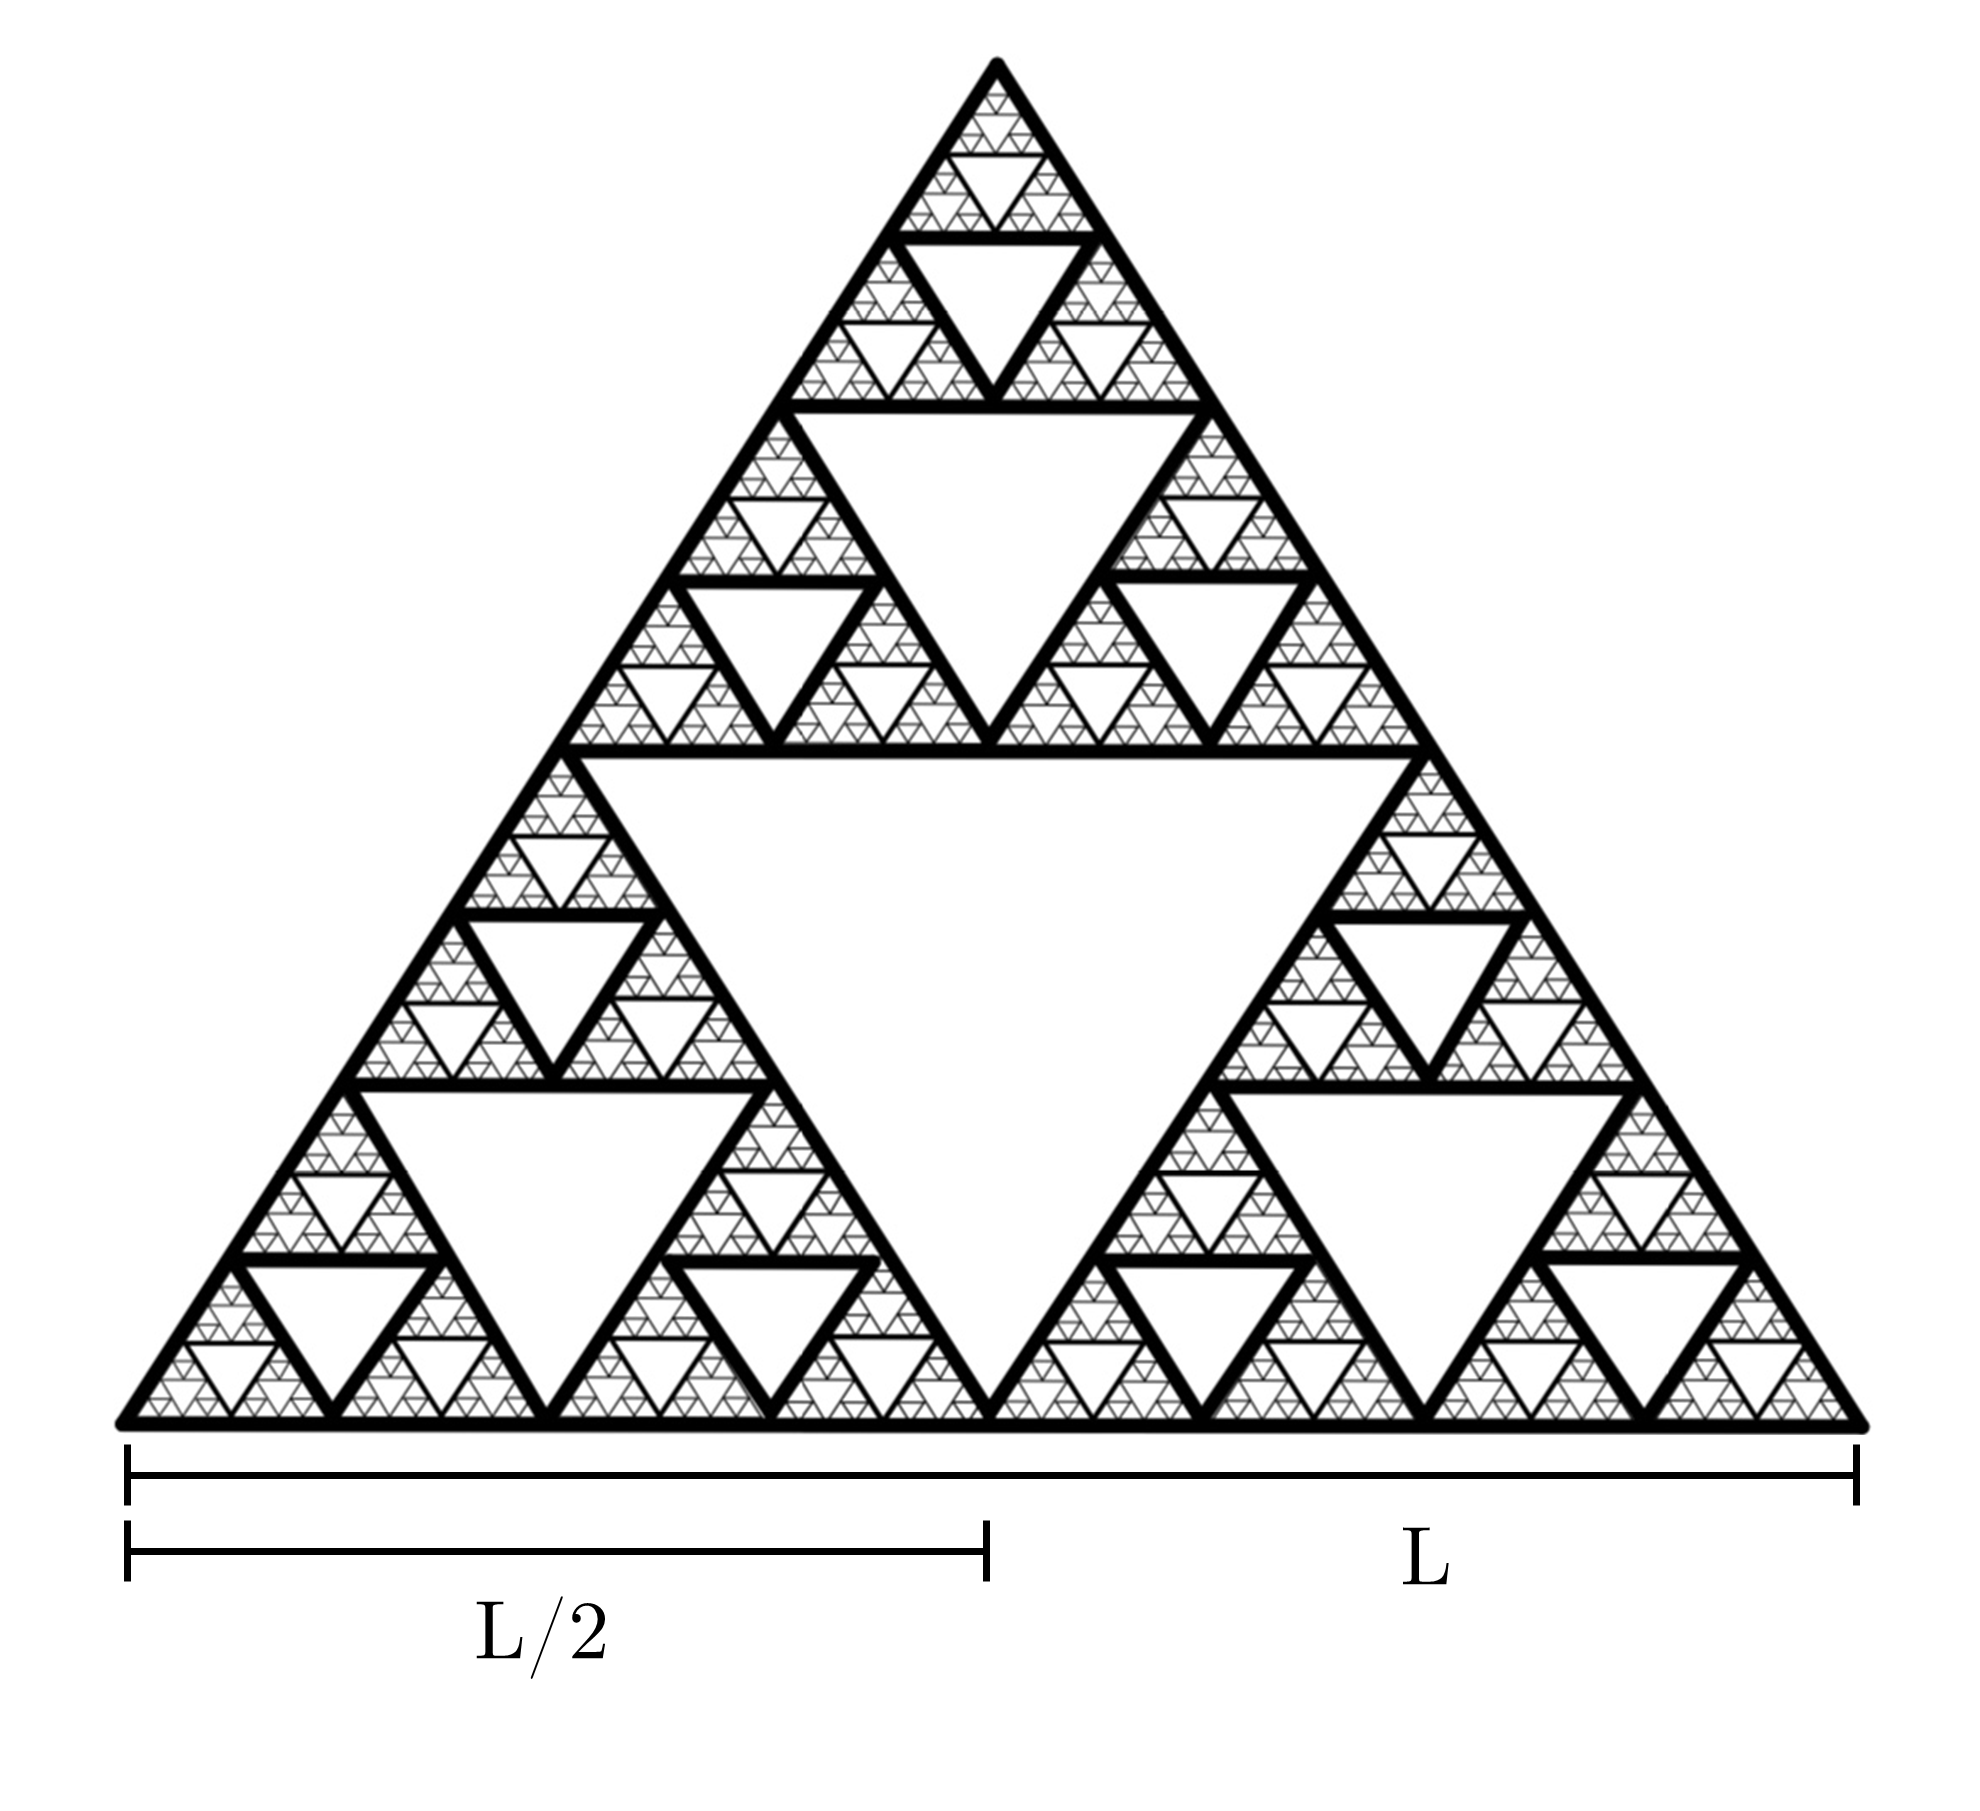
\includegraphics[width=0.5\textwidth]{Images/Sierpinski Triangle.png}
    \caption{Ilustrasi fraktal beraturan bernama segitiga Sierpinski dengan panjang rusuk \(L\) dan ditandai pada bagian \(L/2\).}
\end{figure}
\noindent Jika proses pembagian rusuk menjadi 2 seperti pada 3 bangun sebelumnya dilakukan, maka akan terjadi hal yang berbeda. Bukannya volume tebagi menjadi 2 seperti pada bangun \(1D\) ataupun menjadi 4 seperti pada bangun \(2D\), volume bangun ini terbagi menjadi 3 saat rusuknya dibagi 2. Jika pernyataan tersebut ditulis secara matematis, dimensi dari segitiga Sierpinski ini dapat diketahui.
\begin{align}
    dD \Rightarrow \frac{1}{2} = \left(\frac{1}{3}\right)^\frac{1}{d}
\end{align}
Jika nilai \(d\) dihitung secara numerik, akan diketahui bahwa \(d \approx 1.58\). Atau dapat dikatakan bahwa dimensi fraktal dari segitika Sierpinski memiliki nilai sekitar 1.58. \cite{Mandelbrot1982Fractal}
\par Setelah metode penentuan dimensi fraktal dijelaskan, penjelasan mengenai jenis fraktal yang relevan dengan tulisan ini dapat dilakukan. Dimulai dari gerakan Brownian, yang mana jika dalam 1 dimensi dikenal juga sebagai jalan pemabuk \cite{Schwarz2023Statistics}. Gerakan Brownian memiliki dua pengertian, pertama digunakan untuk mendeskripsikan sebuah gerakan acak yang terjadi pada partikel yang umumnya berada dalam sebuah likuida. Sedangkan yang kedua merujuk pada model matematis yang digunakan untuk merepresentasikan fenomena tersebut. Gerakan Brownian sebagai model matematis dapat direpresentasikan oleh gerakan acak Weiner \(w(t)\) yang bisa diperkenalkan melalui persamaan berikut:
\begin{align}
    w(t,w_0;\xi) = w_0 + \int_{t_0}^t d\tau\xi(\tau), \qquad w(t = t_0) = w_0
\end{align}
Di mana \(w(t,w_0;\xi)\) merepresentasikan posisi partikel pada waktu \(t\) yang bergantung pada posisi awal \(w_0\) dan \(\xi\) yang merupakan "\textit{white noise}" dengan sifat statistik yang didefinisikan oleh,
\begin{align}
    \langle\xi(t_1)...\xi(t_{2n})\rangle_\xi &= \sigma^n \sum_{i_1, ..., i_{2n}\in(1, ..., 2n)} \delta(t_{i_1} - t_{i_2})...\delta(t_{i_{2n-1}} - t_{i_{2n}}) \label{eq:NoiseStat1} \\
    \langle\xi(t_1)...\xi(t_{2n+1})\rangle_\xi &= 0 \label{eq:NoiseStat2}
\end{align}
Di sini penjumlahan dilakukan atas semua kombinasi pasangan yang memungkinkan, \(\langle...\rangle_\xi\) merupakan penulisan untuk rata-rata dari "\textit{white noise}" yang terealisasi, dan \(\sigma\) adalah koefisien difusi. Sebagai contoh, misal \(n=3\) maka bentuk eksplisit dari \ref{eq:NoiseStat1} akan menjadi sebagai berikut:
\begin{align}
    \langle \xi(t_1) ... \xi(t_6) \rangle_\xi = \sigma^3 \Big( & \delta(t_1 - t_2) \delta(t_3 - t_4) \delta(t_5 - t_6) + \delta(t_1 - t_2) \delta(t_3 - t_5) \delta(t_4 - t_6) \nonumber \\
    & + \delta(t_1 - t_2) \delta(t_3 - t_6) \delta(t_4 - t_5) + \delta(t_1 - t_3) \delta(t_2 - t_4) \delta(t_5 - t_6) \nonumber \\
    & + \delta(t_1 - t_3) \delta(t_2 - t_5) \delta(t_4 - t_6) + \delta(t_1 - t_3) \delta(t_2 - t_6) \delta(t_4 - t_5) \nonumber \\
    & + \delta(t_1 - t_4) \delta(t_2 - t_3) \delta(t_5 - t_6) + \delta(t_1 - t_4) \delta(t_2 - t_5) \delta(t_3 - t_6) \nonumber \\
    & + \delta(t_1 - t_4) \delta(t_2 - t_6) \delta(t_3 - t_5) + \delta(t_1 - t_5) \delta(t_2 - t_3) \delta(t_4 - t_6) \nonumber \\
    & + \delta(t_1 - t_5) \delta(t_2 - t_4) \delta(t_3 - t_6) + \delta(t_1 - t_5) \delta(t_2 - t_6) \delta(t_3 - t_4) \nonumber \\
    & + \delta(t_1 - t_6) \delta(t_2 - t_3) \delta(t_4 - t_5) + \delta(t_1 - t_6) \delta(t_2 - t_4) \delta(t_3 - t_5) \nonumber \\
    & + \delta(t_1 - t_6) \delta(t_2 - t_5) \delta(t_3 - t_4) \Big)
\end{align}
Berangkat dari pendefinisian tersebut, fungsi rapat probabilitas \(p(wt|w_0t_0)\) dari proses stokastik \(w(t)\) dapat ditentukan.
\begin{align}
    p(wt|w_0t_0) = \langle\delta(w - w(t,w_0;\xi))\rangle_\xi
\end{align}
Jika fungsi \(\delta\) dibuat sebagai sebuah integral Fourier
\begin{align}
    \delta(x) = \frac{1}{2\pi}\int_{-\infty}^{+\infty} dqe^{iqx}
\end{align}
Maka bentuk berikut ini bisa didapatkan,
\begin{align}
    \langle \delta(w - w(t,w_0;\xi)) \rangle_\xi = \frac{1}{2\pi} \int_{-\infty}^{+\infty} dq \exp{iqw} \langle \exp{-iqw(t,w_0;\xi)} \rangle_\xi
\end{align}
Dengan
\begin{align}
    \langle \exp{-iqw(t,w_0;\xi)} \rangle_\xi = \exp{-iqw_0}\left\langle \exp{-iq\int_{t_0}^t d\tau \xi(\tau)} \right\rangle_\xi \label{eq:<iqw>_xi}
\end{align}
Nilai harap pada bagian kanan persamaan (\ref{eq:<iqw>_xi}) diselesaikan dengan fungsi pembangkit momen yang dituliskan sebagai berikut:
\begin{align}
    \langle e^{Sx} \rangle = M_x (S) = \exp{\kappa S + \frac{1}{2}\sigma_x^2 S^2} 
\end{align}
Jika digunakan \(S=-iq\) dan \(\kappa=0\), maka diperlukan variansi untuk integral pada persamaan (\ref{eq:<iqw>_xi}). Misal integral tersebut dinotasikan sebagai \(I\), maka variansi dapat ditulis sebagai berikut:
\begin{align}
    Var(I) = \left\langle \left(\int_{t_0}^t d\tau \xi(\tau) \right)^2 \right\rangle_\xi - \left\langle \int_{t_0}^t d\tau \xi(\tau) \right\rangle_\xi^2
\end{align}
Dengan menggunakan sifat statistik "\textit{white noise}" pada persamaan (\ref{eq:NoiseStat1}) dan (\ref{eq:NoiseStat2}), didapatkan hasil sebagai berikut:
\begin{align}
    Var(I) = \sigma^2 (t-t_0)
\end{align}
Dengan begitu didapatkan,
\begin{align}
    \left\langle \exp{-iq\int_{t_0}^t d\tau \xi(\tau)} \right\rangle_\xi = \exp{-\frac{1}{2}q^2\sigma^2(t-t_0)} \label{eq:<iqint>_xi}
\end{align}
Persamaan (\ref{eq:<iqint>_xi}) tersebut disubstitusi ke persamaan (\ref{eq:<iqw>_xi}) untuk mendapatkan bentuk berikut:
\begin{align}
    p(wt|w_0t_0) = \frac{1}{2\pi}\int_{-\infty}^{+\infty} dqe^{iq(w-w_0)}\exp{-\frac{1}{2}\sigma q^2(t-t_0)}
\end{align}
Yang jika persamaan tersebut diselesaikan, akan didapat bentuk akhir dari fungsi rapat probabilitas untuk gerakan Brownian. \cite{Huang1978Stochastic}
\begin{align}
    p(wt|w_0t_0) = \frac{1}{\sqrt{2\pi\sigma(t-t_0)}}\exp{-\frac{(w-w_0)^2}{2\sigma(t-t_0)}}, \qquad t>t_0 \label{eq:pdfBrownian}
\end{align}
Di mana persamaan (\ref{eq:pdfBrownian}) terebut menunjukan relasi
\begin{align}
    (w-w_0) \propto (\sigma(t-t_0))^{\frac{1}{2}} \label{eq:w-w0_relation}
\end{align}
Lalu persamaan (\ref{eq:w-w0_relation}) menunjukan relasi pembagian skala yang dapat menunjukan dimensi fraktal dari gerakan Brownian. Dengan menggunakan metode perubahan skala terhadap perubahan volume tersebut, nilai dari dimensinya bisa didekati dan akan didapatkan nilai 2. Maka dari itu, bisa juga disimpulkan bahwa dimensi fraktal dari gerakan Brownian adalah 2. \cite{Sutton2024Brownian}
\par Bentuk fraktal berikutnya adalah Levy \textit{flight} yang merupakan bentuk generalisasi natural dari gerakan Brownian. Perbedaan mendasar dari kedua bentuk ini adalah pada gerakan Brownian, arah dari setiap langkah itu acak, namun jarak tiap langkahnya sama. Sedangkan pada penerbangang Levy, baik arah maupun jarak tiap langkah keduanya acak. Sehingga pada Levy \textit{flight} terkadang terjadi lompatan jarak jauh secara tiba-tiba \cite{Viswanathan2008Levy}. Proses acak dari Levy ini dapat didefinisikan oleh persamaan diferensial stokastik
\begin{align}
    \dot{x}(t) = \xi_L(t), \qquad x(t_0) = x_0
\end{align}
Dengan "\textit{white noise}" Levy yang memiliki karakteristik fungsional mengikuti
\begin{align}
    \left\langle\exp{i\int_{t_0}^t d\tau q(\tau)\xi_L(\tau)}\right\rangle_{\xi_L} = \exp{-\sigma_\alpha \int_{t_0}^t d\tau |q(\tau)|^\alpha}
\end{align}
Di mana \(\sigma_\alpha\) merupakan intensitas \textit{noise} Levy, \(\alpha\) adalah indeks Levy, dan \(\langle ...\rangle_{\xi_L}\) adalah rata-rata dari setiap realisasi yang memungkinkan untuk \textit{noise} Levy. Lalu, karena pada dasarnya Levy \textit{flight} adalah bentuk lebih umum dari gerakan Brownian, maka metode untuk mendapatkan fungsi rapat probabilitasnya akan serupa. Di mana pada Levy \textit{flight} akan didapai fungsi berbentuk
\begin{align}
    p_L(xt|x_0t_0) = \frac{1}{2\pi}\int_{-\infty}^{\infty}dqe^{iq(x-x_0)}\exp{-\sigma_\alpha |q|^\alpha (t-t_0)}, \qquad t>t_0
\end{align}
Yang mengarahkan kepada hubungan yang dapat digunakan untuk menentukan dimensi fraktal dari Levy \textit{flight}. Hubungan tersebut adalah,
\begin{align}
    (x-x_0) \propto (\sigma_\alpha (t-t_0))^\frac{1}{\alpha}, \qquad 1<\alpha\leq 2
\end{align}
Berdasarkan definisi dari dimensi fraktal, dapat dikatakan fraktal dari Levy \textit{flight} adalah \(\alpha\) yang memiliki nilai \(1<\alpha\leq 2\). Jika nilai dari \(\alpha\) sama degan 2, maka Levy \textit{flight} berubah menjadi gerakan Brownian. \cite{Laskin2018Fractional}

\section{Mekanika Kuantum}
Mekanika kuantum dibangun oleh 6 postulat. Postulat pertama adalah keadaan dari sebuah sistem kuantum dinyatakan secara lengkap oleh fungsi gelombang \(\Psi(x,t)\) yang bergantung pada posisi dari partikel serta waktu. Fungsi ini dikenal sebagai fungsi gelombang atau fungsi keadaan yang memiliki sifat \(\Psi^*(x,t)\Psi(x,t)dx\) merupakan probabilitas untuk menemukan partikel pada \(dx\) di waktu \(t\). Hal ini disebut dengan interpretasi probabilistik Born yang mana harus mengikuti kondisi normalisasi berikut:
\begin{align}
    \int_{-\infty}^{+\infty}|\Psi(x,t)|^2 dx = 1 \label{eq:TotalProbability}
\end{align}
Sifat lain dari fungsi gelombang adalah fungsi tersebut haruslah memiliki nilai tunggal, kontinu, dan terbatas \cite{Peres2004Quantum}.
% Secara umum, fungsi memiliki sifat yang analog dengan vektor sehingga terkadang fungsi gelombang dinyatakan sebagai vektor keadaan \(|\psi\rangle\) \cite{Griffiths_Schroeter_2018}. Notasi \(|\psi\rangle\) disebut dengan ket dan dualnya \(\langle \psi|\) disebut dengan bra yang merupakan notasi Dirac. Dalam sumber lain, postulat 1 ini dinyatakan dalam bunyi; keadaan dari sebuah sistem kuantum didefinisikan oleh sebuah vektor keadaan \(|\psi\rangle\) yang berada pada sebuah ruang kompleks Hilbert. Prinsip superposisi berlaku pada ruang ini, yang mana jika \(|\phi_1\rangle, |\phi_2\rangle, ..., |\phi_n\rangle\) adalah ket pada ruang Hilbert, maka kombinasi linear
% \begin{align}
%     |\chi\rangle = \sum_{i=1}^n a_i |\phi_i\rangle
% \end{align}
% juga merupakan sebuah keadadan valid yang berada pada ruang Hilbert. Vektor keadaan ini mengikuti normalisasi berikut:
% \begin{align}
%     \langle\psi|\psi\rangle = 1
% \end{align}
% Jika sebuah keadaan membentuk superposisi dengan keadaan lain, normalisasi mengimplikasikan bahwa total penjumlaham kuadrat dari koefisien-koifisiennya haruslah sama dengan 1 \cite{McMahon2013Quantum}.
% \begin{align}
%     \langle\chi|\chi\rangle = \sum_{i=1}^n |a_i|^2 = 1
% \end{align}
Postulat kedua adalah untuk setiap besaran teramati (\textit{obsevable}) dalam mekanika klasik terdapat operator linear Hermitian-nya dalam mekanika kuantum. Postulat ketiga adalah dalam pengukuran \textit{obsevable} apapun yang terasosiasi dengan operator \(\hat{A}\), nilai yang bisa diamati hanyalah nilai eigen dari operator tersebut yang memenuhi persamaan,
\begin{align}
    \hat{A}\Psi = a\Psi
\end{align}
Jika sistem berada dalam keadaan eigen dari operator \(\hat{A}\) dengan nilai eigen \(a\), maka pengukuran dari besaran \(A\) akan selalu menghasilkan nilai \(a\). Meski demikian, keadaan awalnya tidak harus merupakan keadaan eigen dari \(\hat{A}\). Keadaan ini dapat dinyatakan sebagai kombinasi linear dari himpunan lengkap vektor eigen dari \(\hat{A}\), yaitu
\begin{align}
    \Psi = \sum_i^n a_i \Psi_i
\end{align}
di mana jumlah \(n\) tersebut dimungkinkan menuju tak terhingga. Dalam hal ini, pengukuran dari \(A\) akan menghasilkan salah satu nilai eigen \(a_i\), tetapi nilai eigen mana yang akan dihasilkan tidak diketahui. Postulat keempat adalah jika sebuah sistem dinyatakan dengan fungsi gelombang ternormalisasi, maka nilai harap dari \textit{obsevable} yang terasosiasi dengan \(\hat{A}\) diberikan oleh
\begin{align}
    \langle \hat{A} \rangle = \int_{-\infty}^{+\infty}\Psi^* \hat{A} \Psi dx
\end{align}
Postulat kelima adalah keadaan sebuah sistem berevolusi terhadap waktu mengikuti persamaan Schrodinger bergantung waktu. Terakhir postulat keenam adalah fungsi gelombang untuk sistem banyak fermion harus antisimetri terhadap pertukaran dua fermion mana pun. \cite{Zettili2009Quantum}

\subsection{Persamaan Schrodinger}
Persamaan Schrodinger dapat ditinjau setidaknya dengan 3 cara. Persamaan diferensial Schrodinger, representasi matriks Heisenberg, dan \textit{path integral} Feynman \cite{Feynman1948Quantum}. Representasi yang akan ditinjau pada tulisan ini adalah milik Feynman yang mana mempertimbangkan seluruh kemungkinan jalur yang ditempuh sebuah partikel untuk mencapai suatu keadaan tertentu. Ilustrasinya digambarkan sebagai berikut:
\begin{figure} [H]
    \centering
    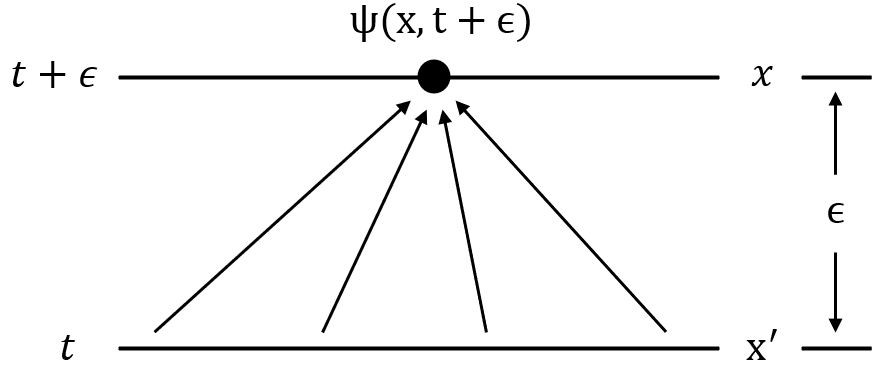
\includegraphics[width=0.5\textwidth]{Images/Feynman Setup.png}
    \caption{\textit{Setup} awal reprsentasi Feynman terhadap persamaan Schrodinger.}
\end{figure}
Ilustrasi tersebut dapat dituangkan secara matematis dalam persamaan berikut:
\begin{align}
    \Psi(x,t+\epsilon) = \int_{-\infty}^{+\infty} G(x,x')\Psi(x',t)dx'
    \label{eq:FeynmanSetup}
\end{align}
Di sini \(\Psi(x',t)\) berevolusi menjadi \(\Psi(x,t+\epsilon)\) melalui sebuah propagator \(G(x,x')\) (dalam beberapa referensi disebut juga sebagai Kernel) dalam rentang waktu \(\epsilon\) di mana semua nilai \(x'\) dapat dipertimbangkan \cite{Das2019Field}. Bentuk propagator pada \ref{eq:FeynmanSetup} belum diketahui. Namun \(G(x,x')\) diasumsikan memiliki bentuk eksponen sebagai berikut:
\begin{align}
    G(x,x') = Ae^{\frac{i\mathcal{S}(x,x')}{\hbar}}
\end{align}
Di mana \(\mathcal{S}\) merupakan aksi yang dilakukan oleh partikel dan dapat didefinisikan sebagai,
\begin{align}
    \mathcal{S} = \int_t^{t+\epsilon}\mathcal{L}dt \label{eq:Action}
\end{align}
Dengan \(\mathcal{L}\) merupakan Lagrangian dari partikel yang ditinjau \cite{Kibble2004Classical}. Di sini diasumsikan solusi dari integral pada aksi memiliki bentuk rata-rata Lagrangian dikali waktu tempuh.
\begin{align}
    \mathcal{S} = \overline{\mathcal{L}}\epsilon
\end{align}
Lagrangian ini dapat dituliskan dalam bentuk
\begin{align}
    \overline{\mathcal{L}} &= \overline{K} - \overline{V} = \frac{m}{2}\left(\frac{\Delta x}{\Delta t}\right)^2 - \overline{V}
\end{align}
Jika dianggap potensial rata-rata sama dengan potensial pada titik di tengah \(x\) dan \(x'\), maka akan akan didapat bentuk
\begin{align}
    \overline{\mathcal{L}} = \frac{m}{2}\frac{(x-x')^2}{\epsilon^2} - V\left(\frac{x+x'}{2}\right)
\end{align}
Yang kemudian disubstitusi kembali ke \(G(x,x')\) untuk mendapatkan bentuk lebih lengkap dari fungsi \(\Psi(x,t+\epsilon)\).
\par Untuk memudahkan dalam perhitungan, diperkenalkan sebuah parameter baru \(\gamma\) di mana \(\gamma = x - x'\) dan \(d\gamma = -dx'\). Sehingga, fungsi \(\Psi(x,t+\epsilon)\) menjadi
\begin{align}
    \Psi(x,t+\epsilon) = \int_{-\infty}^{+\infty} A \exp{\frac{im}{2\hbar\epsilon}\gamma^2} \exp{\frac{i\epsilon}{\hbar}V\left(x-\frac{\gamma}{2}\right)}\Psi(x-\gamma,t)d\gamma
\end{align}
Bentuk eksponen kedua dapat disederhanakan dengan ekspansi deret Taylor dan diambil 2 suku awalnya saja.
\begin{align}
    \Psi(x,t+\epsilon) = \int_{-\infty}^{+\infty} A \exp{\frac{im}{2\hbar\epsilon}\gamma^2} \left(1 - \frac{i\epsilon}{\hbar}V\left(x - \frac{\gamma}{2}\right)\right)\Psi(x-\gamma,t)d\gamma
    \label{eq:VTaylor1}
\end{align}
Bagian \(\Psi(x-\gamma,t)\) juga dapat diekspansi menggunakan deret Taylor dan diambil 3 suku pertamanya.
\begin{align}
    \Psi(x-\gamma,t) = \Psi(x,t) - \frac{\partial}{\partial x}\Psi(x,t)\gamma + \frac{1}{2}\frac{\partial^2\Psi(x,t)}{\partial x^2} \gamma^2
    \label{eq:Psi(xgt)Taylor}
\end{align}
Dari ekspansi pada persamaan (\ref{eq:Psi(xgt)Taylor}) tersebut dapat dilakukan perhitungan orde ke-0 untuk memperoleh nilai \(A\).

\begin{align}
    % \int_{-\infty}^{+\infty}\exp{\frac{im}{2\hbar\epsilon}\gamma^2}d\gamma &= \sqrt{-\frac{2\hbar\pi\epsilon}{im}} = \frac{1}{A} \\
    A &= \sqrt{\frac{-im}{2\hbar\pi\epsilon}} \label{eq:FeynmanA}
\end{align}
Persamaan (\ref{eq:FeynmanA}) dapat disubstitusi kembali ke fungsi \(\Psi(x,t+\epsilon)\). Atau untuk menyederhanakan penulisan, digunakan tetap dalam bentuk \(A\)-nya karena bentuk eksplisitnya sudah diketahui.
\par Sejauh ini bentuk persamaan dari \ref{eq:VTaylor1} belum berubah dan bisa saja diselesaikan integralnya dalam bentuk itu. Namun, untuk menyederhanakan perhitungan, bentuk potensialnya diekspansi lagi menggunakan deret Taylor dan mengambil suku pertamanya saja. Hal ini bisa dilakukan karena pada suku ke-2 dan seterusnya akan ada \(\gamma\) yang akan bertemu dengan \(\epsilon\). Kedua variabel tersebut sangat kecil nilainya sehingga jika dikalikan satu sama lain akan didapat hasil yang sangat-sangat kecil sehingga bisa diabaikan. Dengan begitu akan didapat bentuk persamaan sebagai berikut:
\begin{align}
    \Psi(x,t+\epsilon) = A\int_{-\infty}^{+\infty}\exp{\frac{im}{2\hbar\epsilon}\gamma^2} \left(1-\frac{i\epsilon}{\hbar}V(x)\right)\Psi(x-\gamma,t)d\gamma
\end{align}
Jika menggunakan ekspansi Taylor \(\Psi(x-\gamma,t)\) pada persamaan \ref{eq:Psi(xgt)Taylor}, maka integral dari permasalahan ini dapat dieselesaikan menggunakan 3 integral \(I_1 + I_2 + I_3\) yang dapat dikerjakan secara terpisah. Hasil dari integral-integral tersebut adalah sebagai berikut:
\begin{align}
    I_1 &= \left(1 - \frac{i\epsilon}{\hbar}V(x)\right)\Psi(x,t) A\int_{-\infty}^{+\infty} \exp{\frac{im}{2\hbar\epsilon}\gamma} d\gamma =\left(1 - \frac{i\epsilon}{\hbar}V(x)\right)\Psi(x,t) \\
    I_2 &= -\frac{\partial\Psi(x,t)}{\partial(x)} A\int_{-\infty}^{+\infty} \exp{\frac{im}{2\hbar\epsilon}\gamma}\gamma d\gamma = 0 \\
    I_3 &= \frac{1}{2}\frac{\partial^2\Psi(x,t)}{\partial x^2} A\int_{-\infty}^{+\infty} \exp{\frac{im}{2\hbar\epsilon}\gamma^2}d\gamma = \frac{i\hbar\epsilon}{2m} \frac{\partial^2\Psi(x,t)}{\partial x^2} 
\end{align}

Jika semua hasil tersebut digabung, akan didapatkan bentuk,
\begin{align}
    \Psi(x,t+\epsilon) = \left(1-\frac{i\epsilon}{\hbar}V(x)\right)\Psi(x,t) + \frac{i\hbar\epsilon}{2m}\frac{\partial^2\Psi(x,t)}{\partial x^2}
\end{align}
Persamaan tersebut dapat disusun ulang menjadi
\begin{align}
    \frac{\Psi(x,t+\epsilon)-\Psi(x,t)}{\epsilon} = \frac{i\hbar}{2m} \frac{\partial^2\Psi(x,t)}{\partial x^2} - \frac{i}{\hbar}V(x)\Psi(x,t)
    \label{eq:ddtPsiDefinition}
\end{align}
Di sini diketahui nilai \(\epsilon\) sangatlah kecil sehingga dapat dikatakan bahwa bentuk bagian kiri dari persamaan \ref{eq:ddtPsiDefinition} merupakan definisi dari turunan pertama terhadap waktu. 
\begin{align}
    \frac{\partial\Psi(x,t)}{\partial t} = \frac{i\hbar}{2m}\frac{\partial^2\Psi(x,t)}{\partial x^2} - \frac{i}{\hbar}V(x)\Psi(x,t)
\end{align}
Di sini, kedua ruas dapat dikali dengan \(i\hbar\) untuk mendapatkan
\begin{align}
    i\hbar\frac{\partial\Psi(x,t)}{\partial t} = -\frac{\hbar^2}{2m} \frac{\partial^2\Psi(x,t)}{\partial x^2} + V(x)\Psi(x,t)
    \label{eq:Schrodinger}
\end{align}
Yang mana merupakan bentuk persamaan Schrodinger yang banyak diketahui. \cite{Derbes1996Feynman}
\par Meski tidak disebutkan secara langsung, pendekatan Feynman ini pada dasarnya adalah pendekatan persamaan Schrodinger melalui gerakan Brownian yang yang merupakan sebuah fraktal acak yang mana membuka jalan kepada penerapan fraktal pada mekanika kuantum. Penerapan fraktal ini dilanjutkan oleh Nick Laskin yang melakukan generalisasi persamaan Schrodinger menggunakan Levy \textit{flight} \cite{Herrmann2014Fractional}. Pendekatan ini bisa disebut mekanika kuantum fraksional, atau lebih spesifik, persamaan Schrodinger Fraksional yang diperkenalkan oleh Laskin dengan operator Hamiltonian yang berbentuk:
\begin{align}
    \hat{H_\alpha}(\hat{\textbf{p}}, \hat{\textbf{r}}) = D_\alpha|\hat{\textbf{p}}|^\alpha + V(\hat{\textbf{r}}), \qquad 1<\alpha\leq 2 \label{eq:FractionalHamiltonian}
\end{align}
Di mana \(D_\alpha\) merupakan koefisien fraksional yang pada tulisan ini didefinisikan oleh \(D_\alpha = (1/2m)^{\alpha/2}\) dan \(\alpha\) merupakan indeks Levy yang berikutnya akan disebut sebagai parameter fraksional \cite{Xia2024Performance}. Untuk mendapatkan persamaan Schrodinger fraksional, digunakan permulaan yang sama seperti persamaan (\ref{eq:FeynmanSetup}) dengan notasi yang sedikit diubah menjadi.
\begin{align}
    \Psi(x,t+\epsilon) = \int_{-\infty}^{+\infty}dx' K_L(x,t+\epsilon |x',t) \Psi(x',t)
\end{align}
Dengan \(K_L(x,t+\epsilon |x',t)\) merupakan kernel. Untuk partikel bebas, representasi momentum dari kernel ini dapat dituliskan sebagai berikut:
\begin{align}
    K_L^{(0)}(x,t+\epsilon |x',t) = \frac{1}{2\pi\hbar} \int_{-\infty}^{+\infty}dp \exp{\frac{i}{\hbar}(p(x-x') - D_\alpha |p|^\alpha (t+\epsilon - t))} \label{eq:FreePartKernel}
\end{align}
Dengan menggunkan aproksimasi \(\int_t^{t+\epsilon} d\tau V(x) \approx \epsilon V((x+x')/2) \) dan persamaan (\ref{eq:FreePartKernel}), bisa didapatkan bentuk berikut:
\begin{align}
    \Psi(x,t+\epsilon) =& \int_{-\infty}^{+\infty}dx' \frac{1}{2\pi\hbar} \int_{-\infty}^{+\infty} dp \exp \biggl\{\frac{i}{\hbar}\biggl(p(x-x') \notag \\
    &- D_\alpha |p|^\alpha \epsilon - \epsilon V\left(\frac{x+x'}{2}\right)\biggl)\biggl\} \Psi(x',t) \label{eq:FractionalPathInt1}
\end{align}
Bagian kiri dan kanan persamaan (\ref{eq:FractionalPathInt1}) dapat diekspansi menggunakan deret Taylor untuk mendapatkan
\begin{align}
    \Psi(x,t) + \epsilon\frac{\partial\Psi(x,t)}{\partial(t)} =& \int_{-\infty}^{+\infty}dx' \frac{1}{2\pi\hbar} \int_{-\infty}^{+\infty} dp e^\frac{ip(x-x')}{\hbar} \times \notag\\
    &\left(1 - \frac{iD_\alpha |p|^\alpha \epsilon}{\hbar}\right) \left(1 - \frac{1}{\hbar}\epsilon V\left(\frac{x+x'}{2}\right)\right)\Psi(x',t) \label{eq:FractionalPathInt2}
\end{align}
Untuk menyelesaikan persamaan (\ref{eq:FractionalPathInt1}), Laskin memperkenalkan derivatif kuantum fraksional Riesz 1D yang didefinisikan oleh,
\begin{align}
    (\hbar\nabla)^\alpha \Psi(x,t) = -\frac{1}{2\pi\hbar}\int_{-\infty}^{+\infty}dpe^{i\frac{px}{\hbar}}|p|^\alpha \Phi(p,t) \label{eq:RieszDef}
\end{align}
Dengan \(\Psi(x,t)\) dan \(\Phi(p,t)\) terhubung melalui sebuah transformasi Fourier.
\begin{align}
    \Psi(x,t) &= \frac{1}{2\pi\hbar}\int_{-\infty}^{+\infty}dpe^{i\frac{px}{\hbar}}\Phi(p,t)\\
    \Phi(p,t) &= \int_{-\infty}^{+\infty}dxe^{-i\frac{px}{\hbar}}\Psi(x,t)
\end{align}
Sehingga didapat persamaan berikut,
\begin{align}
    \Psi(x,t) + \epsilon\frac{\partial \Psi(x,t)}{\partial t} = \Psi(x,t) + \frac{i}{\hbar}D_\alpha \epsilon (\hbar\nabla)^\alpha \Psi(x,t) - \frac{i}{\hbar}\epsilon V(x)\Psi(x,t)
\end{align}
Yang mana jika disederhanakan akan didapat bentuk dari persamaan Schrodinger fraksional 1 dimensi. 
\begin{align}
    i\hbar \frac{\partial\Psi(x,t)}{\partial t} = -D_\alpha(\hbar\nabla)^\alpha \Psi(x,t) + V(x)\Psi(x,t), \qquad 1<\alpha\leq 2 \label{eq:Fractional1DSchrodinger}
\end{align}
Jika nilai dari parameter fraksional \(\alpha\) pada persamaan \ref{eq:Fractional1DSchrodinger} ditetapkan menjadi 2, maka persamaan akan kembali menjadi persamaan Schrodinger biasa seperti pada persamaan \ref{eq:Schrodinger}. \cite{Laskin2018Fractional}

\subsection{Kasus Khusus: Sumur Potensial tak Hingga}
Permasalahan yang paling mendasar yang dipelajari pada fisika kuantum adalah permasalah sumur potensial tak hingga 1 dimensi. Permasalahan ini relevan dengan tulisan ini karena permasalahan mesin panas yang akan diuraikan dikembangkan dari permasalahan ini. Diberikan sebuah partikel 1 dimensi bermassa \(m\) yang terjebak di antara 2 potensial bernilai tak hingga. Sedangkan partikel itu sendiri berada pada potensial bernilai 0 yang memiliki lebar \(L\) pada sumbu \(x\). Permasalahan tersebut diilustrasikan sebagai berikut,
\begin{figure}[H]
    \centering
    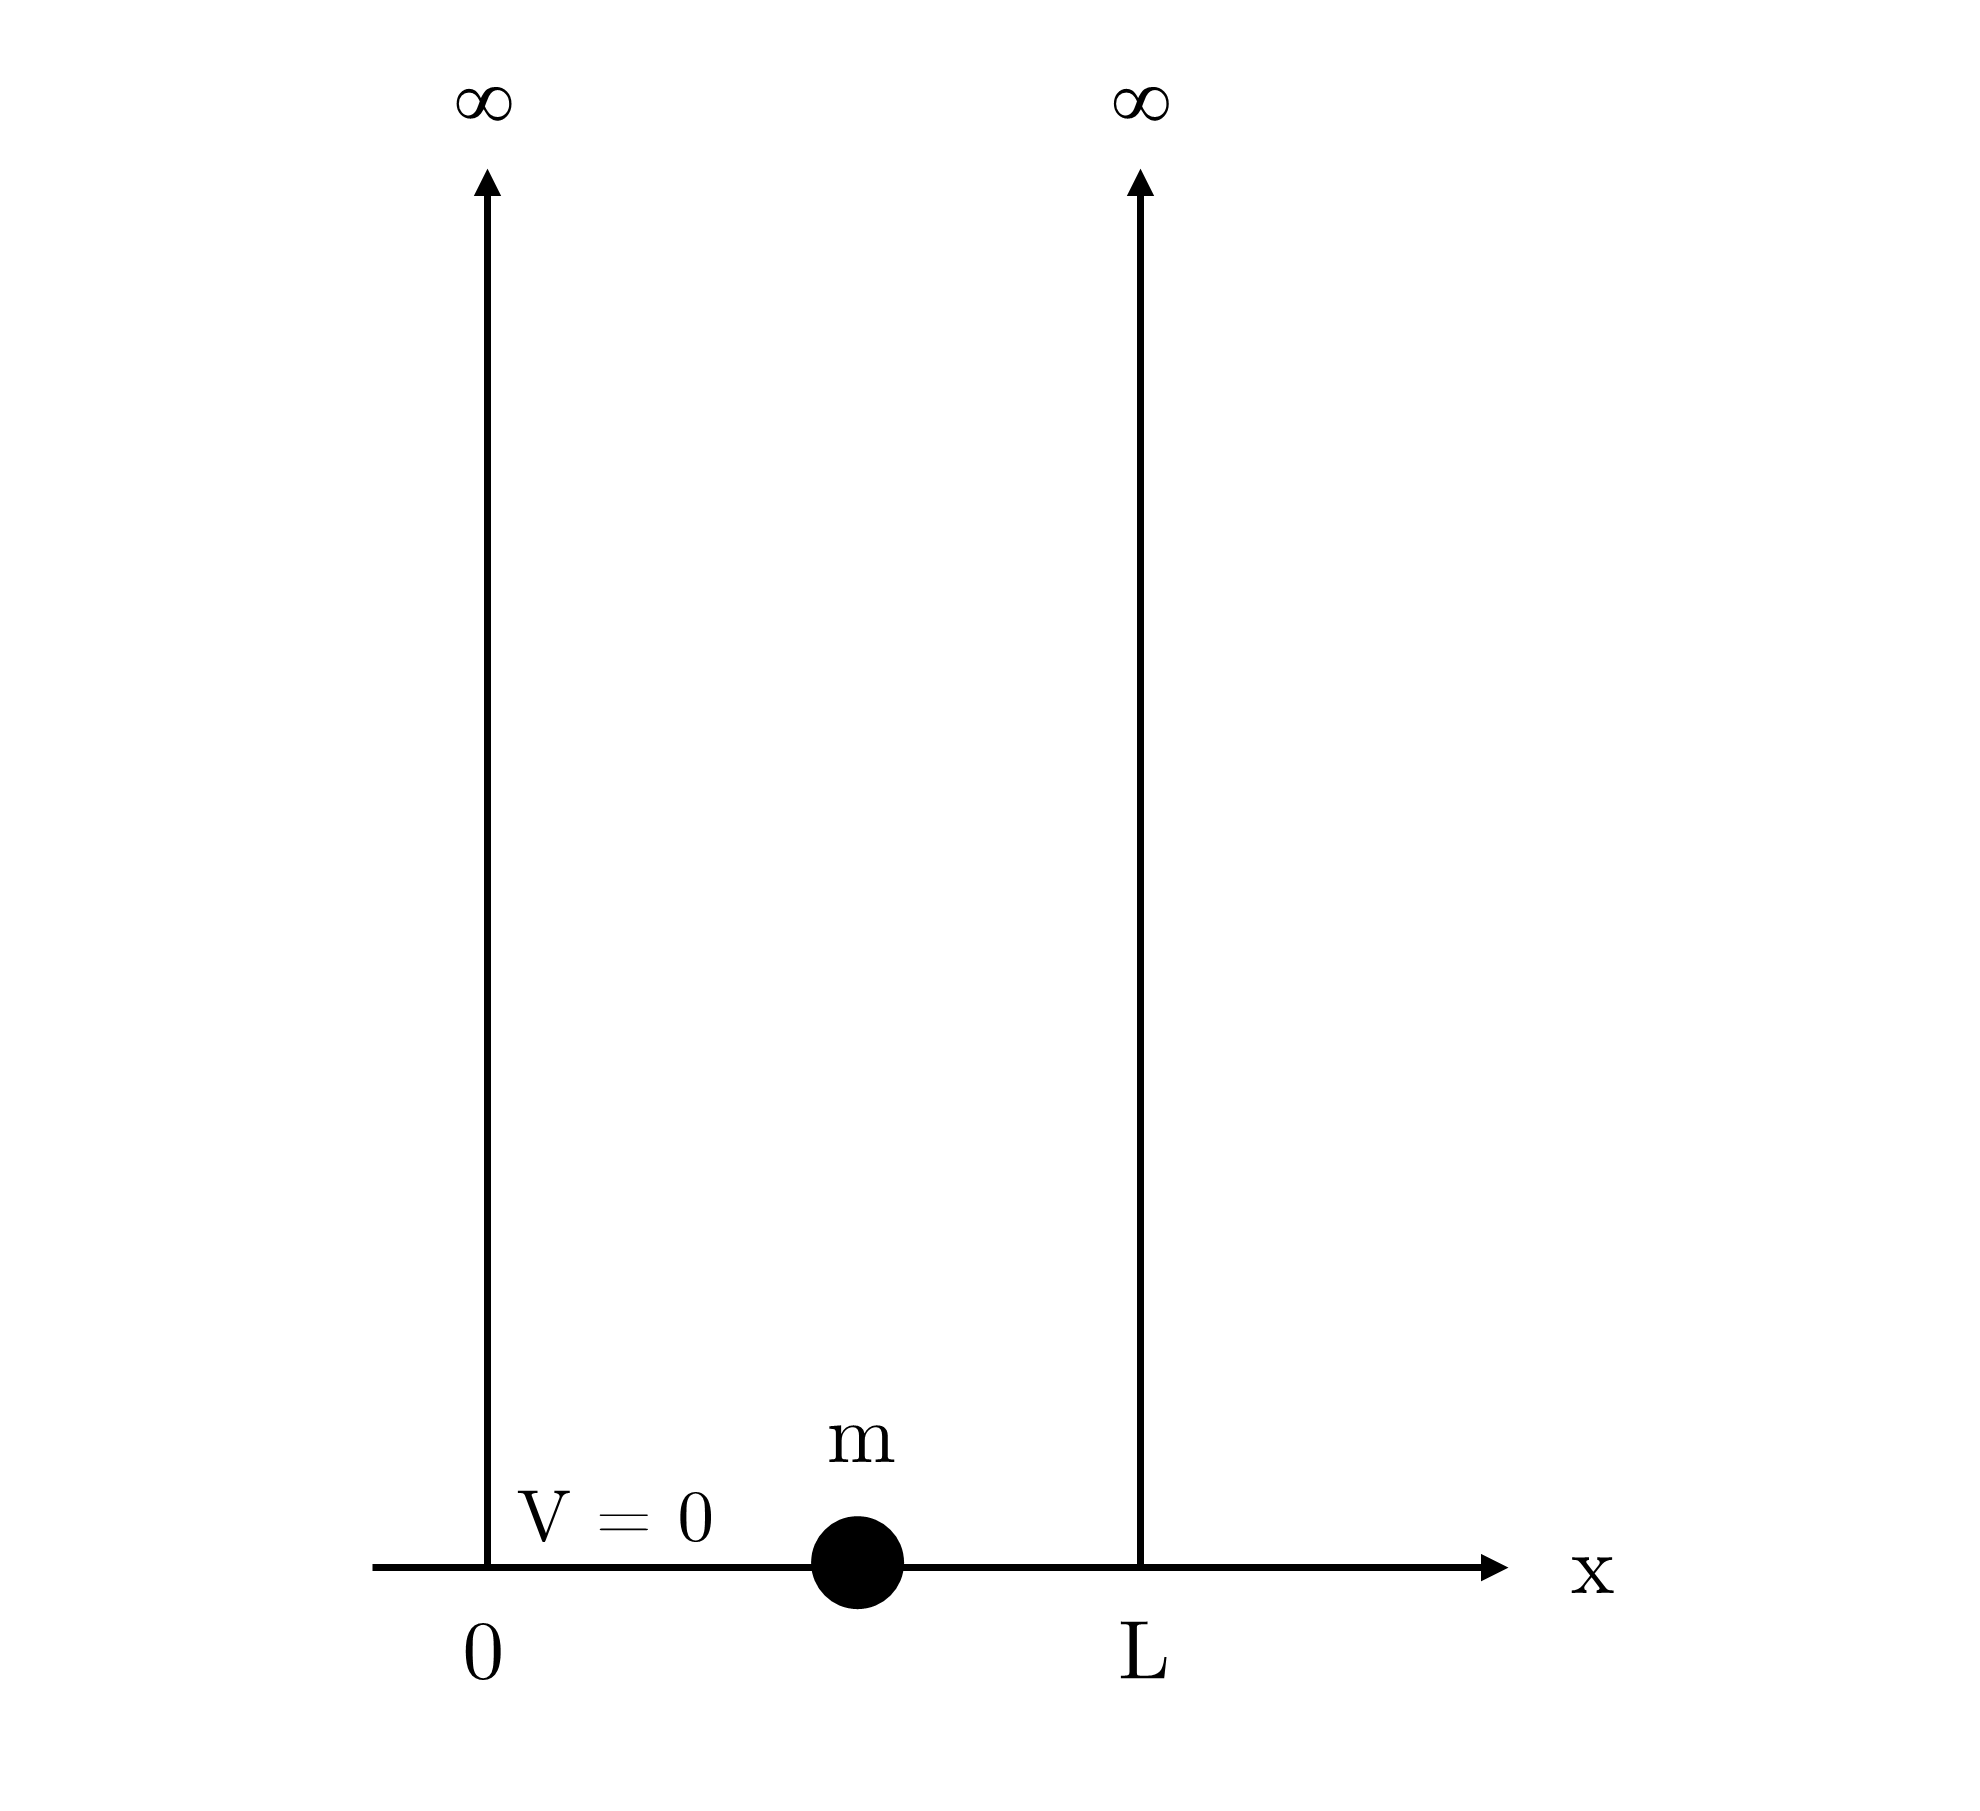
\includegraphics[width=0.5\textwidth]{Images/1D IPW.png}
    \caption{Partikel Bermassa \(m\) dalam Sumur Potensial tak Hingga 1 Dimensi}
    \label{fig:1DIPW}
\end{figure}
\noindent Potensial tak hingga yang menjebak partikel dimaksudkan agar partikel dapat dipastikan berada di dalam sumur \cite{Sathish2014Particle}. Dengan begitu, normalisasi pada persamaan (\ref{eq:TotalProbability}) berubah menjadi
\begin{align}
    \int_0^L |\psi(x)|^2 dx = 1 \label{eq:NormalizationIPW}
\end{align}
Lalu potensial yang digunakan dapat ditulis sebagai berikut:
\begin{align}
    V(x) =
    \begin{cases}
        0 & 0 < x < L \\
        \infty & \text{lainnya} 
    \end{cases} \label{eq:IPWCondition}
\end{align}
Permasalahan ini dapat diselesaikan dengan separasi variabel dari persamaan Schrodinger.
\begin{align}
    \Psi(x,t) = \psi(x)\phi(t)
\end{align}
Untuk mendapatkan komponen bergantung dan tak-bergantung waktu.
\begin{align}
    \frac{d\phi(t)}{dt} &= -\frac{iE}{\hbar}\phi(t) \label{eq:PhiNonFrac1} \\
    E\psi(x) &= -\frac{\hbar^2}{2m} \frac{d^2\psi(x)}{dx^2} + V(x)\psi(x) \label{eq:PsiNonFrac}
\end{align}
Dengan \(E\) merupakan konstanta separasi dan juga energi dari partikel \cite{Griffiths_Schroeter_2018}. Pada rentang \(0<x<L\) potensial 0, sehingga persamaan Schrodinger tak bergantung waktu (\ref{eq:PsiNonFrac}) dapat ditulis menjadi;
\begin{align}
    \frac{d^2\psi}{dx^2} + \frac{2mE}{\hbar^2}\psi = 0 \label{eq:TimeIndpSchrodinger}
\end{align}
Persamaan tersebut memiliki pola persamaan diferensial orde 2 yang cukup umum yaitu persamaan osilator harmonik. Untuk itu, ditentukan sebuah konstanta berikut:
\begin{align}
    k^2 = \frac{2mE}{\hbar^2}
\end{align}
Dengan demikian, persamaan (\ref{eq:TimeIndpSchrodinger}) berubah menjadi
\begin{align}
    \frac{d^2\psi}{dx^2} + k^2\psi = 0 \label{eq:StandingWaveEquation}
\end{align}
Solusi umum dari persamaan (\ref{eq:StandingWaveEquation}) adalah
\begin{align}
    \psi(x) = A\cos{kx} + B\sin{kx} \label{eq:GenSolution}
\end{align}
Pada persmasalahan ini, dapat dirumuskan syarat batas berikut:
\begin{align}
    \psi(x=0) &= 0 \label{eq:Boundary1} \\
    \psi(x=L) &= 0 \label{eq:Boundary2}
\end{align}
Dari syarat batas pertama (\ref{eq:Boundary1}) didapat \(A=0\) dan dari syarat batas kedua (\ref{eq:Boundary2}) didapat \(\sin{kx}=0\). Nilai \(\sin\) menjadi 0 pada kelipatan bilangan bulat dari \(\pi\). Sehingga didapatkan nilai \(k = n\pi/L\). Nilai dari \(E\) atau energi partikel dapat ditentukan dengan menggunakan kedua nilai \(k\) dan ditulis sebagai,
\begin{align}
    E_n = \frac{\hbar^2\pi^2}{2mL^2}n^2 \label{eq:EigenEnergy}
\end{align}
Dengan \(n\) merupakan bilangan bulat positif. Lalu dari normalisasi pada persamaan (\ref{eq:NormalizationIPW}), solusi eksplisit dari fungsi gelombang tak bergantung waktu pada potensial tak hingga dapat dituliskan sebagai berikut:
\begin{align}
    \psi(x) = \sqrt{\frac{2}{L}} \sin{\left\{\frac{n\pi}{L}x\right\}} \label{eq:PsiXSolution}
\end{align}
% Kemudian dapat ditinjau komponen bergantung waktu pada persamaan (\ref{eq:PhiNonFrac1}) yang mana memiliki solusi
% \begin{align}
%     \phi(t) = \cos{\left\{-\frac{E}{\hbar}t \right\}} + i\sin{\left\{-\frac{E}{\hbar}t\right\}}
% \end{align}
% Dengan mempertimbangkan bentuk kuantisasi energi pada persamaan (\ref{eq:EigenEnergy}), bentuk eksplisit dari fungsi gelombang bergantung waktu dapat ditulis sebagai berikut:
% \begin{align}
%     \phi(t) = \cos{\left\{-\frac{\hbar\pi^2n^2}{2mL^2}t\right\}} + i\sin{\left\{-\frac{\hbar\pi^2n^2}{2mL^2}t\right\}}
% \end{align}
% Sehingga secara lengkap, fungsi gelombang untuk potensial tak hingga 1 dimensi dapat ditulis sebagai berikut:
% \begin{align}
%     \Psi(x,t) = \sqrt{\frac{2}{L}} \sin{\left\{\frac{n\pi}{L}x\right\}} \left( \cos{\left\{-\frac{\hbar\pi^2n^2}{2mL^2}t\right\}} + i\sin{\left\{-\frac{\hbar\pi^2n^2}{2mL^2}t\right\}} \right)
% \end{align}
Hasil dari perhitungan ini menunjukkan bahwa energi partikel merupakan kelipatan dari sebuah bilangan bulat yang menandakan bahwa energi partikel itu diskrit tidak kontinu seperti anggapan pada fisika klasik \cite{Zachos2005Quantum}. Untuk sistem 1 partikel, keadaan energi terendah dengan \(n=1\) disebut sebagai keadaan dasar dan keadaan energi dengan \(n>1\) disebut sebagai keadaan tereksitasi. Namun untuk sistem dengan banyak partikel, keadaan dasarnya memperbolehkan partikel untuk berada pada tingkat energi yang lebih tinggi. \cite{GusPur2016Kuantum}
\par Untuk kasus fraksional, susunan permasalahan dibuat sama dengan yang diilustrasikan pada gambar \ref{fig:1DIPW} dan didefinisikan pada persamaan (\ref{eq:IPWCondition}). Digunakan persamaan Schrodinger fraksional pada persamaan (\ref{eq:Fractional1DSchrodinger}) dan dipisahkan variabelnya.
\begin{align}
    E\psi(x) &= -D_\alpha (\hbar\nabla)^\alpha\psi(x) + V(x)\psi(x)  \label{eq:TimeIndpFracSchrodinger} \\
    \frac{d\phi(t)}{dt} &= -\frac{iE}{\hbar}\phi(t) \label{eq:PhiFrac}
\end{align}
Pertama, dapat ditinjau persamaan Schrodinger fraksional tak bergantung waktu. Pada rentang \(0<x<L\), potensial bernilai 0, sehingga persamaan (\ref{eq:TimeIndpFracSchrodinger}) berubah menjadi;
\begin{align}
    -D_\alpha(\hbar\nabla)^\alpha\psi(x) = E\psi(x) \label{eq:FracIPWEigen1}
\end{align}
Yang mana merupakan permasalahan nilai eigen. Solusi dari persamaan (\ref{eq:FracIPWEigen1}) bisa didapatkan dengan meninjau definisi operator derivatif kuantum Riesz pada persamaan (\ref{eq:RieszDef}). Pada definisi tersebut, jika digunakan bentuk fungsi gelombang \(\Psi(x,t) = e^{i\frac{px}{\hbar}}\), akan didapati hasil berikut:
\begin{align}
    (\hbar\nabla)^\alpha e^{i\frac{px}{\hbar}} = -|p|^\alpha e^{i\frac{px}{\hbar}} \label{eq:FracIPWEigen2}
\end{align}
Atau dapat dikatakan bahwa \(e^{i\frac{px}{\hbar}}\) merupakan fungsi eigen dari operator \((\hbar\nabla)^\alpha\) dengan nilai eigen \(-|p|^\alpha\). Maka dari itu, bentuk solusi umum eksponen berikut dapat dipertimbangkan. 
\begin{align}
    \psi(x) = e^{\pm ikx} 
\end{align}
atau
\begin{align}
    \psi(x) = A\cos{kx} + B\sin{kx}
\end{align}
Dengan \(p=\hbar k\). Nilai dari \(k\) bisa ditentukan dengan meninjau syarat batas, yang mana pada permasalahan ini dapat dirumuskan sebagai berikut:
\begin{align}
    \psi(x=0) &= 0 \label{eq:Boundary1} \\
    \psi(x=L) &= 0 \label{eq:Boundary2}
\end{align}
Dari syarat batas pertama (\ref{eq:Boundary1}) didapat \(A=0\) dan dari syarat batas kedua (\ref{eq:Boundary2}) didapat \(\sin{kx}=0\). Nilai \(\sin\) menjadi 0 pada kelipatan bilangan bulat dari \(\pi\). Sehingga didapatkan nilai \(k = n\pi/L\) atau \(p = \hbar n\pi/L\). Dari persamaan (\ref{eq:FracIPWEigen1}) dan (\ref{eq:FracIPWEigen2}) dapat diketahui bahwa \(E=D_\alpha |p|^\alpha\). Dengan begitu, bentuk dari persamaan energi eigen fraksional dapat diperoleh dan dituliskan sebagai,
\begin{align}
    E_n = D_\alpha\left(\frac{\hbar\pi}{L}\right)^\alpha n^\alpha, \quad n = 1,2,3,..., \quad 1<\alpha\leq 2 \label{eq:EigenEnergyFractional}
\end{align}
Cukup jelas bahwa jika \(\alpha = 2\), maka persamaan \ref{eq:EigenEnergyFractional} akan berubah menjadi bentuk standar dari tingkatan energi untuk partikel yang terjebak dalam potensial tak hingga. Selain itu, persamaan energieigen ini-lah yang akan digunakan dalam perhitungan efisiensi serta \textit{power output} mesin panas kuantum fraksional. Lalu dengan menggunakan normalisasi pada persamaan (\ref{eq:NormalizationIPW}) solusi eksplisit dari fungsi gelombang tak bergantung waktu pada potensial tak hingga fraksional dapat dituliskan sebagai berikut:
\begin{align}
    \psi(x) = \sqrt{\frac{2}{L}}\sin{\left\{\frac{n\pi}{L}x\right\}}
\end{align}
Yang mana sama persis seperti solusi non-fraksional pada persamaan (\ref{eq:PsiXSolution}). Hal ini dikarenakan karena solusi umum serta syarat batas yang digunakan sama. Pembeda antara keadaan fraksional dan non-fraksional adalah bentuk kuantisasi energinya. \cite{Guo2006Some}
% Berikutnya dapat ditinjau persamaan Schrodinger fraksional bergantung waktu. Solusi dari persamaan (\ref{eq:PhiFrac}) tersebut adalah
% \begin{align}
%     \phi(t) = \cos{\left\{-\frac{E}{\hbar}t \right\}} + i\sin{\left\{-\frac{E}{\hbar}t\right\}}
% \end{align}
% Dengan mensubstitusi nilai \(E\) pada persamaan (\ref{eq:EigenEnergyFractional}) ke persamaan (\ref{eq:PhiFrac}), fungsi gelombang bergantung waktu fraksional bisa didapatkan dengan bentuk sebagai berikut:
% \begin{align}
%     \phi(t) = \cos{\left\{ -D_\alpha\left(\frac{\hbar\pi}{L}\right)^\alpha \frac{n^\alpha t}{\hbar} \right\}} + i\sin{\left\{ -D_\alpha\left(\frac{\hbar\pi}{L}\right)^\alpha \frac{n^\alpha t}{\hbar} \right\}}
% \end{align}
% Sehingga secara lengkap, fungsi gelombang untuk keadaan fraksional pada kasus potensial tak hingga 1 dimensi dapat diperoleh sebagai berikut:
% \begin{align}
%     \Psi(x,t) =& \sqrt{\frac{2}{L}} \sin{\left\{\frac{n\pi}{L}x\right\}} \biggl(\cos{\left\{ -D_\alpha\left(\frac{\hbar\pi}{L}\right)^\alpha \frac{n^\alpha t}{\hbar} \right\}} \notag \\
%     &+ i\sin{\left\{ -D_\alpha\left(\frac{\hbar\pi}{L}\right)^\alpha \frac{n^\alpha t}{\hbar} \right\}}\biggl)
% \end{align}
% Penyelesaian bentuk fraksional dari persamaan Schrödinger menunjukkan bahwa parameter fraksional hanya mempengaruhi domain waktu dari fungsi gelombang, sementara domain ruang tetap tidak berubah. 

\section{Termodinamika Kuantum}
Termodinamika didasari oleh 4 hukum. Dimulai dari hukum ke-0 yang menjadi landasan pengukuran temperatur praktis. Hukum ini ditemukan setelah hukum ke-1 dan 2. Tetapi, memiliki konsep logis yang mendahului keduanya sehingga disebut hukum ke-0. Hukum ke-0 dinyatakan sebagai, "Jika dua sistem saling berada dalam kesetimbangan termal dengan sistem ketiga, maka kedua sistem tersebut juga berada dalam kesetimbangan antara satu sama lain." Hukum ke-0 ini bisa juga diekspresikan secara lebih eksplisit menggunakan istilah temperatur, "ketika dua sistem memiliki temperatur yang sama dengan sistem ketiga, kedua sistem tersebut memiliki temperatur yang sama." Hukum ini lah yang membetuk landasan untuk termometri \cite{Turns2020Thermo}. Selanjutnya adalah hukum ke-1 yang menjelaskan mngenai konsep energi dari sistem mekanis ke sistem termodinamis. Juga, secara spesifik membahas bahwa proses perpindahan panas bisa menghasilkan perpindahan energi ke sistem di luar dari energi yang diberikan oleh kerja mekanis \cite{Lewis2020Thermo}. Pada sebuah sistem termodinamik terdapat sebuah fungsi keadaan yang disebut dengan energi dalam \(U\) yang tidak memiliki arti penting secara fisis. Namun perubahannya merupakan hal yang penting dan menjadi inti dari hukum ke-1 termodinamika, "Energi tidak dapat diciptakan atau dihancurkan, ia hanya dapat diubah bentuknya." Hal ini mengimplikasikan bahwa perubahan energi dalam \(U\) sebuah sistem sebanding dengan panas \(Q\) yang digunakan serta kerja \(W\) yang dilakukan. Secara matematis ditulis sebagai,
\begin{align}
    dU = dQ - dW
\end{align}
Perlu diingat bahwa \(Q\) dan \(W\) bukanlah sebuah fungsi keadaan karena mereka bergantung pada jalur yang diambil selama proses berlangsung. \cite{Sekerka2015Thermal}
\par Hukum ke-1 termodinamika ini perlu disetarakan untuk sistem kuantum agar dapat digunakan dalam peninjauan mesin panas kuantum. Untuk itu, pertama perlu didefinisikan zat kerja pada sistem kuantum ini. Yaitu sebuah sistem dengan jumlah tingkatan energi diskrit terbatas yang secara umum memiliki Hamiltonian sebagai berikut:
\begin{align}
    H = \sum_n E_n |n\rangle \langle n|
\end{align}
Di mana \(|n\rangle\) adalah keadaan eigen ke-\(n\) dari sistem dan \(E_n\) adalah energi eigen yang terkait dengan keadaan tersebut \cite{LeBellac2011Quantum}. Lalu, energi dalam \(U\) pada sistem kuantum didefinisikan sebagai nilai rata-rata dari Hamiltonian \(H\) yang secara matematis dinyatakan sebagai,
\begin{align}
    U = \langle H \rangle = \sum_n P_n E_n \label{eq:QuantumU}
\end{align}
Di mana \(P_n\) adalah probabilitas untuk tingkat keadaan eigen ke-\(n\) \cite{Strasberg2021First}. Seperti yang di atas telah dijelaskan, nilai dari dari \(U\) tidak memiliki makna yang berarti secara fisis, yang bermakna adalah perubahannya yaitu \(dU\). Sehingga, persamaan \ref{eq:QuantumU} dapat dikembangkan pada turunan pertamanya yang berupa,
\begin{align}
    dU = \sum_n (E_ndP_n + P_ndE_n)
\end{align}
Bentuk seperti ini sudah cukup untuk merepresentasikan hukum 1 termodinamika dalam sistem kuantum. Namun, bagian mana yang menjadi \(dQ\) dan mana yang menjadi \(dW\) perlu diidentifikasi. Hal ini dilakukan dengan melihat hubungan masing-masing besaran dengan entropi \(S\). Di sini yang memiliki hubungan langsung dengan entropi adalah panas melalui \(dQ = TdS\). Lalu, entropi memiliki hubungan dengan probabilitas melalui \(S = \Sigma_iP_i\ln{P_i}\). Jadi, perubahan panas akan berhubungan dengan perubahan probabilitas. Hal ini membuat definisi berikut dapat ditentukan \cite{Dann2023Unification}.
\begin{align}
    dQ &= \sum_n E_ndP_n \\
    dW &= \sum_n P_ndE_n
\end{align}
Penyetaraan ini memiliki konsekuensi pada beberapa kuantitas yang ditinjau. Pertama adalah temperatur. Pada skala makro, temperatur merupakan kumpulan dari banyak energi kinetik partikel yang dirasakan secara bersamaan. Namun karena pada sistem kuantum khususnya pada tulisan ini yang ditinjau adalah partikel secara individu, maka temperatur \(T\) kuantitasnya disetarakan dengan rata-rata energi \(E\) dari partikel. Kuantitas berikutnya adalah volume \(V\). Karena sistem yang ditinjau adalah sumur potensial 1 dimensi, maka kuantitas volume \(V\) disetarakan menjadi lebar sumur \(L\). Terakhir adalah tekanan \(p\). Definisi dari tekanan adalah gaya per satuan luas karena besaran luas pada sistem kuantum 1 dimensi tidak memiliki makna. Maka, besaran yang ditinjau hanyalah gaya \(F\) yang bekerja pada tembok sumur. \cite{Quan2008QHE}
\par Jika dilihat sekilas menurut hukum ke-1, tanpa perubahan energi dalam, seluruh panas yang masuk ke dalam sistem dapat diubah menjadi kerja. Hal ini seharusnya memungkinkan sebuah kapal untuk mengekstrak panas dari laut sebagai bahan bakar pergerakannya atau sebuah pembangkit tenaga listrik yang melakukan ekstraksi panas dari udara di sekitarnya. Terdengar aneh namun kedua hal tersebut tidak-lah melanggar hukum ke-1 termodinamika. Namun, hal tersebut tidak diperkenankan oleh hukum ke-2 termodinamika yang oleh Kelvin dan Planck dinyatakan sebagai berikut \cite{Dinccer2012Thermodynamic}: "Tidak mungkin untuk menciptakan sebuah mesin yang bekerja dalam siklus yang hanya menggunakan ekstraksi panas dari reservoir dan mengubah panas tersebut sepenuhnya untuk kerja." Hukum ke-2 ini berbicara mengenai efisiensi sebuah mesin \(\eta\) yang didefinisikan oleh jumlah kerja yang dilakukan \(W\) dibagi dengan panas yang masuk \(Q_{in}\). Atau secara eksplisit dinyatakan sebagai,
\begin{align}
    \eta = \frac{W}{Q_{in}}
\end{align}
Selain efisiensi, terdapat sebuah besaran yang dapat ditinjau pada sebuah mesin panas yang berkaitan dengan total kerjanya. Yaitu \textit{power output} yang didefinisikan sebagai kerja persatuan waktu. Secara matematis dinyatakan sebagai,
\begin{align}
    p = \frac{W_{net}}{\Delta t} \label{eq:PowerOutput}
\end{align}
Kedua kuantitas tersebut berkaitan dengan erat terhadap hukum ke-2 termodinamika. Jika penjelasan di atas di buat lebih singkat maka dapat dinyatakan bahwa: hukum ke-2 adalah hukum yang melarang terciptanya mesin bersiklus dengan efisiensi 100\%. Selain itu, perlu diketahui bahwa hukum ke-2 ini bukanlah hukum yang dikembangkan di atas hukum pertama, melainkan sebuah hukum yang berdiri sendiri \cite{Zemansky1997Thermo}. Meski telah dinyatakan demikian, nanti dapat dilihat bahwa memungkinkan untuk mencapai efisiensi 100\% pada mesin panas kuantum. Selanjutnya adalah hukum ke-3 yang mana dikembangkan terakhir. Hukum ini bertugas untuk memastikan bahwa entropi tetap terdefinisi meskipun pada temperatur 0 absolut. Hukum ke-3 ini didefinisikan dengan, "Entropi \(S\) sebuah sistem termodinamika setimbang akan mendekati sebuah konstanta universal \(S_0\) ketika temperatur \(T\) mendekati 0." Atau bisa juga dikatakan bahwa \(S \rightarrow S_0\) pada keadaan ketika kuantitas \((\partial U/\partial S)_{\{ext\}} \rightarrow 0\), di mana \(\{ext\}\) merupakan penulisan untuk variabel tambahan lainnya. Menurut fisika statistik, entropi dari sebuah sistem terisolasi adalah
\begin{align}
    S = k_B \ln{\Omega}
\end{align}
Ketika temperatur sebuah sistem berada pada 0 absolut, maka hanya 1 keadaan yang memungkinkan yaitu keadaan dasar. Maka, \(\Omega = 1\) yang menyebabkan \(S = 0\). Oleh karena itu diambil kesepakatan untuk nilai dari konstanta entropi universal \(S_0\) adalah 0. \cite{Schroeder2020Thermal}

% \subsection{Mesin Panas Klasik}
% Sebelum masuk ke pembahasan mesin panas, ada 4 proses dalam termodinamika yang perlu dijelaskan terlebih dahulu. Proses itu tersendiri bermakna proses yang terjadi ketika sebuah sistem tertutup keadaannya berubah dari satu keadaan ke keadaan lainnya. Empat proses tersebut adalah; proses dengan termperatur konstan yang disebut isotermal, proses dengan tekanan konstan yang disebut isobarik, proses dengan volume konstan yang disebut isokorik atau isovolume, dan proses dengan entropi konstan yang disebut isentropik atau adiabatik \cite{Turns2020Thermo}. Kembali ke pembahasan mesin panas, pembuatan mesin yang mengkonversi kerja menjadi panas dengan efisiensi penuh adalah hal yang mudah. Contohnya adalah mesin pemanas air. Namun, untuk menciptakan proses sebaliknya adalah hal yang tidak mungkin dikarenakan terdapat hukum ke-2 termodinamika. Mesin yang berfungsi untuk mengubah panas menjadi kerja disebut dengan mesin panas, yang mana tidak mungkin mendapatkan efisiensi 100\% dikarenakan harus ada panas yang dibuang untuk melanjutkan siklus agar terus berlangsung. \cite{Subrata2016Thermo}
% \par Ada beberapa siklus mesin panas yang relevan dengan tulisan ini yaitu siklus Carnot, siklus Otto, dan siklus Brayton. Pertama adalah siklus Carnot, siklus ini adalah sebuah siklus hipotesis dari sebuah mesin panas ideal yang memiliki efisiensi paling tinggi. Ada 4 proses dalam siklus Carnot yang diilustrasikan sebagai berikut,
% \begin{figure} [H]
%     \centering
%     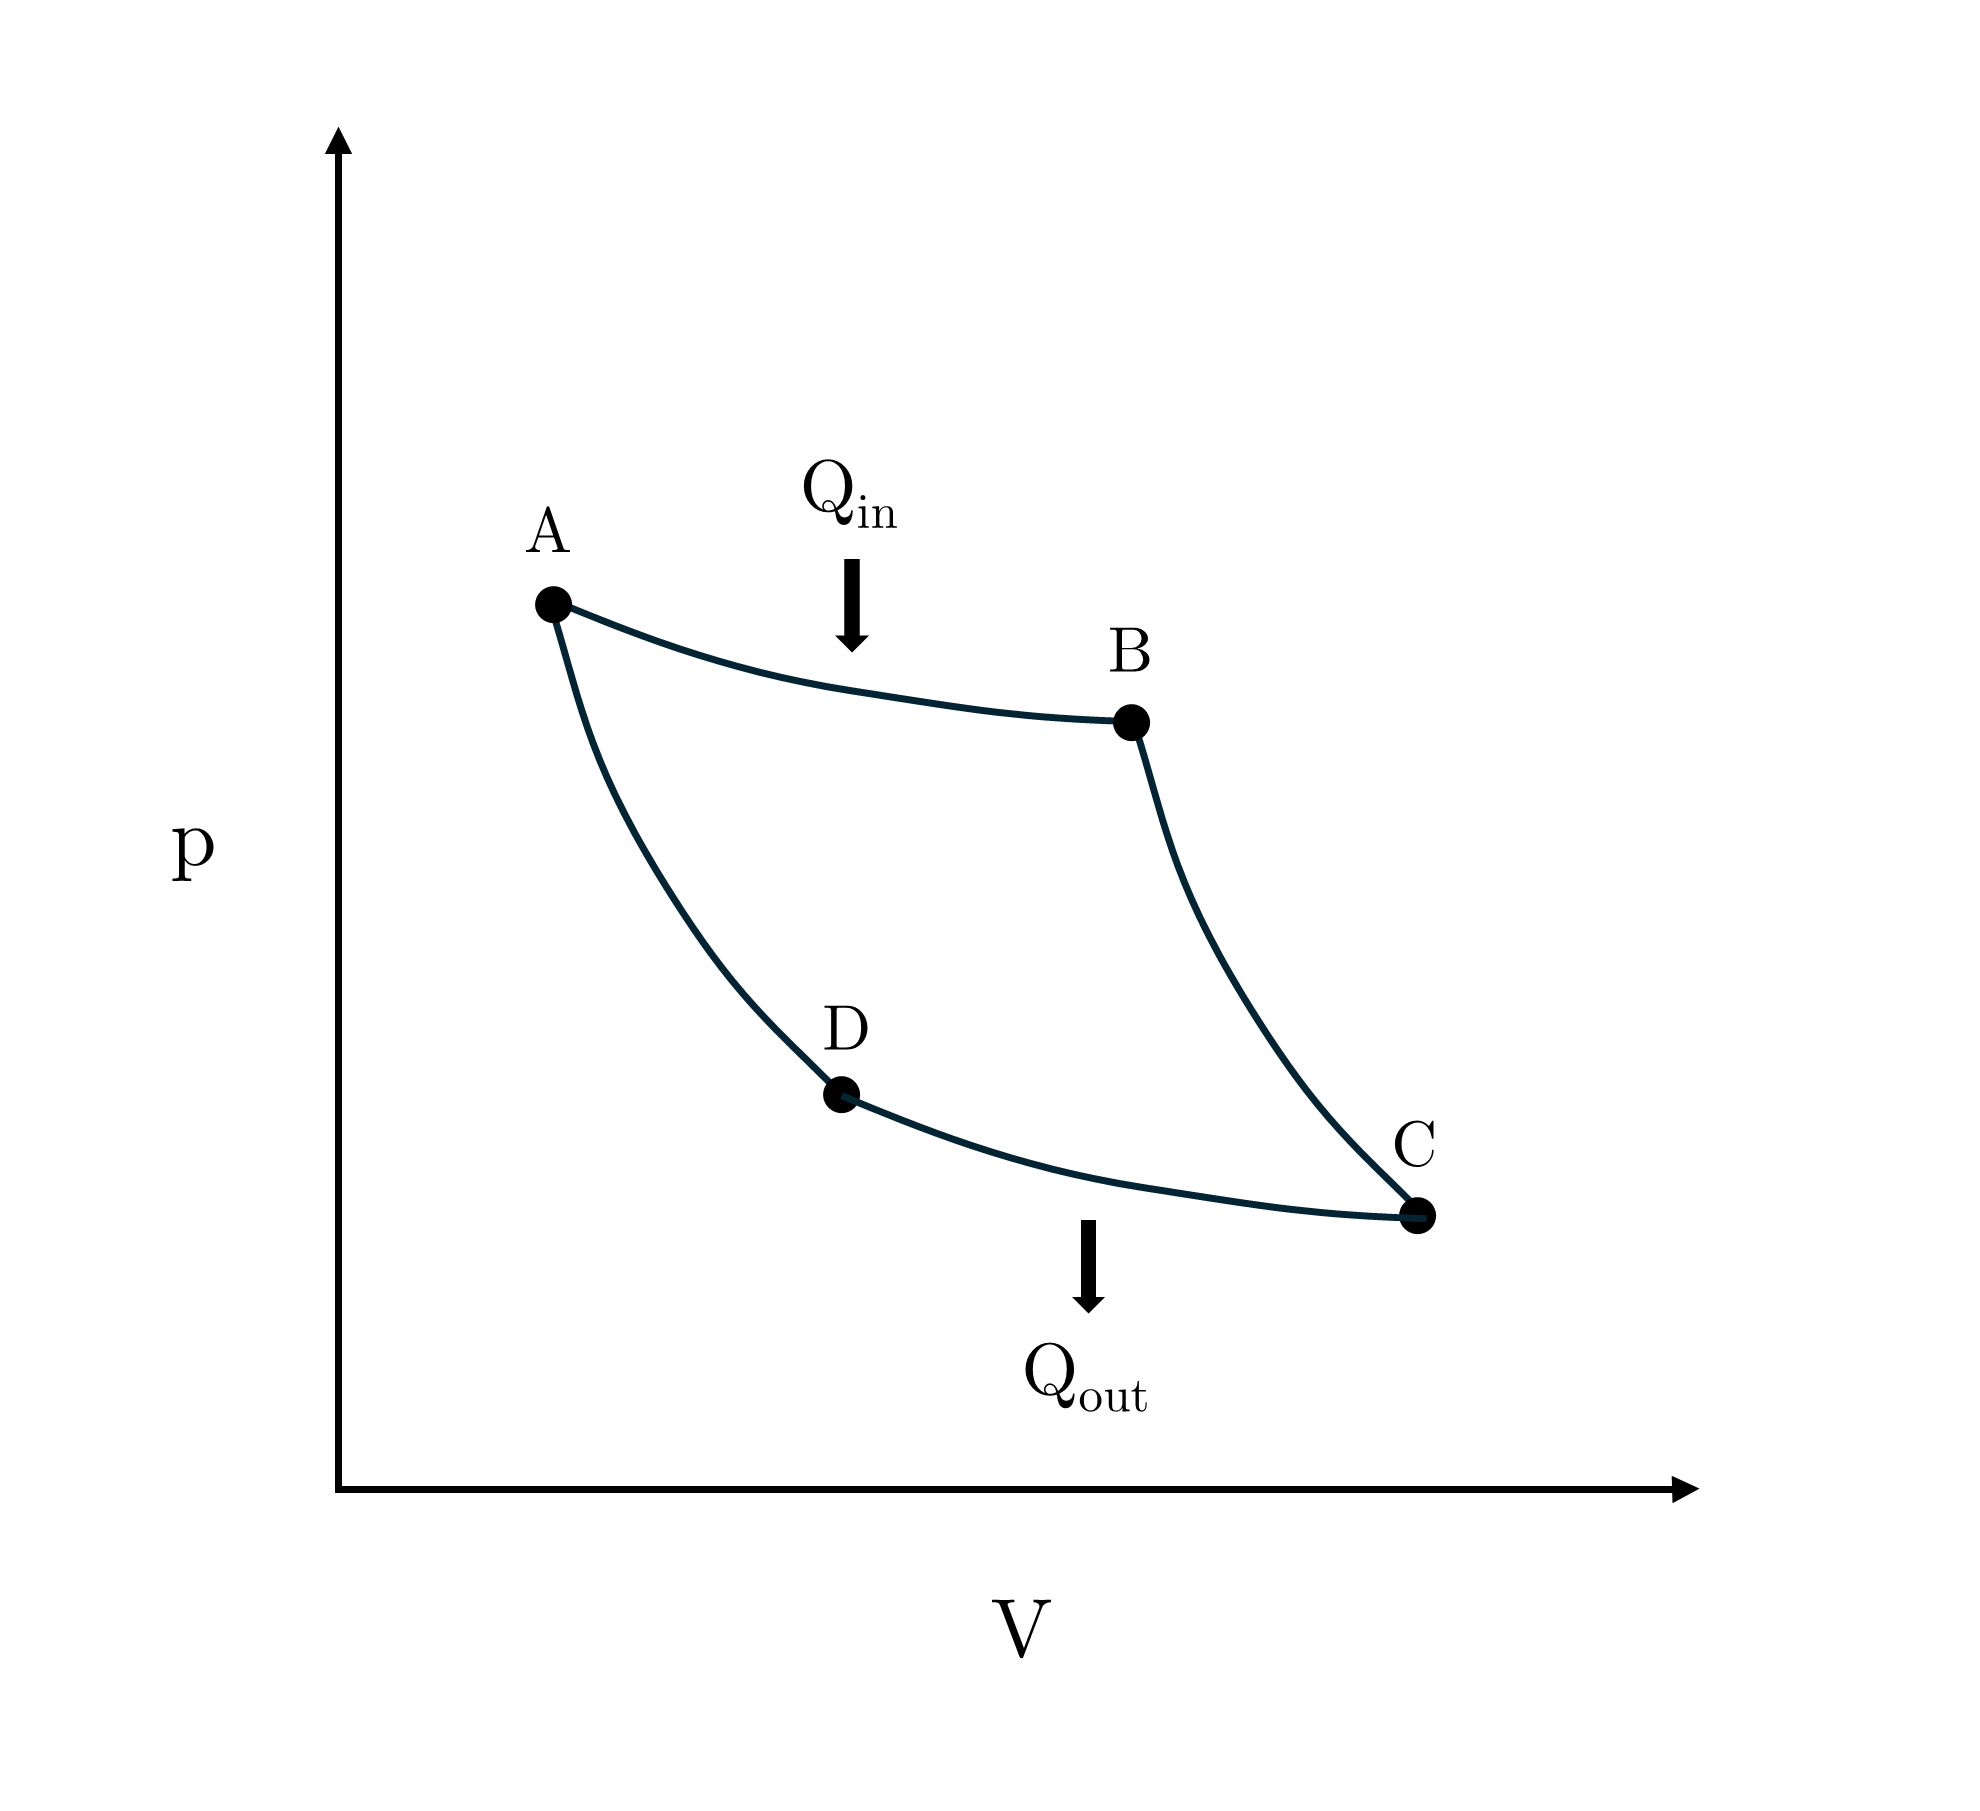
\includegraphics[width=0.6\textwidth]{Images/Classic Carnot Cycle.png}
%     \caption{Siklus Carnot pada bidang p,V. Siklus ini terdiri dari 4 segmen yang reversibel. \(AB\) adalah ekspansi isotermal, \(BC\) adalah ekspansi adiabatis, \(CD\) adalah kompresi isotermal, dan \(DA\) adalah kompresi adiabatis.}
%     \label{fig:ClassicCarnot}
% \end{figure}
% \noindent Semua proses yang terlibat adalah proses yang reversibel atau dapat diulang secara terus-menerus. Segmen \(AB\) adalah ekspansi isotermal di mana sejumlah panas \(Q_{in}\) ditarik masuk ke siklus dari sebuah sumber panas dengan termperatur tinggi \(T_{in}\). Segmen \(BC\) adalah ekspansi adiabatis di mana tidak ada panas yang keluar atau masuk. Segmen \(CD\) adalah kompresi isotermal di mana sejumlah panas \(Q_{out}\) dikeluarkan dari siklus ke pembuangan panas dengan termperatur \(T_{out}\). Terakhir segmen \(DA\) yang merupakan kompresi adiabatis. Jika efisiensi dari mesin ini dihitung, akan didapat,
% \begin{align}
%     \eta = \frac{W}{|Q_{in}|} = 1 - \frac{|Q_{out}|}{|Q_{in}|} = 1 - \frac{T_{out}}{T_{in}} \label{eq:CarnotEff}
% \end{align}
% Tanda absolut pada \(Q\) diberikan karena positif dan negatif dari \(Q\) hanya menentukan arah. Sedangkan efisiensi hanya memerlukan besarannya saja. Dari persamaan \ref{eq:CarnotEff} dapat diketahui bahwa efisiensi mesin panas tidak sampai 100\% kecuali jika temperatur pembuangan panasnya adalah 0 absolut yang mana dianggap mustahil. Bersamaan dengan hukum ke-2 termodinamika, efisiensi dari mesin Carnot memiliki konsekuesni lain yaitu mesin reversibel yang bekerja pada temperatur yang sama dengan mesin Carnot akan memiliki efisiensi yang sama dengan mesin Carnot. Sedangkan mesin tak reversibel yang bekerja pada temperatur yang lebih rendah dari mesin Carnot akan memiliki efisiensi yang lebih rendah dari mesin Carnot. \cite{Sekerka2015Thermal}
% \par Siklus yang relevan berikutnya adalah siklus Otto yang diberi nama sesuai dengan penemunya yaitu Nicolaus Otto (1832 - 1891). Seperti siklus Carnot, siklus Otto memiliki 4 proses dalam siklusnya. Namun, terdapat perbedaan proses dengan yang terjadi pada siklus Carnot. Beriktu adalah ilustrasi dari siklus Otto:
% \begin{figure} [H]
%     \centering
%     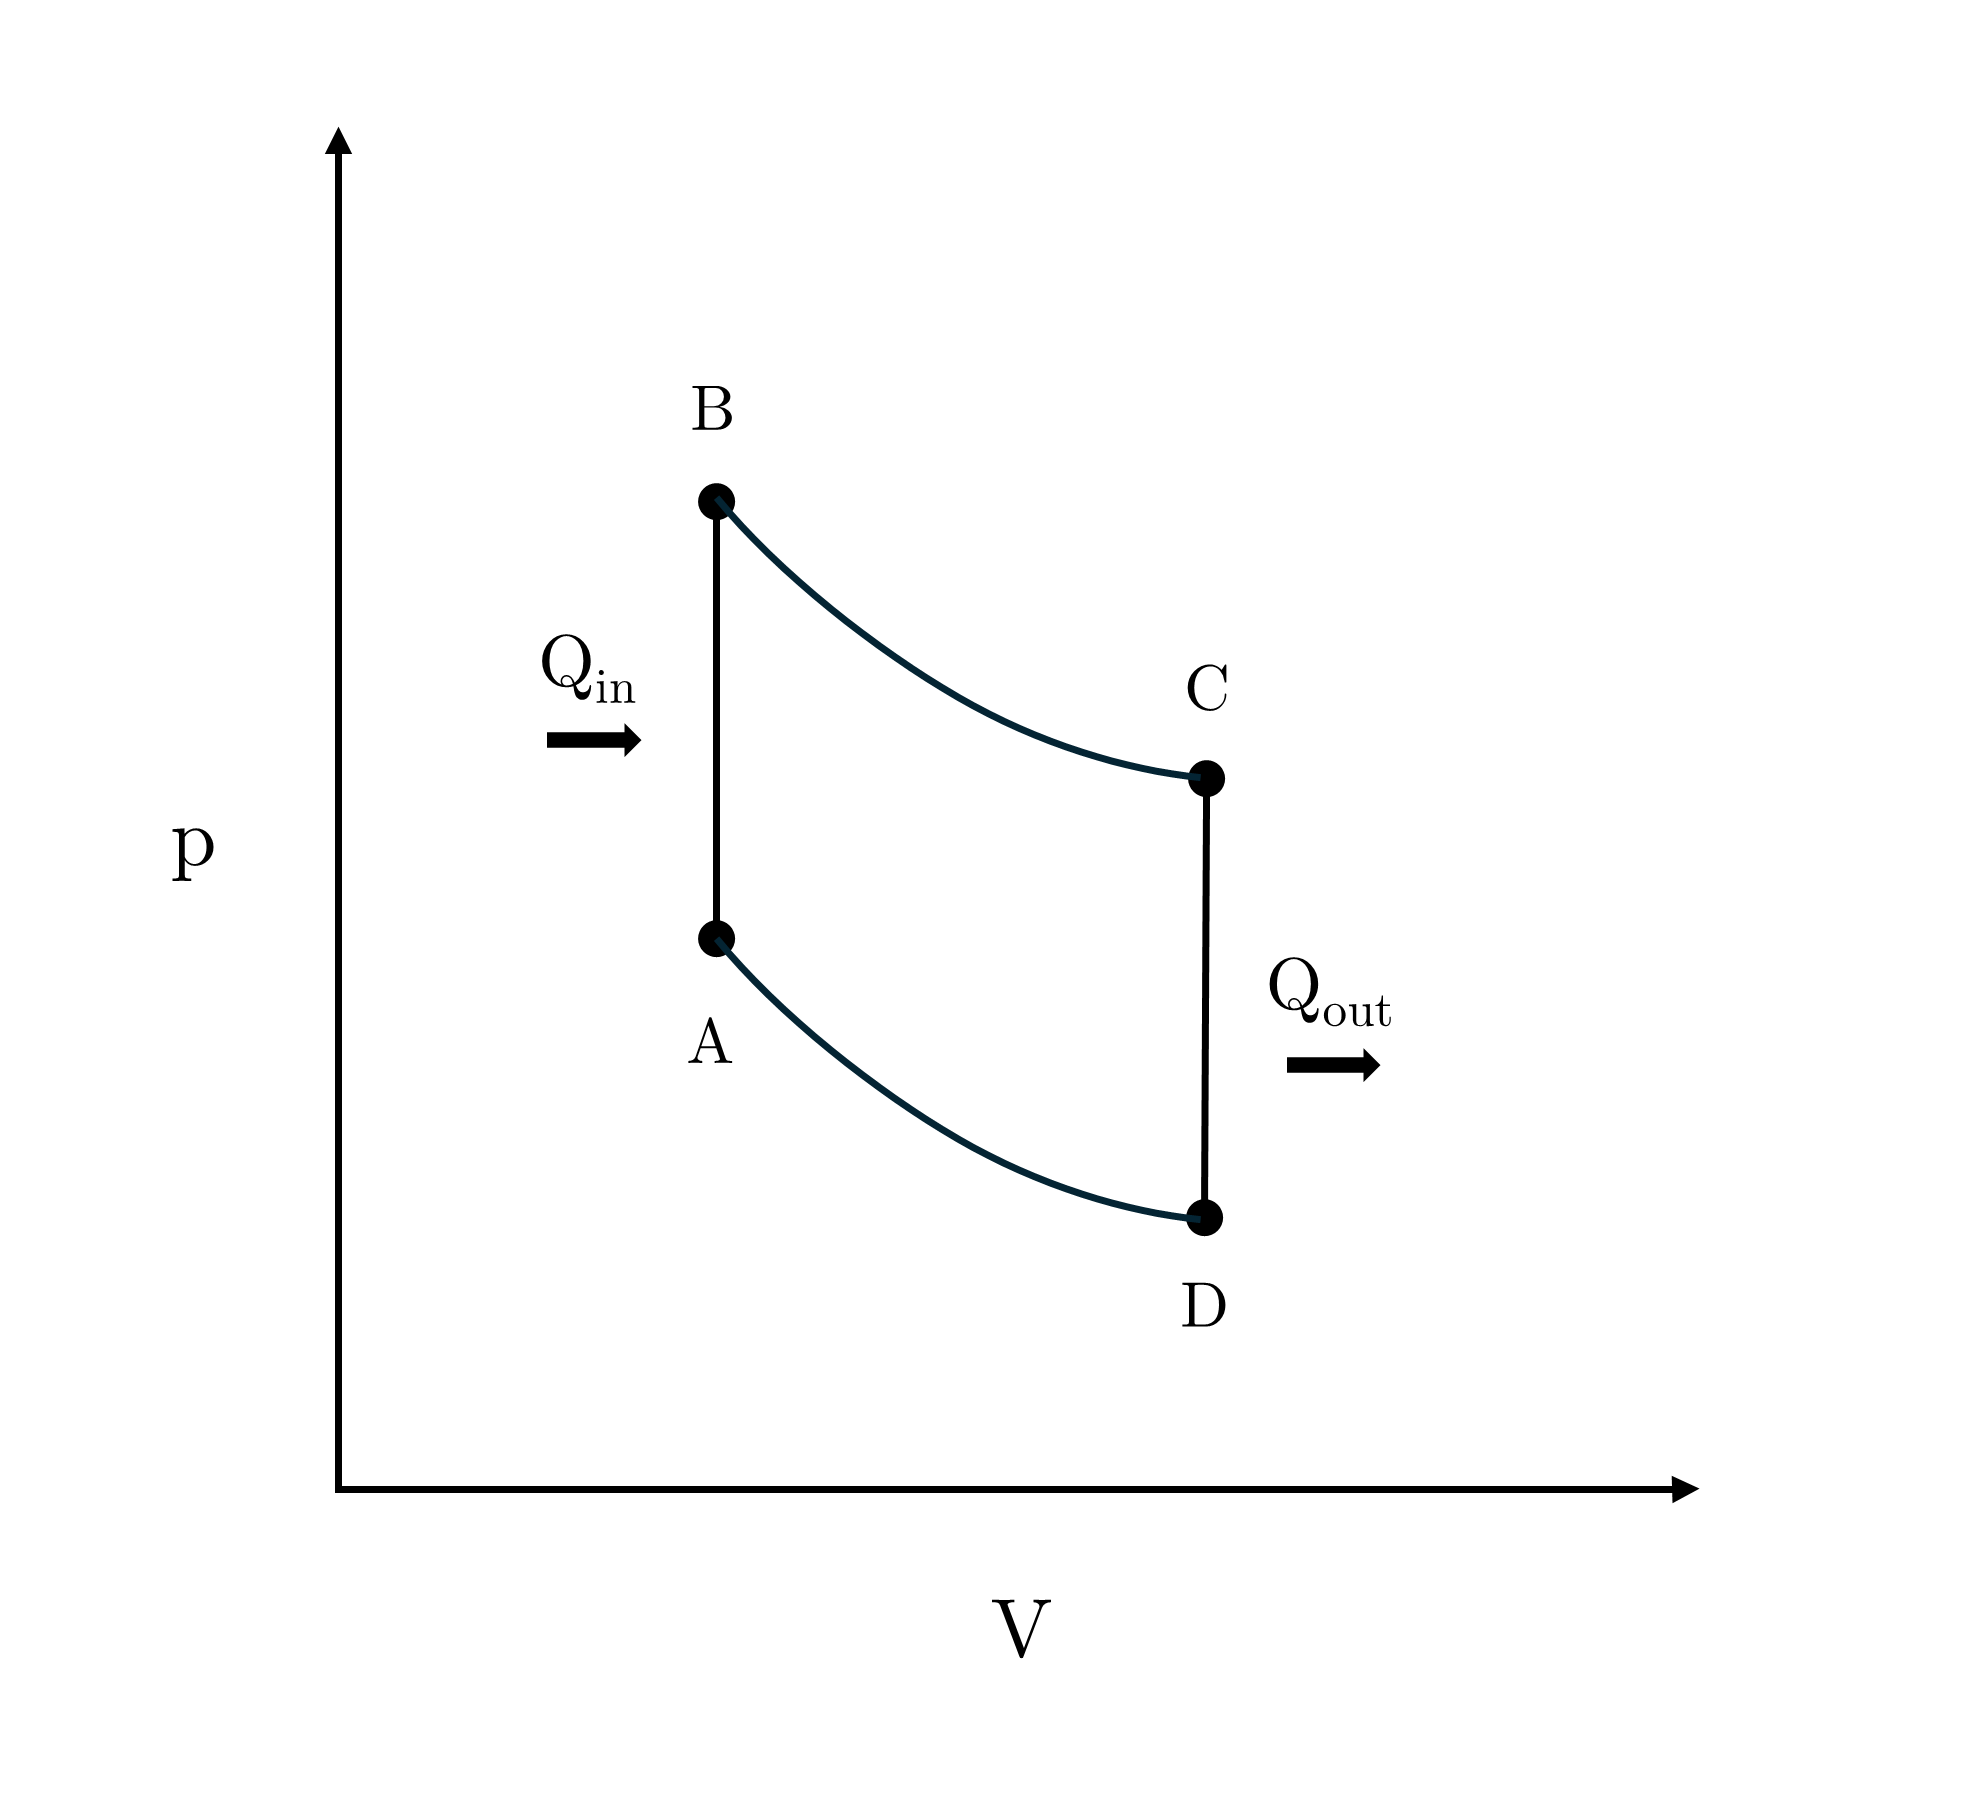
\includegraphics[width=0.6\textwidth]{Images/Classic Otto Cycle.png}
%     \caption{Siklus Otto pada bidang p,V. Siklus ini terdiri dari 4 segmen yang reversibel. \(AB\) adalah pembakaran isokorik, \(BC\) adalah ekspansi adiabatis, \(CD\) adalah pembuangan isokorik, dan \(DA\) adalah kompresi adiabatis.}
%     \label{fig:ClassicOtto}
% \end{figure}
% \noindent Pada siklus Carnot, panas masuk dengan temperatur yang konstan. Berbeda dengan siklus Otto di mana panas masuk tidak disertai dengan temperatur konstan, melainkan volume konstan. Secara praktis, proses masuknya panas adalah ketika proses pembakaran bahan bakar oleh busi pada mesin. Pada diagram, proses tersebut merupakan proses \(AB\). Proses \(BC\) dan \(DA\) sama seperti pada siklus Carnot yang merupakan proses ekspansi dan kompresi adiabatis. Terakhir \(CD\) yang merupakan proses pembuangan panas dengan volume konstan. Jika dilakukan perhitungan, efisiensi dari siklus Otto bisa didapatkan dengan bentuk,
% \begin{align}
%     \eta = 1 - \frac{T_D}{T_A}
% \end{align}
% Di mana \(T_D\) dan \(T_A\) merupakan temperatur pada titik \(D\) dan \(A\) pada diagram. Namun jika siklus bekerja pada basis standar udara dingin yang memiliki syarat utama kapasitas panas konstan dan perilaku gas ideal, bentuk dari efisiensi dapat diubah dengan menambahkan parameter baru.
% \begin{align}
%     \frac{T_A}{T_D} = \left(\frac{V_D}{V_A}\right)^{k-1} = r^{k-1}
% \end{align}
% Di mana \(k\) merupakan rasio kapasitas panas, \(k = c_p/c_v\). Dengan begitu, bentuk dari efisiensi berubah menjadi,
% \begin{align}
%     \eta = 1 - \frac{1}{r^{k-1}}
% \end{align}
% Hal ini membuat efisiensi menjadi fungsi dari rasio kompresi \(r\) dan rasio kapasitas panas \(k\). \cite{Moran2018Thermo}
% \par Siklus yang relevan terakhir adalah siklus Brayton yang pertama kali dikemukakan oleh George Brayton pada sekitar tahun 1870. Seperti siklus sebelumnya, siklus ini memiliki 4 proses namun dengan proses pembeda pada saat panas masuk dan keluar dari sistem. Siklus ini diilustrasikan sebagai berikut:
% \begin{figure} [H]
%     \centering
%     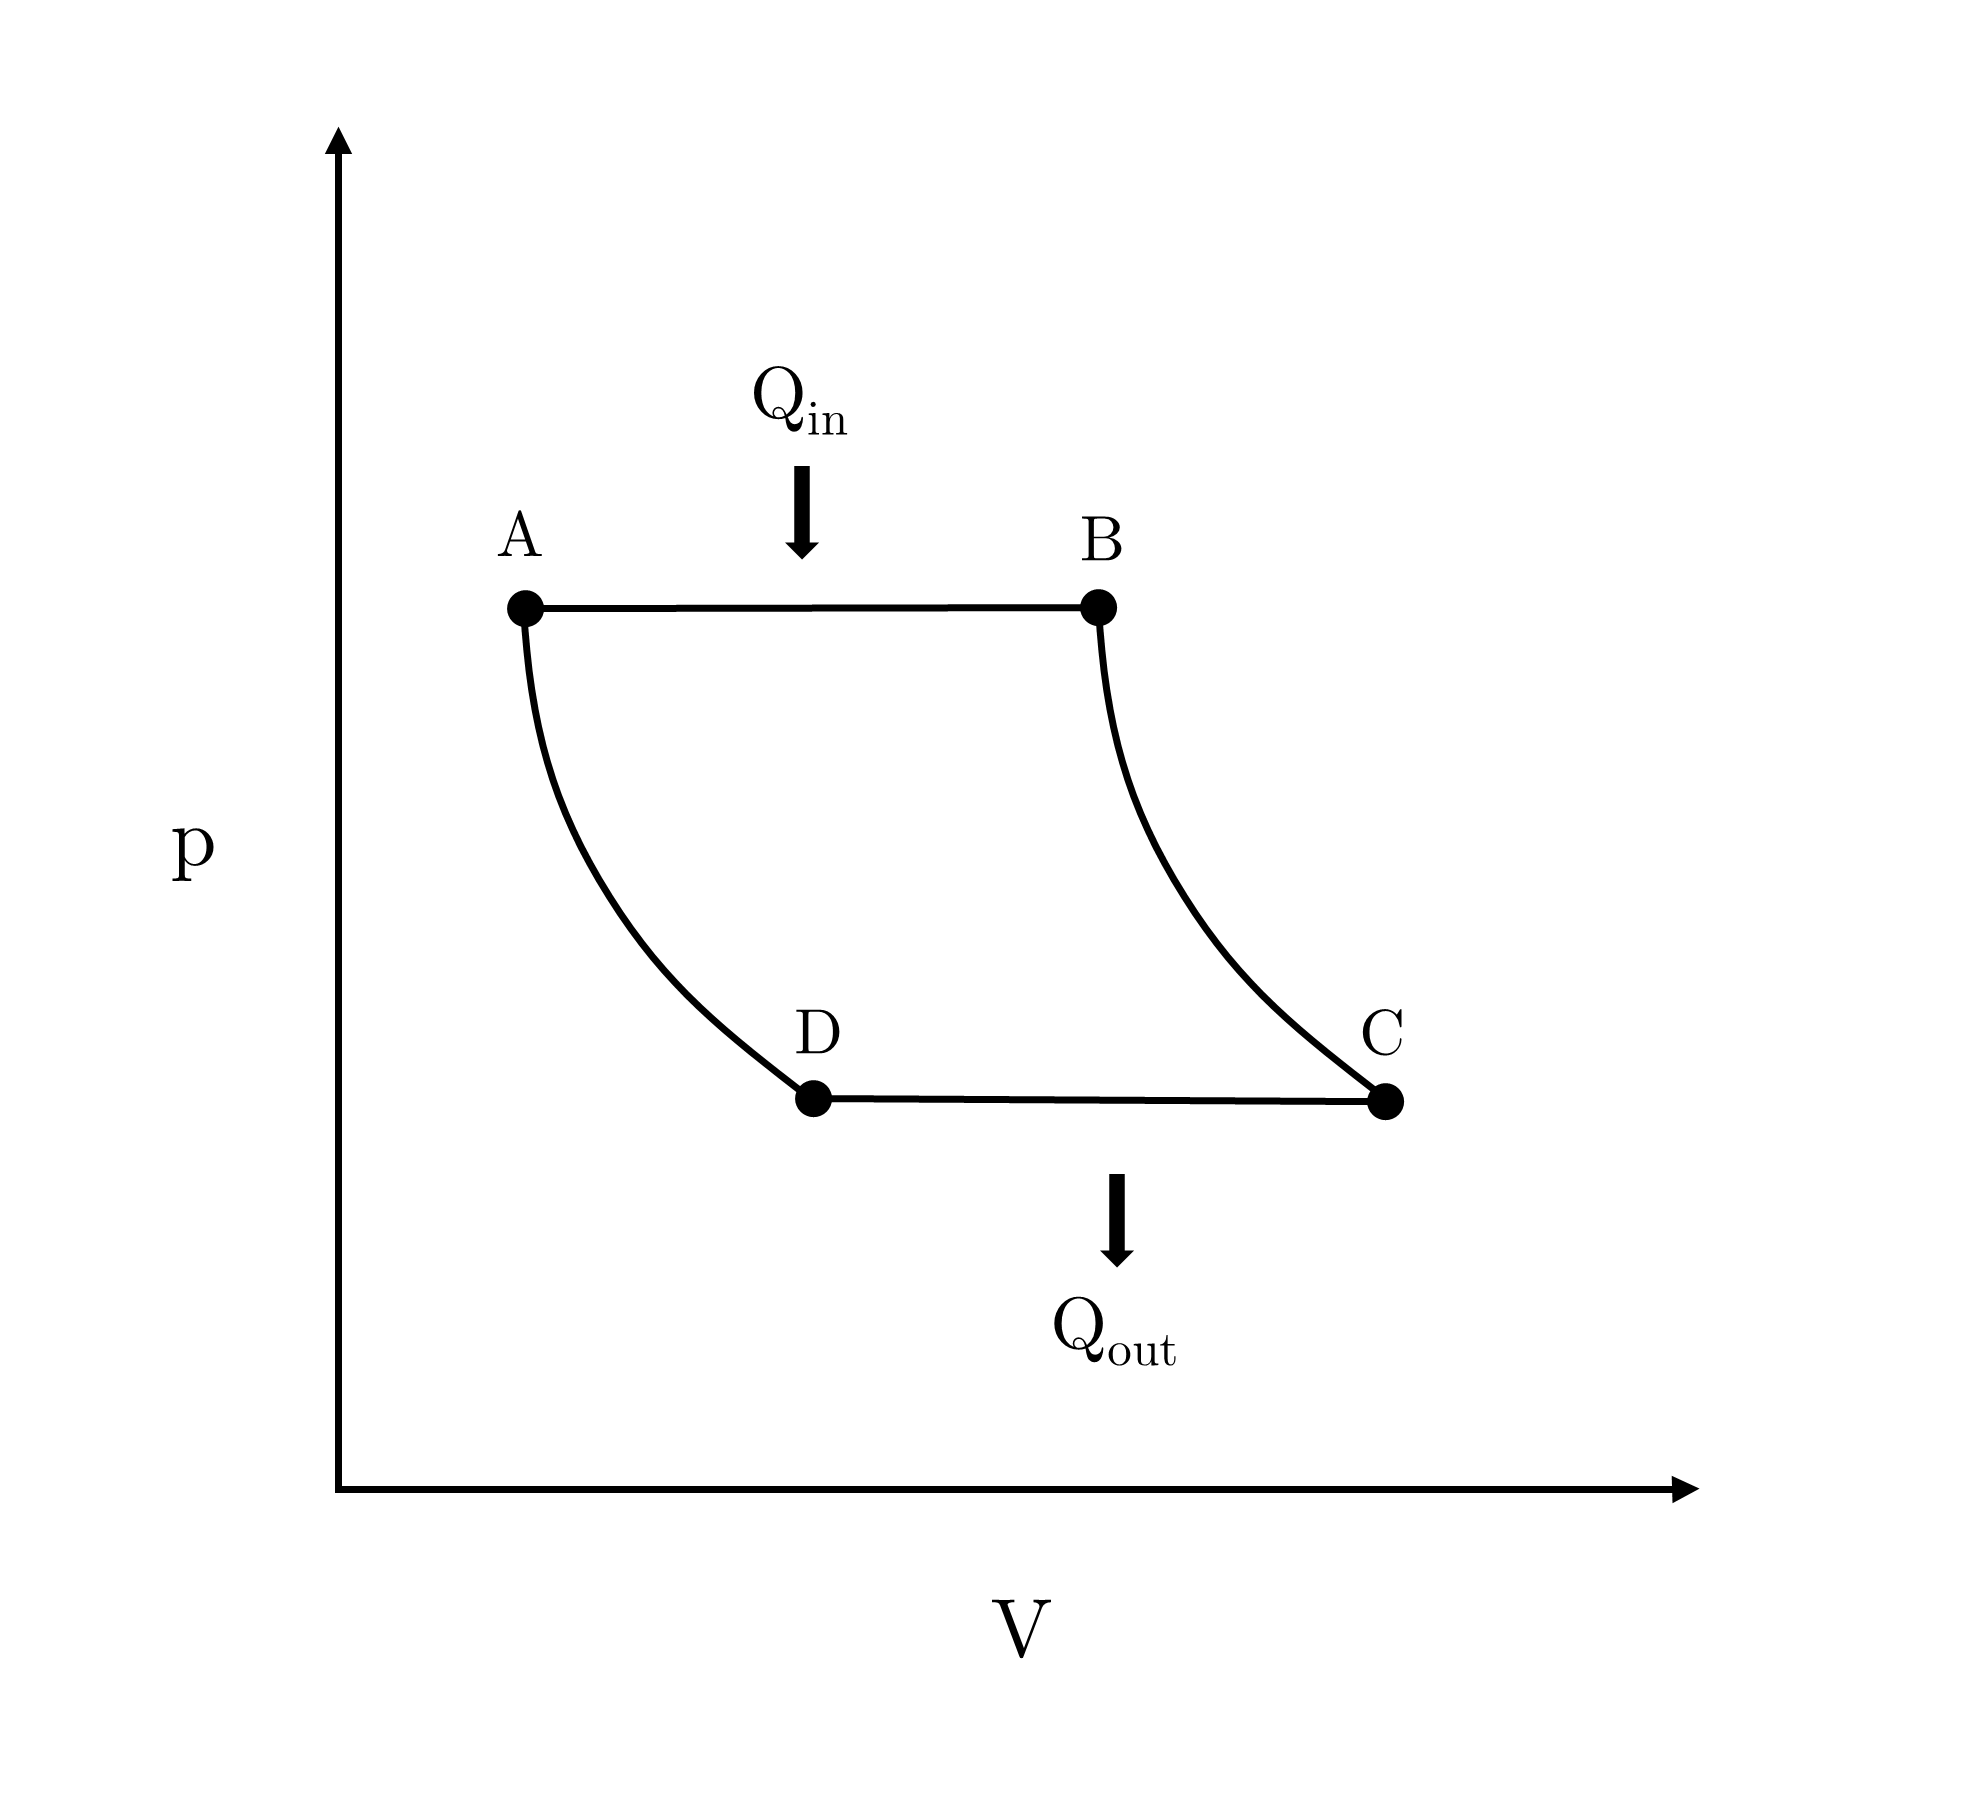
\includegraphics[width=0.6\textwidth]{Images/Classic Brayton Cycle.png}
%     \caption{Siklus Brayton pada bidang p,V. Siklus ini terdiri dari 4 segmen yang reversibel. \(AB\) adalah ekspansi isobarik, \(BC\) adalah ekspansi adiabatis, \(CD\) adalah kompresi isobarik, dan \(DA\) adalah kompresi adiabatis.}
%     \label{fig:ClassicBrayton}
% \end{figure}
% \noindent Tidak seperti siklus Carnot dan Otto, variabel yang konstan saat panas masuk ke siklus ini adalah tekanan \(p\). Pada praktisnya, siklus ini dikembangkan untuk membuat siklus terbuka pada turbin gas menjadi siklus tertutup di mana proses pembakaran diganti dengan penambahan panas dengan tekanan konstan. Jika melihat pada diagram, proses ini terjadi pada proses \(AB\) yang merupakan sebuah proses isobarik. Lalu, proses \(BC\) dan \(DA\) mirip seperti 2 siklus sebelumnya yang merupakan proses ekspansi dan kompresi adiabatik. Terakhir adalah proses \(CD\) yang merupakan pembuangan panas secara isobarik. Penggambaran diagram \ref{fig:ClassicBrayton} dibuat berdasarkan asumsi prosesnya terjadi secara stabil. Dengan begitu, efisiensi siklus Brayton dapat dihitung menggunakan asumsi standar udara dingin yang hasilnya dapat dinyatakan sebagai,
% \begin{align}
%     \eta = 1 - \frac{T_D(T_C/T_D - 1)}{T_A(T_B/T_A - 1)}
% \end{align}
% Bentuk dari efisiensi dapat diubah menjadi lebih sederhana dengan menambahkan rasio kapasitas panas \(k\) yang hubungannya dapat dinyatakan dengan,
% \begin{align}
%     \frac{T_A}{T_D} = \left(\frac{P_A}{P_D}\right)^\frac{k-1}{k} = \left(\frac{P_B}{P_C}\right)^\frac{k-1}{k} = \frac{T_B}{T_C}
% \end{align}
% Sehingga bentuk dari efisiensi berubah menjadi,
% \begin{align}
%     \eta = 1 - \frac{1}{r_p^\frac{k-1}{k}}
% \end{align}
% Di mana
% \begin{align}
%     r_p = \frac{P_A}{P_D}
% \end{align}
% Mirip seperti siklus Otto, persamaan tersebut membuat efisiensi menjadi fungsi dari rasio tekanan \(r_p\) dan rasio kapasitas panas \(k\). \cite{Yunus2024Thermo}
\par Salah satu tinjauan yang dibahas pada termodinamika kuantum adalah mesin panas kuantum. Sistem kuantum yang akan digunakan untuk mempelajari mesin panas kuantum adalah sistem partikel dalam sumur potensial tak-hingga 1 dimensi. Dalam konteksi ini, sumur dimodifikasi di mana salah satu tembok (yang kanan untuk kenyamanan) dapat bergerak dengan bebas untuk merepresentasikan piston serta memperbolehkan untuk terjadinya perubahan volume di dalam sistem. Hal ini dapat diilustrasikan sebagai berikut:
\begin{figure} [H]
    \centering
    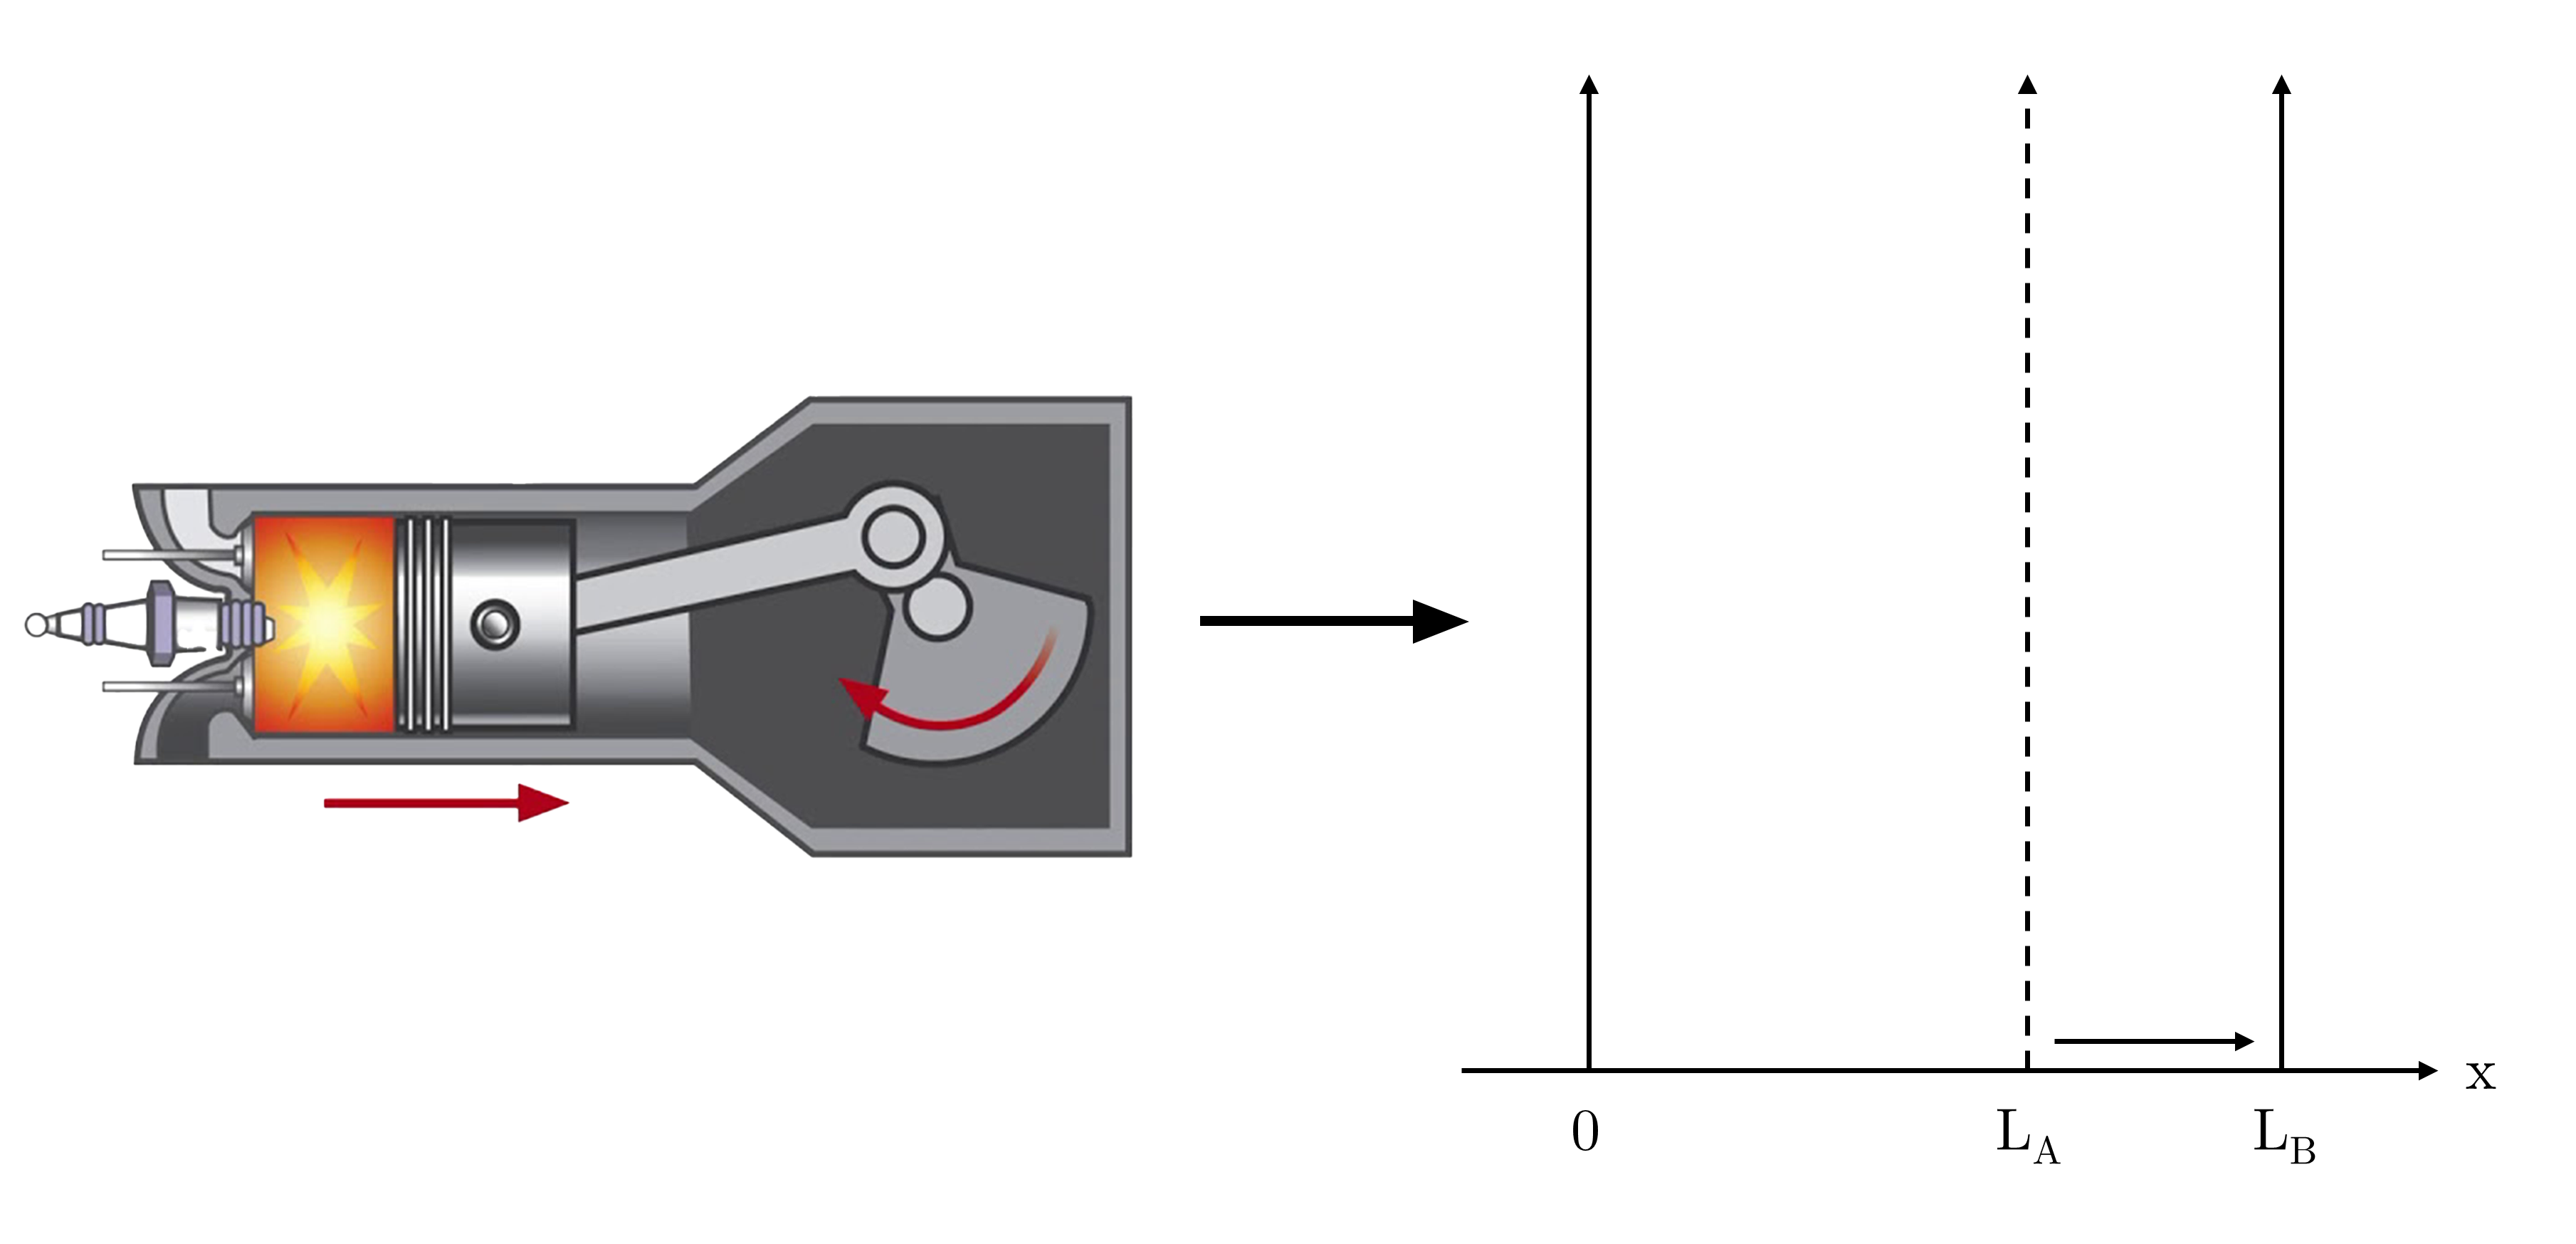
\includegraphics[width=0.6\textwidth]{Images/Piston & Movable Wall.png}
    \caption{Piston yang digantikan oleh potensial tak hingga dengan tembok kanan yang dapat bergerak dengan bebas. Diilustrasikan tembok bergerak dari \(L_A\) menuju \(L_B\). (Sumber gambar piston: \protect\cite{Toyota2017Pistons})}
    \label{fig:MovableWall}
\end{figure}
\noindent Perubahan lebar sumur ini tentunya akan merubah keadaan partikel yang berada di dalamnya. Konsekuensi dari hal ini juga akan berpengaruh terhadap proses-proses dalam siklus mesin panas kuantum \cite{Latifah2013QHE}. Urutan dari siklus yang akan dibahas adalah Carnot, Otto, dan Brayton. Pada tulisan ini, zat kerja yang ditinjau adalah 1 partikel yang terjebak dalam sumur potensial tak hingga dengan 2 keadaan; keadaan dasar dan keadaan tereksitasi pertama.

\subsection{Siklus Carnot Kuantum} Siklus Carnot terdiri dari 4 proses. Yaitu panas masuk melalui proses isotermal, lalu ekspansi adiabatik, kemudian panas keluar melalui proses isotermal, dan diakhiri dengan kompresi adiabatik. Namun, pada sistem kuantum proses isotermal dapat dikatakan juga sebagai proses isoenergetik karena temperatur merupakan representasi makro dari rerata energi partikel \cite{Purwanto2016QHE}. Gambaran proses dari siklus Carnot dapat diilustrasikan sebagai berikut:
\begin{figure} [H]
    \centering
    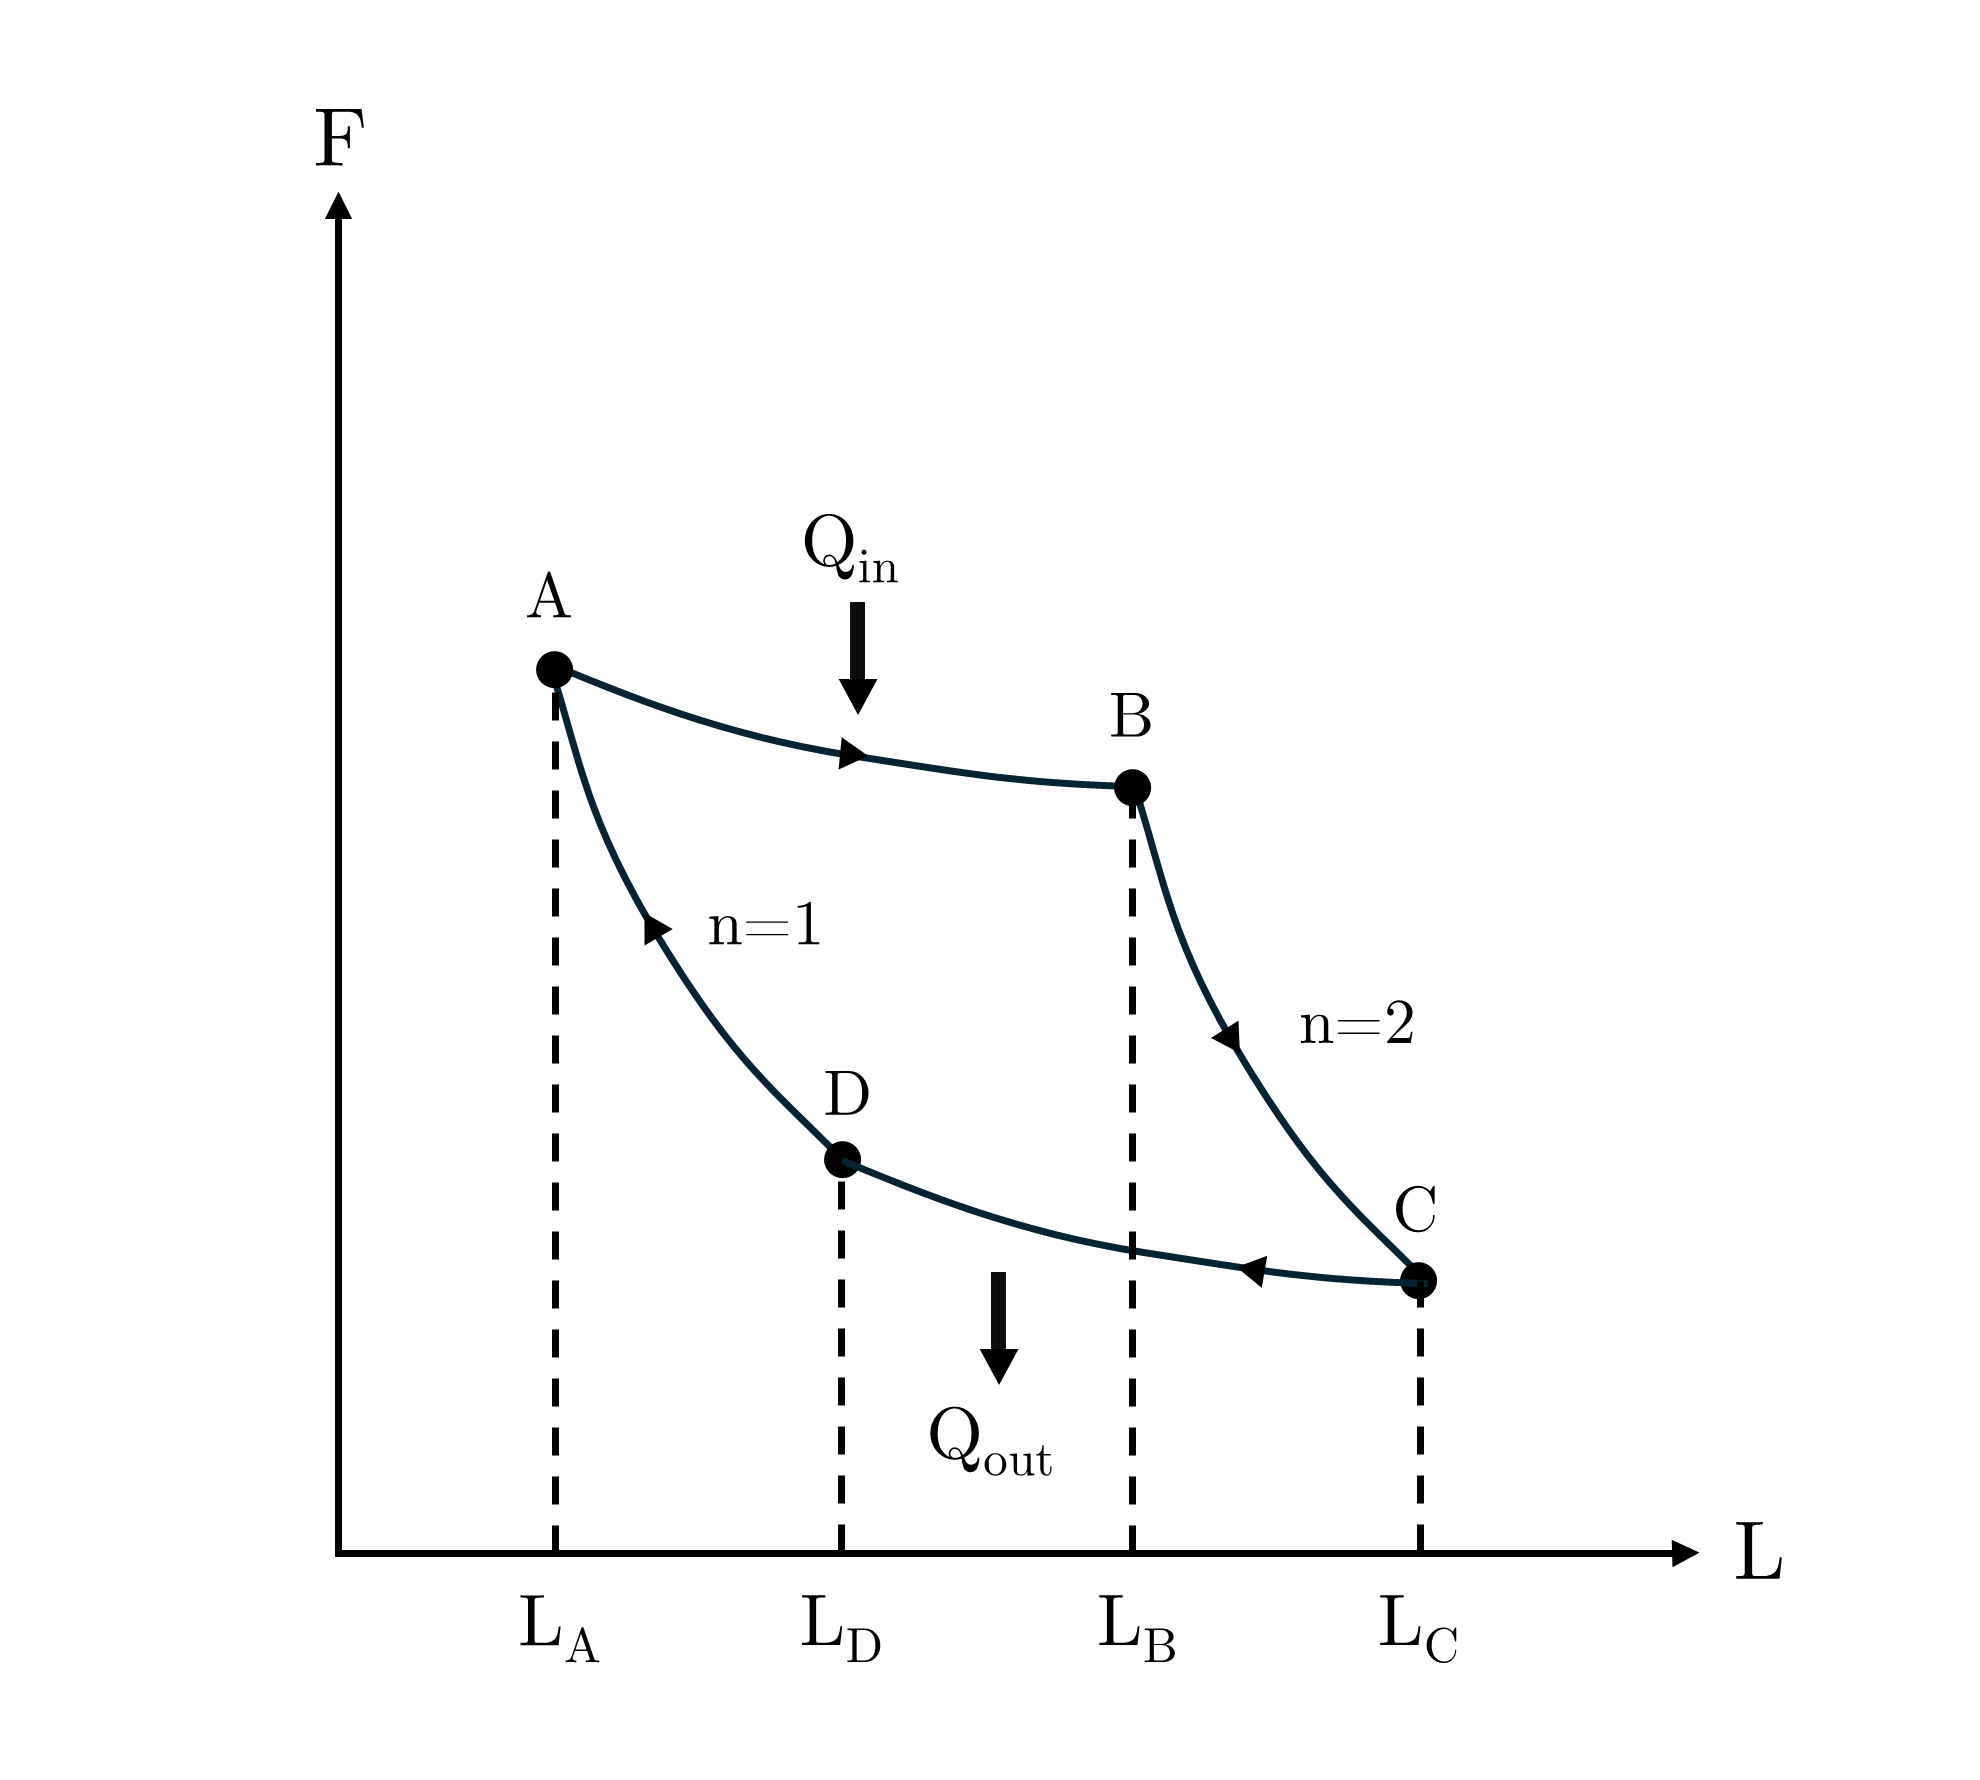
\includegraphics[width=0.5\textwidth]{Images/Quantum Carnot Cycle.png}
    \caption{Siklus Carnot pada bidang F,L. Siklus ini terdiri dari 4 segmen yang reversibel. \(AB\) adalah ekspansi isoenergetik, \(BC\) adalah ekspansi adiabatis, \(CD\) adalah kompresi isotermal, dan \(DA\) adalah kompresi adiabatis. \protect\cite{Bender2000Quantum}}
    \label{fig:QCarnotCycle}
\end{figure}
Keadaan awal pada titik \(A\) dari siklus ini dan semua siklus yang ditinjau adalah keadaan dasar (\(n=1\)). Siklus ini dibuka dengan segmen \(AB\) di mana panas masuk ke sistem secara isoenergetik atau dapat ditulis \(E_{AB}(L) = E_1(L_A) = E_2(L_B)\). Tembok kanan bergerak dari \(L_A\) ke \(L_B\). Tingkatan energi pada proses ini berubah tanpa mengubah rerata energi partikel. Sehingga, bentuk persamaannya dapat dipilih antara tingkat energi pada \(L_A\) ataupun \(L_B\). Di sini, diambil bentuk energi pada \(L_A\). Sehingga rerata energi saat panas masuk dapat ditulis sebagai:
\begin{align}
    E(L_A) = \frac{\hbar^2\pi^2}{2mL_A^2}
    \label{eq:CarnotE_AB}
\end{align}
Menggunakan persamaan \ref{eq:CarnotE_AB} dan \ref{eq:QuantumU} dapat diketahui hubungan antara panjang sumur dan probabilitas.
\begin{align}
    % \langle E_{AB} \rangle &= \Sigma E_n P_n \\
    % &= E_1(L)P_1(L) + E_2(L)P_2(L) \\
    % \frac{\hbar^2\pi^2}{2mL_A^2} &= \frac{\hbar^2\pi^2}{2mL^2} P_1(L) + \frac{\hbar^2\pi^2}{2mL^2} \cdot 4P_2(L) \\
    % \frac{1}{L_A^2} &= \frac{P_1(L) + 4P_2(L)}{L^2} \\
    \frac{L^2}{L_A^2} &= P_1(L) + 4P_2(L) \label{eq:RegCarnotLtoP}
\end{align}
Dengan \(P_1(L) + P_2(L) = 1\) yang berlaku juga untuk seluruh siklus yang ditinjau pada tulisan ini. Selain itu, dari konstannya rerata energi ini, dapat diketahui juga hubungan lebar sumur \(L_B = 2L_A\). Hubungan-hubungan tersebut dapat digunakan untuk mencari besaran panas yang masuk melalui gaya yang dialami oleh tembok bergerak. Gaya didefinisikan sebagai negatif turunan pertama dari energi eigen partikel. Secara matematis dapat ditulis sebagai berikut:
% \begin{align}
%     E_{AB} &= E_1(L_A) = E_2(L_B) \\
%     \frac{\hbar^2\pi^2}{2mL_A^2} &= \frac{\hbar^2\pi^2}{2mL_B^2} \cdot 4 \\
%     L_B &= 2L_A
% \end{align}
\begin{align}
    F = -\frac{d}{dL}E_n(L) = \frac{\hbar^2\pi^2}{mL^3}n^2 \label{eq:RegCarnotF}
    % &= -\frac{d}{dL} \frac{\hbar^2\pi^2}{2mL^2}n^2 \\
    % F &= \frac{\hbar^2\pi^2}{mL^3}n^2
\end{align}
Sedangkan gaya selama proses berlangsung merupakan penjumlahan gaya kali probabilitas untuk semua tingkat energi yang diizinkan yang dapat ditulis sebagai \(F_{AB}(L) = \Sigma F(L)P_n(L)\). Pada proses panas masuk, besaran ini dapat ditulis sebagai,
\begin{align}
    F_{AB}(L) = \frac{\hbar^2\pi^2}{mL_A^2L} \label{eq:RegCarnotFab}
    % F_{AB} &= \Sigma F(L)P_n(L) \\
    % &= \frac{\hbar^2\pi^2}{mL^3} \cdot P_1(L) + \frac{\hbar^2\pi^2}{mL^3} \cdot 4P_2(L) \\
    % &= \frac{\hbar^2\pi^2}{mL^3}(P_1(L) + 4P_2(L)) \\
\end{align}
Dari gaya tersebut, panas yang masuk dapat diketahui. Besaran panas ini didefinisikan sebagai,
\begin{align}
    Q_{AB} = \int_{L_A}^{L_B}F_{AB}(L)dL + \dot{Q_r}\tau
    % &= \frac{\hbar^2\pi^2}{mL_A^2}\ln{\frac{L_B}{L_A}} + \dot{Q_r}\tau \\
\end{align}
Dengan substitusi persamaan (\ref{eq:RegCarnotFab}) diperoleh
\begin{align}
    Q_{AB} = \frac{\hbar^2\pi^2}{mL_A^2}\ln{2} + \dot{Q_r}\tau \label{eq:RegCarnotQab}
\end{align}
Di mana \(\dot{Q_r}\) merupakan disipasi panas. Hal ini terjadi karena reservoir panas dan dingin dianggap berukuran sangat besar sehingga menimbulkan kebocoran panas. Sedangkan \(\tau\) merupakan total waktu selama 1 siklus. \cite{Wu2006Brayton}
\par Proses dilanjutkan pada segmen \(BC\) dengan ekspansi isoentropis di mana tidak ada panas yang keluar masuk dan entropi berada pada keadaan konstan. Tembok bergerak lagi dari \(L_B\) ke \(L_C\). Tidak seperti sebelumnya, tingkatan energi pada proses ini tidak berubah. Kemudian proses berlanjut pada segmen \(CD\) dengan kompresi isoenergetik di mana panas dibuang dari sistem. Tembok bergerak dari \(L_C\) ke \(L_D\) lalu tingkatan energi eigen pada proses ini turun kembali ke keadaan dasar tanpa merubah rerata energinya, yang mana pada proses ini ditulis sebagai
\begin{align}
    E(L_C) = \frac{\hbar^2\pi^2}{2mL_C^2} \cdot 4
\end{align}
Seperti pada saat panas masuk, rerata energi ini dapat digunakan untuk mencari hubungan antar probabilitas dan panjang sumur.
\begin{align}
    % \langle E_{CD} \rangle &= E_1(L)P_1(L) + E_2(L)P_2(L) \\
    % \frac{\hbar^2\pi^2}{2mL_C^2} \cdot 4 &= \frac{\hbar^2\pi^2}{2mL^2}P_1(L) + \frac{\hbar^2\pi^2}{2mL^2} \cdot 4P_2(L) \\
    % \frac{4}{L_C^2} &= \frac{P_1(L) + 4P_2(L)}{L^2} \\
    \frac{4L^2}{L_C^2} &= P_1(L) + 4P_2(L)
\end{align}
Hubungan tersebut digunakan untuk mencari besaran gaya yang dialami oleh tembok selama proses ini.
\begin{align}
    F_{CD}(L) = \frac{4\hbar^2\pi^2}{mL_C^2 L} \label{eq:RegCarnotFcd}
    % &= \frac{\hbar^2\pi^2}{mL^3}(P_1(L) + 4P_2(L)) \\
\end{align}
Karena rerata energi konstan saat panas keluar, didapatkan hubungan panjang tembok \(L_D = \frac{1}{2}L_C\). Sehingga besaran dari panas yang keluar sistem dapat dihitung. 
\begin{align}
    Q_{CD} &= \left| \int_{L_C}^{L_D} F_{CD}(L)dL \right| + \dot{Q_r}\tau
\end{align}
Dengan subsitutsi persamaan (\ref{eq:RegCarnotFcd}) didapat
\begin{align}
    Q_{CD} &= \frac{4\hbar^2\pi^2}{mL_C^2}\ln{2} + \dot{Q_r}\tau
\end{align}
Setelah itu proses diakhiri dengan kompresi isoentropis pada segmen \(DA\) di mana tembok bergerak tanpa mengubah tingkatan energi eigennya. 
\par Besaran-besaran di atas selanjutnya digunakan untuk mencari \textit{power output} dan efisiensi. Untuk itu, diperlukan kerja dalam 1 siklus. Di sini, dianggap \(W_{BC}-W_{DA}=0\) \cite{LibreTexts2021Carnot}. Dengan begitu, didapatkan kuantitas kerja sebagai berikut:
\begin{align}
    W = Q_{AB} - Q_{CD} = \frac{\hbar^2\pi^2}{m}\left(\frac{1}{L_A^2} - \frac{4}{L_C^2}\right) \ln{2}
    % &= \frac{\hbar^2\pi^2}{mL_A^2}\ln{2} + \dot{Q_r}\tau - \left(\frac{4\hbar^2\pi^2}{mL_C^2}\ln{2} + \dot{Q_r}\tau \right) \\
\end{align}
Misal digunakan sebuah parameter ekspansi yang didefinisikan sebagai \(L_C = rL_A\). Maka bentuk persamaan kerja menjadi
\begin{align}
    W = \frac{\hbar^2\pi^2}{m}\left(\frac{r^2-4}{L_C^2}\right)\ln{2} \label{eq:RegCarnotW}
    % &= \frac{\hbar^2\pi^2}{m}\left(\frac{L_C^2}{L_A^2 L_C^2} - \frac{4}{L_C^2}\right)\ln{2} \\
\end{align}
Menggunakan persamaan tersebut, \textit{power output} dapat dihitung. Namun, terdapat 1 variabel yang masih belum diketahui, yaitu \(\tau\). Variabel ini dapat didefinisikan sebagai total gerak \(L_0\) dibagi kecepatan rata-rata \(\overline{\nu}\). Dari Gambar \ref{fig:QCarnotCycle}, total gerak yang dilakukan selama 1 siklus adalah \(L_0 = 2(L_C - L_A)\). Sehingga waktu total selama 1 siklus \(\tau\) dapat dituliskan sebagai,
% \begin{align}
%     % L_0 &= (L_B - L_A) + (L_C - L_B) - (L_D - L_C) - (L_A - L_D) \\
%     L_0 &= 2(L_C - L_A)
% \end{align}
\begin{align}
    \tau = \frac{L_0}{\overline{\nu}} = \frac{2(L_C - L_A)}{\overline{\nu}} \label{eq:TauDef}
\end{align}
Dengan menggunakan persamaan (\ref{eq:RegCarnotW}) dan (\ref{eq:TauDef}), besaran \textit{power output} dapat dituliskan sebagai berikut:
\begin{align}
    P = \frac{W}{\tau} = \frac{\hbar^2\pi^2\overline{\nu}}{2mL_A^3}\left(\frac{r^2 - 4}{r^3 - r^2}\right)\ln{2}
    % &= \frac{\hbar^2\pi^2}{m}\left(\frac{r^2 - 4}{L_C^2}\right)\ln{2} \cdot \frac{\overline{\nu}}{2(L_C - L_A)} \\
    % &= \frac{\hbar^2\pi^2\overline{\nu}}{2m}\left(\frac{r^2 - 4}{L_C^3 - L_C^2 L_A}\right)\ln{2} \\
\end{align}
Di sini, \textit{power output} dibuat tak berdimensi dan hanya sebagai fungsi dari \(r\). \textit{Power output} tanpa dimensi ini dituliskan sebagai,
\begin{align}
    P^* = \frac{W}{A\tau} = \frac{\ln{2}}{2}\left(\frac{r^2 - 4}{r^3 - r^2}\right)
\end{align}
Dengan \(A = \hbar^2\pi^2\overline{\nu}/mL_A^3\). Selanjutnya efisiensi yang didapatkan menggunakan persamaan (\ref{eq:RegCarnotQab}) dan (\ref{eq:RegCarnotW}) sebagai berikut:
\begin{align}
    \eta = \frac{W}{Q_{AB}} = \frac{\frac{\hbar^2\pi^2}{m}\left(\frac{r^2 - 4}{L_C^2}\right)\ln{2}}{\frac{\hbar^2\pi^2}{mL_A^2}\ln{2} + \frac{2\dot{Q_r}(L_C - L_A)}{\overline{\nu}}}
    % &= \frac{\frac{\hbar^2\pi^2}{m}\left(\frac{r^2 - 4}{L_C^2}\right)\ln{2}}{\frac{\hbar^2\pi^2}{mL_A^2}\ln{2} + \dot{Q_r}\tau} \\
\end{align}
Dengan melihat dimensi dari \textit{power output} dan untuk menyederhanakan perhitungan, diasumsikan aliran panas yang bocor memiliki bentuk sebagai berikut:
\begin{align}
    \dot{Q_r} = \beta\frac{\hbar^2\pi^2\overline{\nu}}{2mL_A^3}\ln{2}
\end{align}
Di mana \(\beta\) disebut parameter disipasi dan merupakan sebuah konstanta. Jika demikian, maka efisiensi dari siklus Carnot ini adalah,
\begin{align}
    % \eta &= \frac{\frac{\hbar^2\pi^2}{m}\left(\frac{r^2 - 4}{L_C^2}\right)\ln{2}}{\left(\frac{\hbar^2\pi^2}{mL_A^2}\ln{2} + \frac{2(L_C - L_A)}{\overline{\nu}} \cdot \beta\frac{\hbar^2\pi^2\overline{\nu}}{2mL_A^3}\ln{2}\right)} \\
    % &= \frac{r^2-4}{r^2(1 + \beta(r-1))} \\
    \eta &= \frac{1 - \left(\frac{2}{r}\right)^2}{1 + \beta(r-1)}
\end{align}
Yang mana membuat efisiensi menjadi fungsi dari \(r\) saja. Dengan pengaturan seperti itu, untuk memastikan nilai efisiensi positif, jelas bahwa nilai \(r\) haruslah lebih dari 2.
\par Dari kuantitas yang sudah didapat, dapat dibuat 3 grafik untuk menggambarkan pengaruh parameter \(r\) dan \(\beta\) terhadap \textit{power output} serta efisiensi dari siklus Carnot kuantum ini. Pertama adalah grafik \textit{power output} tak berdimensi \(P^*\) terhadap \(r\),
\begin{figure} [H]
    \centering
    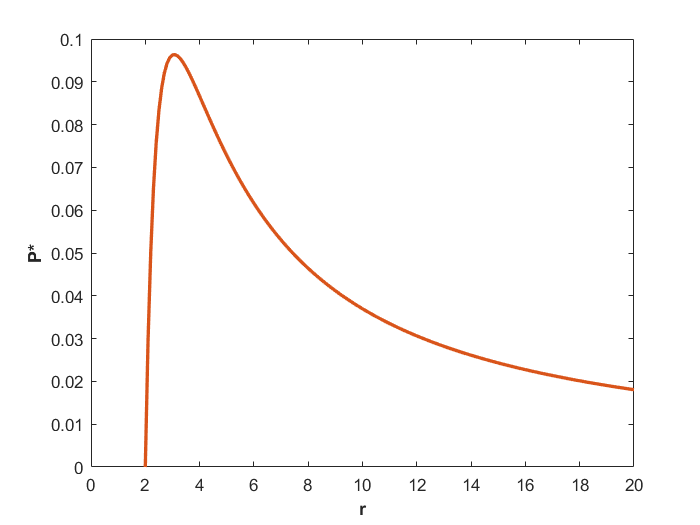
\includegraphics[width=0.6\textwidth]{Images/Ordinary Carnot P vs r.png}
    \caption{\textit{power output} tak berdimensi \(P^*\) terhadap \(r\) pada siklus Carnot kuantum.}
    \label{fig:OrdinaryCarnotPvsR}
\end{figure}
\noindent Pada grafik tersebut dapat dilihat bahwa nilai \textit{power output} yang real positif dimulai dari \(r=2\). Selanjutnya meningkat tajam dan terdapat titik balik di sekitar \(r=3.1\). Setelah itu \textit{power output} terus menurun dan ujungnya adalah konvergensi di \(P^*=0\) di \(r\rightarrow+\infty\). Grafik berikutnya adalah efisiensi \(\eta\) terhadap \(r\).
\begin{figure} [H]
    \centering
    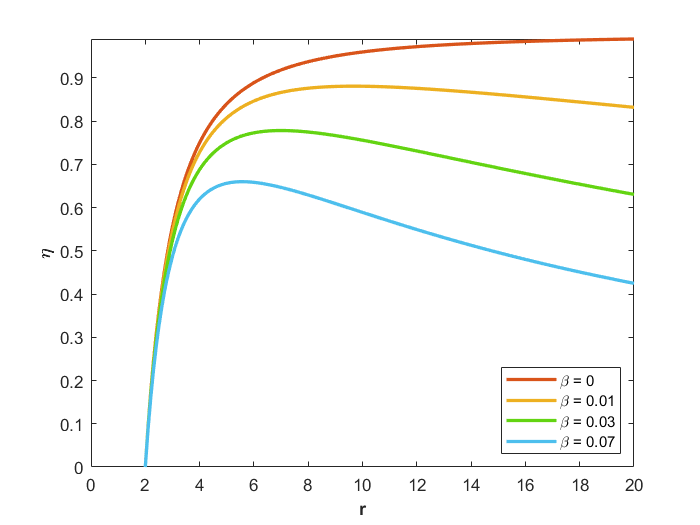
\includegraphics[width=0.6\textwidth]{Images/Ordinary Carnot Eta vs r.png}
    \caption{Efisiensi \(\eta\) terhadap \(r\) pada siklus Carnot kuantum dengan variasi pada nilai \(\beta\).}
    \label{fig:OrdinaryCarnotEtavsR}
\end{figure}
\noindent Pada keadaan tanpa disipasi (\(\beta=0\)), nilai efisiensi akan bisa mencapai nilai \(\eta=1\) pada \(r\rightarrow+\infty\). Namun ketika terdapat disipasi sedikit saja, maka nilai efisiensi akan memiliki pola yang mirip seperti daya. di mana akan terdapat titik puncak dan akan konvergensi ke \(\eta=0\) pada \(r\rightarrow+\infty\). Terakhir adalah grafik \(P^*\) terhadap \(\eta\).
\begin{figure} [H]
    \centering
    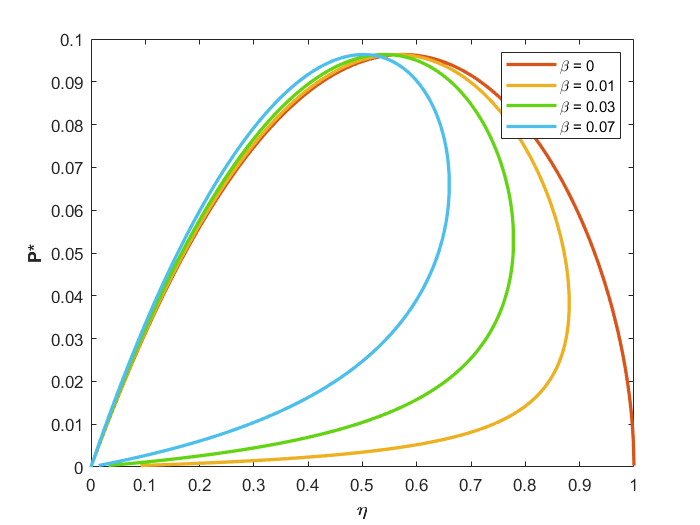
\includegraphics[width=0.6\textwidth]{Images/Ordinary Carnot P vs Eta.png}
    \caption{\textit{power output} tak berdimensi \(P^*\) terhadap efisiensi \(\eta\) pada siklus Carnot kuantum dengan variasi pada nilai \(\beta\).}
    \label{fig:OrdinaryCarnotPvsEta}
\end{figure}
\noindent Grafik ini memperjelas poin dari kedua grafik sebelumnya di mana pada keadaan tanpa disipasi, pada \(r\rightarrow+\infty\), akan didapat efisiensi sempurna namun tanpa adanya \textit{power output}. Hal ini dapat terjadi lantaran waktu yang dibutuhkan untuk menyelesaikan 1 siklus menjadi tak hingga lamanya. Atau dapat ditulis \(\tau\rightarrow+\infty\). Namun pada keadaan dengan disipasi, grafik terlihat seperti \textit{loop} di mana efisiensi menjadi tak bisa mendapat nilai sempurna dan berbalik ke arah 0 setelah titik tertentu. \cite{Wang2012Optimization}

\subsection{Siklus Otto Kuantum}
Siklus yang relevan berikutnya adalah siklus Otto. Siklus ini mengalami keluar masuk panas melalui proses isovolumetris ditengahi oleh ekspansi dan kompresi isoentropis, Gambaran proses dari siklus Otto dapat diilustrasikan sebagai berikut:
\begin{figure} [H]
    \centering
    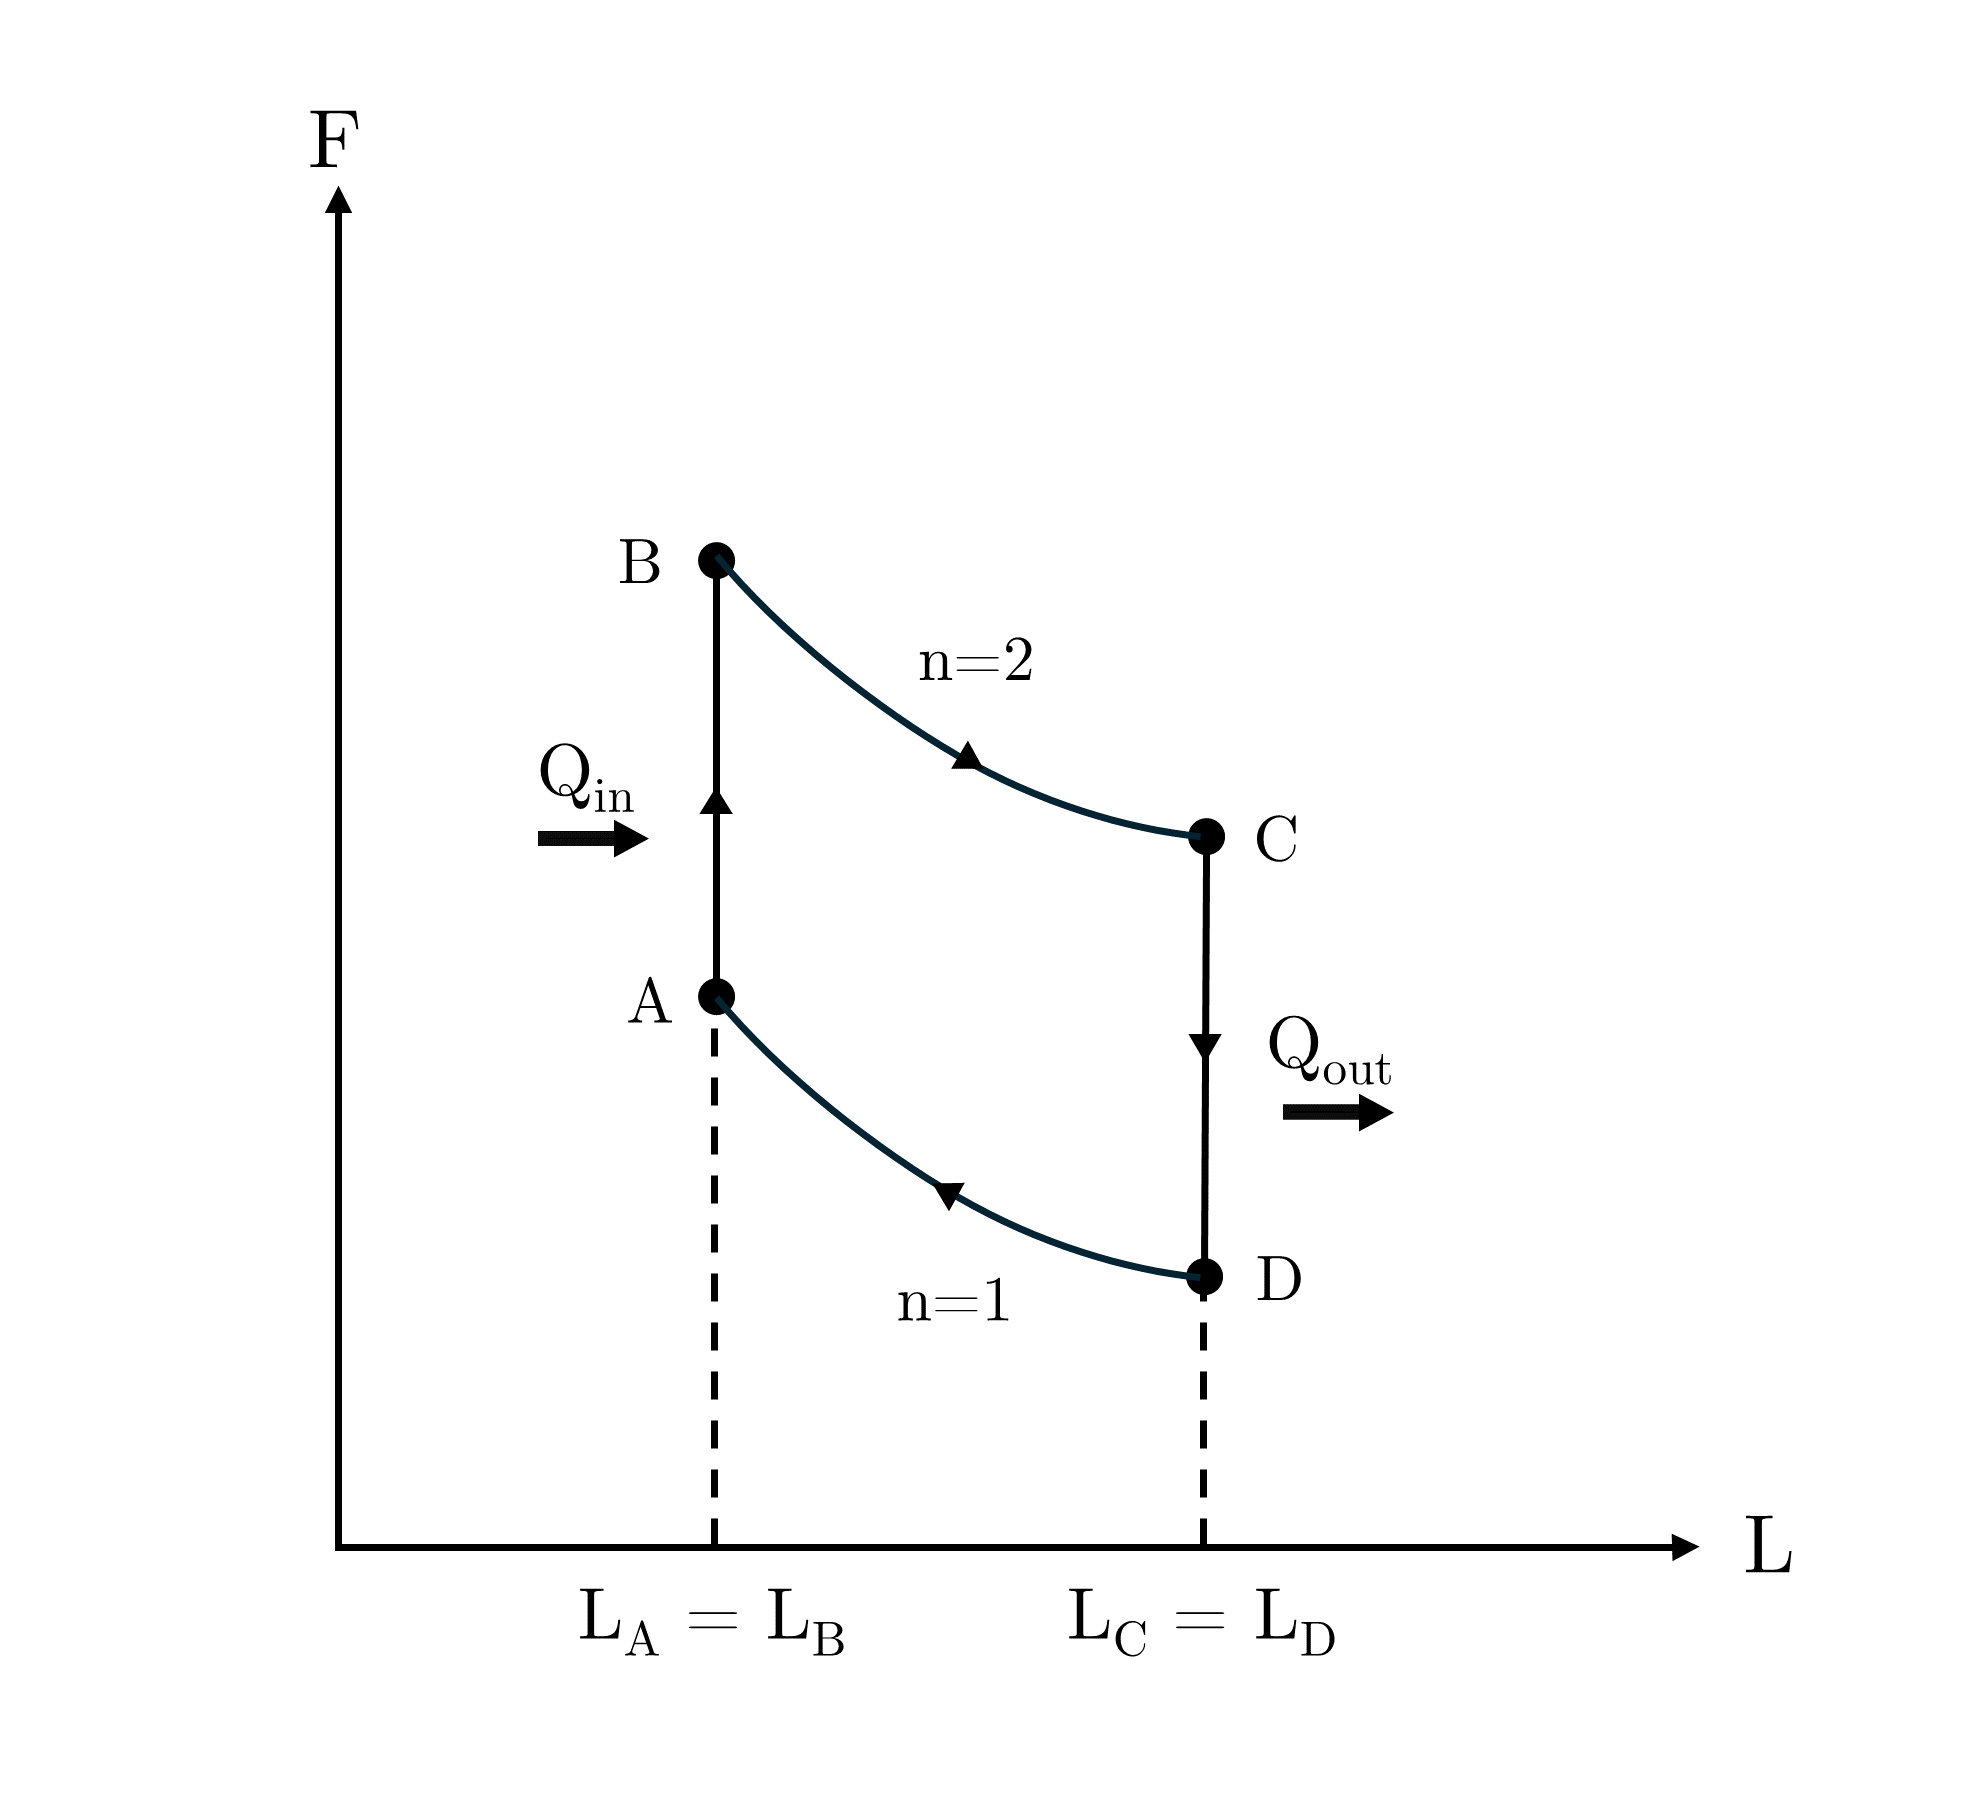
\includegraphics[width=0.5\textwidth]{Images/Quantum Otto Cycle.png}
    \caption{Siklus Otto pada bidang F,L. Siklus ini terdiri dari 4 segmen yang reversibel. \(AB\) adalah pembakaran isovolume, \(BC\) adalah ekspansi adiabatis, \(CD\) adalah pembuangan isovolume, dan \(DA\) adalah kompresi adiabatis. \protect\cite{Thomas2011Coupled}}
    \label{fig:QOttoCycle}
\end{figure}
\par Siklus ini dimulai dengan segmen \(AB\) di mana panas masuk melalui proses isovolume. Tembok kanan tidak bergerak, karenanya pada gambar \ref{fig:QOttoCycle} dituliskan \(L_A = L_B\). Namun tingkatan energi eigen dan rata-rata energi partikel tetap meningkat dikarenakan ada panas yang masuk. Pada siklus ini, panas yang masuk ke sistem dapat dihitung secara langsung sebagai berikut:
\begin{align}
    Q_{AB} = \Delta U_{AB} + \dot{Q_r}\tau
\end{align}
Di sini tidak ada kerja yang dilakukan. Karenanya pada persaman hanya terdapat perubahan energi dalam \(\Delta U\) dan disipasi panas \(\dot{Q_r}\tau\). Bentuk rerata energi yang digunakan mirip seperti pada siklus Carnot. Sehingga didapat,
\begin{align}
    Q_{AB} = E_2(L_B) - E_1(L_A) + \dot{Q_r}\tau = \frac{3\hbar^2\pi^2}{2mL_A^2} + \dot{Q_r}\tau \label{eq:RegOttoQab}
    % &= \frac{\hbar^2\pi^2}{2mL_B^2}\cdot 4 - \frac{\hbar^2\pi^2}{2mL_A^2} + \dot{Q_r}\tau \\
    % Q_{AB} &= \frac{3\hbar^2\pi^2}{2mL_A^2} + \dot{Q_r}\tau
\end{align}
Setelah itu proses dilanjutkan dengan ekspansi isoentropis pada segmen \(BC\). Tembok bergerak dari \(L_B\) menuju \(L_C\) tanpa disertai masuk dan keluarnya panas. Dilanjutkan dengan pembuangan panas melalui proses isovolume pada segmen \(CD\). Pada proses ini, tembok kanan kembali tidak bergerak. Namun, tingkatan energi eigen dan rata-rata energi partikel turun dari sebelumnya. Panas yang dikeluarkan dari sistem bisa didapat sebagai berikut:
\begin{align}
    Q_{CD} = |\Delta U_{CD}| + \dot{Q_r}\tau = \frac{3\hbar^2\pi^2}{2mL_C^2} + \dot{Q_r}\tau \label{eq:RegOttoQcd}
    % &= \frac{\hbar^2\pi^2}{2mL_C^2}\cdot 4 - \frac{\hbar^2\pi^2}{2mL_D^2} + \dot{Q_r}\tau \\
    % Q_{AB} &= \frac{3\hbar^2\pi^2}{2mL_C^2} + \dot{Q_r}\tau
\end{align}
Seperti pada siklus sebelumnya, diambil \(L_A\) dan \(L_C\) untuk perhitungan \textit{power output} serta efisiensi. Terakhir, siklus ditutup dengan kompresi isoentropis pada segmen \(DA\) di mana tembok kanan kembali ke posisi awal untuk memulai kembali rangkaian proses dalam siklus.
\par Untuk mendapatkan \textit{power output} dan efisiensi, diperlukan kerja yang dilakukan oleh sistem. Pada siklus ini kerja \(W\) dihitung menggunakan persamaan (\ref{eq:RegOttoQab}) dan (\ref{eq:RegOttoQcd}) sebagai berikut:
\begin{align}
    W &= Q_{AB} - Q_{CD} = \frac{3\hbar^2\pi^2}{2mL_C^2}(r^2 - 1)
    % &= \frac{3\hbar^2\pi^2}{2m}\left(\frac{1}{L_A^2} - \frac{1}{L_C^2}\right) \\
\end{align}
Di sini, digunakan parameter ekspansi \(L_C = rL_A\) yang sama seperti siklus sebelumnya. Dengan begitu, \textit{power output} dapat dihitung. Definisi dari waktu total satu siklus pada siklus ini sama seperti pada persamaan \ref{eq:TauDef}.
\begin{align}
    P = \frac{W}{\tau} = \frac{3\hbar^2\pi^2\overline{\nu}}{4mL_A^3}\left(\frac{r^2 - 1}{r^3 - r^2}\right) 
    % &= \frac{3\hbar^2\pi^2}{2mL_C^2}(r^2 - 1)\cdot \frac{\overline{\nu}}{2(L_C-L_A)} \\
\end{align}
Dengan begitu, \textit{power output} tak berdimensinya adalah
\begin{align}
    P^* = \frac{3}{4}\left(\frac{r^2 - 1}{r^3 - r^2}\right)
\end{align}
Dengan \(A = \hbar^2\pi^2\overline{\nu}/mL_A^3\). Selanjutnya efisiensi dari siklus ini dapat dihitung sebagai berikut:
\begin{align}
    \eta = \frac{W}{Q_{AB}} = \frac{\frac{3\hbar^2\pi^2}{2mL_C^2}(r^2 - 1)}{\frac{3\hbar^2\pi^2}{2mL_A^2} + \frac{2\dot{Q_r}(L_C - L_A)}{\overline{\nu}}}
\end{align}
Karena yang ditinjau adalah \textit{power output} tak berdimensi, maka efisiensi perlu dibuat tak berdimensi juga. Untuk itu, diasumsikan disipasi panas memiliki bentuk
\begin{align}
    \dot{Q_r} = \beta\frac{3\hbar^2\pi^2\overline{\nu}}{4mL_A^3}
\end{align}
Sehingga didapatkan bentuk efisiensi sebagai berikut:
\begin{align}
    % \eta &= \frac{\frac{3\hbar^2\pi^2}{2mL_C^2}(r^2 - 1)}{\frac{3\hbar^2\pi^2}{2mL_A^2} + \frac{2(L_C - L_A)}{\overline{\nu}} \cdot \beta\frac{3\hbar^2\pi^2\overline{\nu}}{4mL_A^3}} \\
    % &= \frac{r^2 - 1}{r^2(1 + \beta(r - 1))} \\
    \eta = \frac{1 - \left(\frac{1}{r}\right)^2}{1 + \beta(r - 1)}
\end{align}
\par Dari persamaan yang telah didapatkan, dapat dibuat 3 grafik untuk memperjelas perilaku siklus Otto kuantum yang ditinjau. Pertama adalah grafik daya tak berdimensi \(P^*\) terhadap \(r\).
\begin{figure} [H]
    \centering
    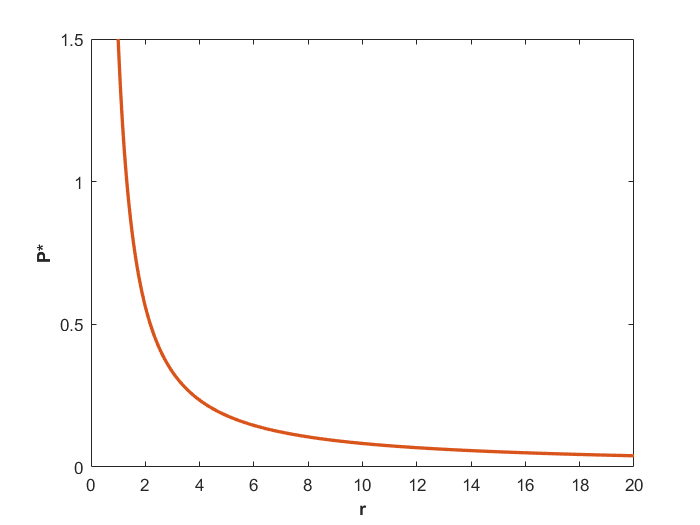
\includegraphics[width=0.6\textwidth]{Images/Ordinary Otto P vs r.png}
    \caption{\textit{power output} tak berdimensi \(P^*\) terhadap \(r\) pada siklus Otto kuantum.}
    \label{fig:OrdinaryOttoPvsR}
\end{figure}
\noindent Dapat dilihat bahwa tidak seperti siklus Carnot, \textit{power output} siklus Otto tidak dimulai dari 0 pada \(r=1\) yang mana batas di mana efisiensinya 0. Melainkan, nilai \textit{power output} tak berdimensinya dimulai dari 1.5 dan terus menurun seiring kenaikan \(r\) dan akan konvergensi ke \(P^*=0\). Grafik berikutnya adalah efisiensi \(\eta\) terhadap \(r\).
\begin{figure} [H]
    \centering
    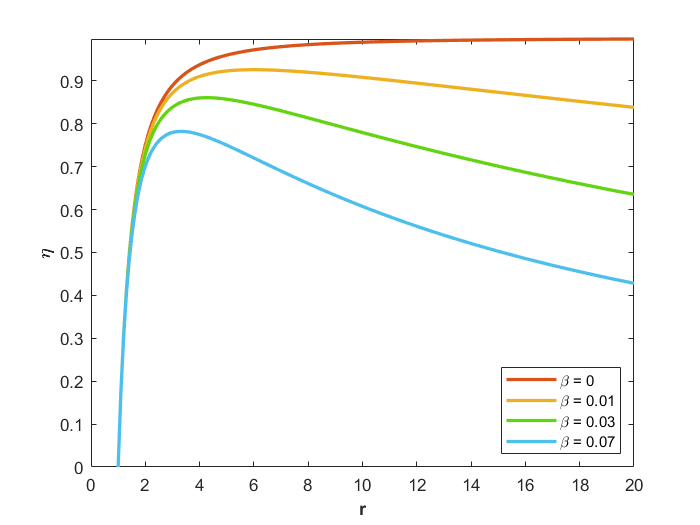
\includegraphics[width=0.6\textwidth]{Images/Ordinary Otto Eta vs r.png}
    \caption{Efisiensi \(\eta\) terhadap \(r\) pada siklus Otto kuantum dengan variasi terhadap parameter disipasi \(\beta\).}
    \label{fig:OrdinaryOttoEtavsR}
\end{figure}
\noindent Grafik \(\eta\) terhadap \(r\) yang didapatkan tidak jauh berbeda polanya dengan siklus Carnot. Hanya saja, nilai efisiensi real positifnya dimulai dari \(r=1\) tidak seperti siklus Carnot yang dimulai dari \(r=2\). Grafik terakhir untuk siklus ini adalah \(P^*\) terhadap \(\eta\) yang berfungsi untuk memperjelas poin yang sudah disampaikan pada 2 grafik sebelumnya.
\begin{figure} [H]
    \centering
    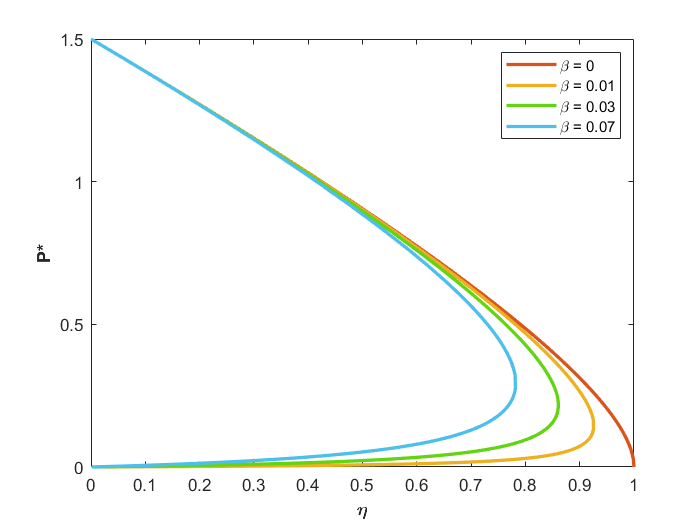
\includegraphics[width=0.6\textwidth]{Images/Ordinary Otto P vs Eta.png}
    \caption{\textit{power output} tak berdimensi \(P^*\) terhadap efisiensi \(\eta\) pada siklus Otto kuantum dengan variasi terhadap parameter disipasi \(\beta\).}
    \label{fig:OrdinaryOttoPvsEta}
\end{figure}
\noindent Pada grafik tersebut, ditunjukkan bahwa saat \(\eta \rightarrow 0\) karena \(r \rightarrow 1\), \textit{power output} dari semua variasi akan konvergensi ke 1.5. Hanya saja, seiring naiknya nilai \(r\), pada keadaan tanpa disipasi \(\beta = 0\), akan didapati efisiensi mendekati 100\% dengan \textit{power output} mendekati 0. Sedangkan pada keadaan dengan disipasi, tidak dimungkinkan efisiensi mencapai 100\% karena terdapat titik balik di mana kenaikan \(r\) akan berakibat penurunan efisiensi. Hal ini secara sekilas tidak intuitif karena efisiensi rendah tapi menghasilkan daya tinggi. Namun hal ini dimungkinkan untuk siklus ini karena saat pertukaran panas, tidak ada kerja yang dilakukan. Semua kerja dilakukan saat proses isoentropis. Sehingga waktu yang dibutuhkan untuk menyelesaikan 1 siklus dapat dibuat sangat kecil. Hal ini mengakibatkan kecilnya kerja yang dilakukan dikompensasi oleh banyaknya siklus yang terjadi. Yang mana membuat \textit{power output} tidak 0 saat \(r \rightarrow 0\). \cite{Pena2020QHE}

\subsection{Siklus Brayton Kuantum}
\par Lalu siklus terakhir yang relevan dengan tulisan ini adalah siklus Brayton yang terdiri dari panas keluar masuk melalui proses isobarik yang ditengahi oleh kompresi dan ekspansi adiabatis. Karena pada tinjauan 1 dimensi luas kehilangan makna, maka proses isobarik bukan ditinjau tekanan konstan seperti proses klasik. Melainkan gaya yang konstan karena definisi tekanan adalah gaya per satuan luas. Gambaran proses dari siklus Brayton dapat diilustrasikan sebagai berikut:
\begin{figure} [H]
    \centering
    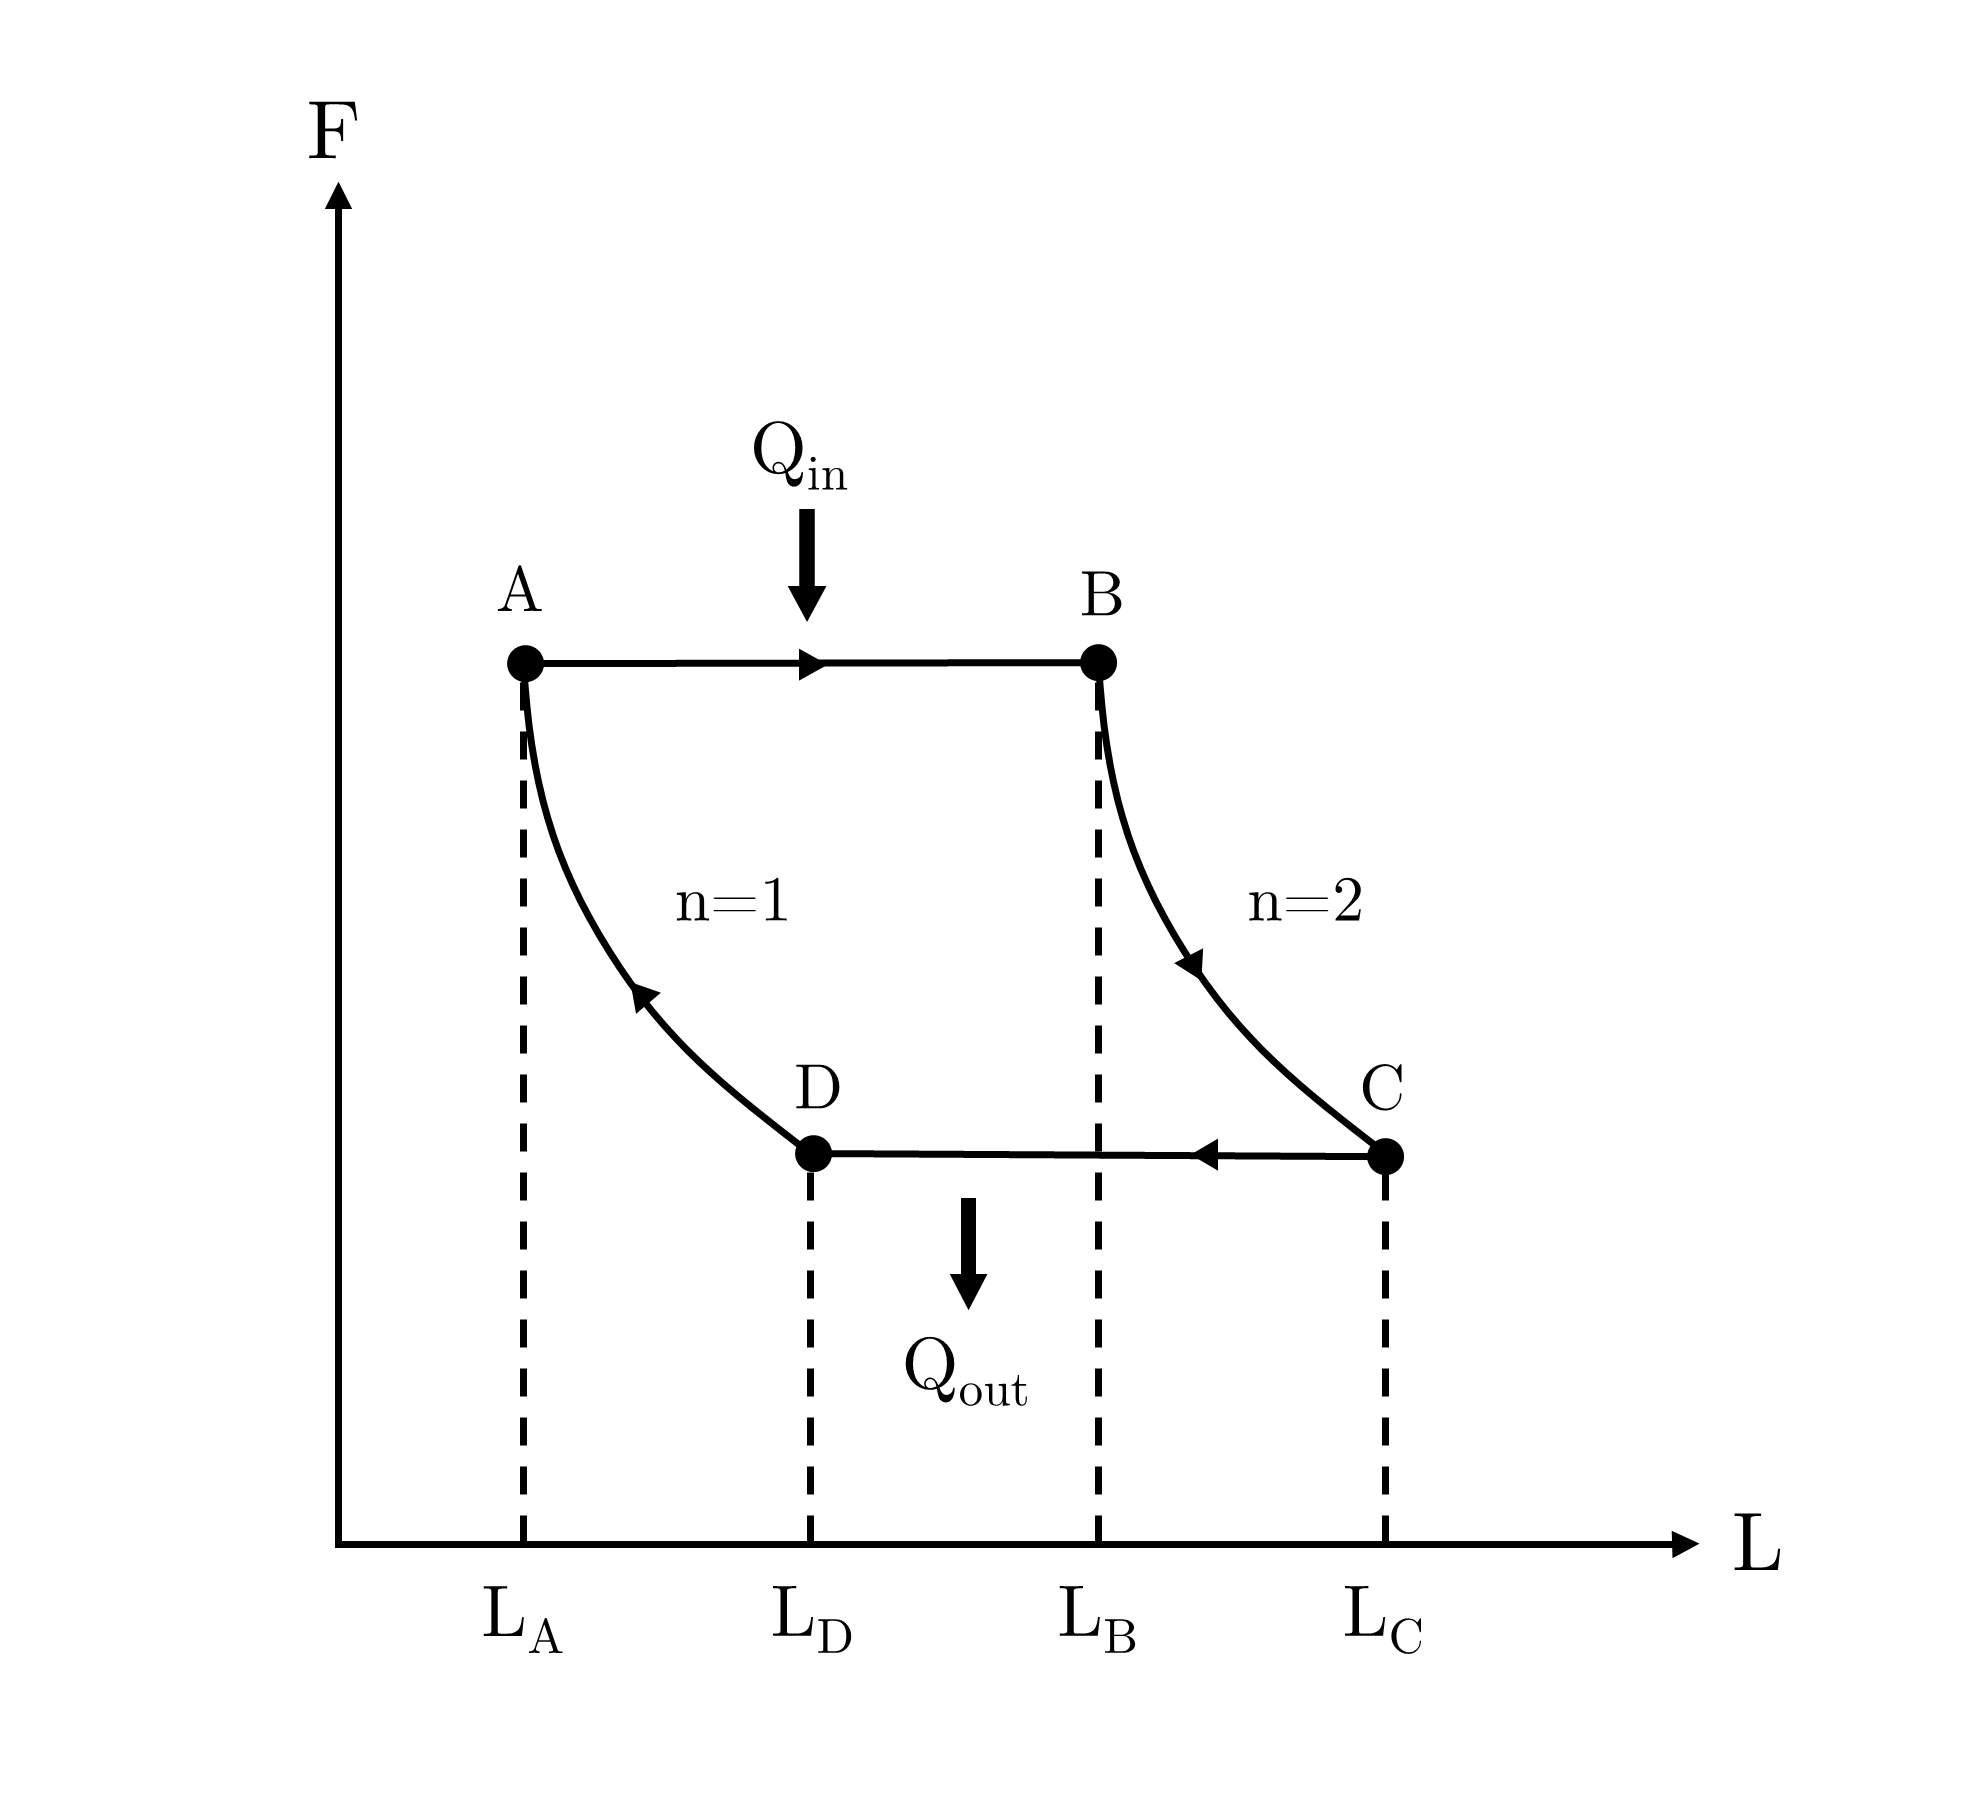
\includegraphics[width=0.5\textwidth]{Images/Quantum Brayton Cycle.png}
    \caption{Siklus Brayton pada bidang F,L. Siklus ini terdiri dari 4 segmen reversibel. \(AB\) adalah ekspansi isobarik, \(BC\) adalah ekspansi adiabatis, \(CD\) adalah kompresi isobarik, dan \(DA\) adalah kompresi adiabatis. \protect\cite{Huang2013Brayton}}
    \label{fig:QBraytonCycle}
\end{figure}
\par Siklus ini dimulai pada segmen \(AB\) di mana panas masuk melalui proses isobarik. Tembok kanan bergerak dari \(L_A\) menuju \(L_B\). Tingkatan energi eigen serta rerata energi partikel naik, namun tanpa disertai dengan perubahan gaya. Secara matematis dapat ditulis sebagai \(F_{AB}(L) = F(L_A) = F(L_B)\). Hubungan gaya konstan ini memberi hubungan lebar sumur \(L_B = 4^\frac{1}{3}L_A\) yang selanjutnya digunakan untuk mendapatkan kerja yang dilakukan selama proses masuknya panas.
% \begin{align}
%     \frac{\hbar^2\pi^2}{mL_A^3} &= \frac{\hbar^2\pi^2}{mL_B^3}\cdot 4 \\
%     L_B^3 &= 4L_A^3 \\
%     L_B &= 4^\frac{1}{3}L_A
% \end{align}
\begin{align}
    W_{AB} &= \int_{L_A}^{L_B} F_{AB} \hspace{1px} dL = \frac{\hbar^2\pi^2}{mL_A^2}(4^\frac{1}{3} - 1) \label{eq:RegBraytonWab}
    % &= \frac{\hbar^2\pi^2}{mL_A^3} \int_{L_A}^{L_B} dL \\
    % &= \frac{\hbar^2\pi^2}{mL_A^3} (L_B - L_A) \\
    % &= \frac{\hbar^2\pi^2}{mL_A^3} (4^\frac{1}{3}L_A - L_A)  \\
\end{align}
Selain itu, dari hubungan lebar sumur tersebut juga dapat ditentukan perubahan energi dalamnya.
\begin{align}
    \Delta U_{AB} = E_2(L_B) - E_1(L_A) = \frac{\hbar^2\pi^2}{2mL_A^2}(4^\frac{1}{3} - 1) \label{eq:RegBraytonUab}
    % &= \frac{\hbar^2\pi^2}{2mL_B^2}\cdot 4 - \frac{\hbar^2\pi^2}{2mL_A^2} \\
    % &= \frac{\hbar^2\pi^2}{2m}\left(\frac{4}{(4^\frac{1}{3}L_A)^2} - \frac{1}{L_A^2} \right)\\
\end{align}
Kerja dan perubahan energi dalam pada persamaan (\ref{eq:RegBraytonWab}) dan (\ref{eq:RegBraytonUab}) ini kemudian digunakan untuk mendapatkan besaran panas yang masuk ke dalam sistem. 
\begin{align}
    Q_{AB} = W_{AB} + \Delta U_{AB} + \dot{Q_r}\tau = \frac{3\hbar^2\pi^2}{2mL_A^2}(4^\frac{1}{3} - 1) + \dot{Q_r}\tau \label{eq:RegBraytonQab}
    % &= \frac{\hbar^2\pi^2}{mL_A^2}(4^\frac{1}{3} - 1) + \frac{\hbar^2\pi^2}{2mL_A^2}(4^\frac{1}{3} - 1) + \dot{Q_r}\tau \\
\end{align}
Setelah itu, proses berlanjut dengan ekspansi isoentropis di mana tidak ada panas yang masuk ataupun keluar dan entropi berada pada keadaan konstan. Tembok kanan juga bergerak dari \(L_B\) menuju \(L_C\). Tingkatan energi eigen pada proses ini tidak berubah namun rerata energi partikel tetap berubah.
\par Siklus dilanjutkan dengan pembuangan panas melalui proses isobarik pada segmen \(CD\). Pada segmen ini, tembok bergerak dari \(L_C\) menuju \(L_D\) dan tingkatan energi eigen turun ke keadaan dasar dikarenakan keluarnya panas. Karena proses ini isobarik, maka gaya yang bekerja pada tembok haruslah konstan. Keadaan ini dapat ditulis sebagai \(F_{CD}(L) = F(L_C) = F(L_D)\). Gaya yang konstan ini memberi hubungan lebar sumur \(L_D = 4^{-\frac{1}{3}} L_C\). Dengan begitu, besaran kerja yang dilakukan selama pembuangan panas dapat dihitung.
\begin{align}
    W_{CD} =  \int_{L_C}^{L_D} F_{CD}(L) dL = - \frac{\hbar^2\pi^2}{mL_C^3}\cdot 4^\frac{2}{3} (4^\frac{1}{3} - 1) \label{eq:RegBraytonWcd}
    % &= \frac{\hbar^2\pi^2}{mL_C^3}\cdot 4 \int_{L_C}^{L_D} dL \\
    % &= - \frac{\hbar^2\pi^2}{mL_C^3}\cdot 4(L_C - L_D) \\
    % &= - \frac{\hbar^2\pi^2}{mL_C^3}\cdot 4(L_C - 4^{-\frac{1}{3}}L_C) \\
\end{align}
Selain itu, hubungan  \(L_C\) dan \(L_D\) juga dapat digunakan untuk mencari besaran perubahan energi dalam yang terjadi.
\begin{align}
    \Delta U_{CD} = E_2(L_B) - E_1(L_A) = -\frac{\hbar^2\pi^2}{2mL_C^2}\cdot 4^\frac{2}{3}(4^\frac{1}{3}-1) \label{eq:RegBraytonUcd}
    % &= \frac{\hbar^2\pi^2}{2mL_C^2}\cdot 4 - \frac{\hbar^2\pi^2}{2mL_D^2} \\
    % &= \frac{\hbar^2\pi^2}{2m}\left(\frac{4}{L_C^2} - \frac{1}{4^{(-\frac{1}{3}L_C)^2}}\right) \\
    % &= \frac{\hbar^2\pi^2}{2mL_C^2}(4-4^\frac{2}{3}) \\
    % &= \frac{\hbar^2\pi^2}{2mL_C^2}\cdot 4(1-4^{-\frac{1}{3}}) \\
\end{align}
Dengan begitu, panas yang keluar dari sistem bisa didapatkan menggunakan persamaan (\ref{eq:RegBraytonWcd}) dan (\ref{eq:RegBraytonUcd}) sebagai berikut:
\begin{align}
    Q_{CD} = |W_{CD}| + |\Delta U_{CD}| + \dot{Q_r}\tau = \frac{3\hbar^2\pi^2}{2mL_C^2}\cdot 4^\frac{2}{3}(4^\frac{1}{3}-1) + \dot{Q_r}\tau \label{eq:RegBraytonQcd}
    % &= \frac{\hbar^2\pi^2}{mL_C^3}\cdot 4^\frac{2}{3} (4^\frac{1}{3} - 1) + \frac{\hbar^2\pi^2}{2mL_C^2}\cdot 4^\frac{2}{3}(4^\frac{1}{3}-1) + \dot{Q_r}\tau \\
\end{align}
Terakhir adalah proses kompresi isoentropis pada segmen \(DA\) di mana posisi tembok kembali ke keadaan semula untuk memulai kembali siklus dari awal. 
\par Dari besaran panas yang masuk dan keluar dari sistem pada persamaan (\ref{eq:RegBraytonQab}) dan (\ref{eq:RegBraytonQcd}), besaran kerja yang dilakukan selama 1 siklus dapat diketahui. Pada siklus ini, dianggap \(W_{BC}-W_{DA}=0\) \cite{MIT_BraytonCycle}. 
\begin{align}
    W = Q_{AB} - Q_{CD} = \frac{3\hbar^2\pi^2}{2mL_C^2}(4^\frac{1}{3} - 1)(r^2 - 4^\frac{2}{3})
    % &= \frac{3\hbar^2\pi^2}{2mL_A^2}(4^\frac{1}{3} - 1) - \frac{3\hbar^2\pi^2}{2mL_C^2}\cdot 4^\frac{2}{3}(4^\frac{1}{3}-1) \\
    % &=  \frac{3\hbar^2\pi^2}{2m}(4^\frac{1}{3} - 1) \left(\frac{1}{L_A^2} - \frac{4^\frac{2}{3}}{L_C^2} \right) \\
\end{align}
Besaran kerja tersebut kemudian digunakan untuk mendapatkan \textit{power output} serta efisieni. \textit{power output} dapat diketahui dengan cara:
\begin{align}
    P = \frac{W}{\tau} =\frac{3\hbar^2\pi^2\overline{\nu}}{4mL_A^3}(4^\frac{1}{3} - 1)\frac{r^2 - 4^\frac{2}{3}}{r^3 - r^2}
    % &= \frac{3\hbar^2\pi^2}{2mL_C^2}(4^\frac{1}{3} - 1)(r^2 - 4^\frac{2}{3}) \frac{\overline{\nu}}{2(L_C - L_A)} \\
\end{align}
Dengan begitu, \textit{power output} tak berdimensinya adalah
\begin{align}
    P^* = \frac{3}{4}(4^\frac{1}{3} - 1)\frac{r^2 - 4^\frac{2}{3}}{r^3 - r^2}
\end{align}
Dengan \(A = \hbar^2\pi^2\overline{\nu}/mL_A^3\). Selanjutnya adalah efisiensi yang dapat dihitung sebagai berikut:
\begin{align}
    \eta = \frac{W}{Q_{AB}} = \frac{\frac{3\hbar^2\pi^2}{2mL_C^2}(4^\frac{1}{3} - 1)(r^2 - 4^\frac{2}{3})}{\frac{3\hbar^2\pi^2}{2mL_A^2}(4^\frac{1}{3} - 1) + \frac{2\dot{Q_r}(L_C - L_A)}{\overline{\nu}}}
\end{align}
Untuk menghilangkan dimensi dari efisiensi, diasumsikan bentuk \(\dot{Q_r}\) dari siklus ini adalah,
\begin{align}
    \dot{Q_r} = \beta\frac{3\hbar^2\pi^2}{4mL_A^3}(4^\frac{1}{3} - 1)
\end{align}
Sehingga didapatkan bentuk efisiensi sebagai berikut:
\begin{align}
    % \eta &= \frac{\frac{3\hbar^2\pi^2}{2mL_C^2}(4^\frac{1}{3} - 1)(r^2 - 4^\frac{2}{3})}{\frac{3\hbar^2\pi^2}{2mL_A^2}(4^\frac{1}{3} - 1) + \frac{2(L_C - L_A)}{\overline{\nu}} \cdot \beta\frac{3\hbar^2\pi^2}{4mL_A^3}(4^\frac{1}{3} - 1)} \\
    \eta &= \frac{1 - \left(\frac{4^\frac{1}{3}}{r}\right)^2}{1 + \beta(r-1)}
\end{align}
\par Seperti 2 siklus sebelumnya, pada siklus ini dapat dibuat 3 grafik yang menunjukkan perilaku parameter \(r\) dan \(\beta\) terhadap \textit{power output} serta efisiensi siklus. Pertama adalah grafik \textit{power output} tak berdimensi \(P^*\) terhadap \(r\).
\begin{figure} [H]
    \centering
    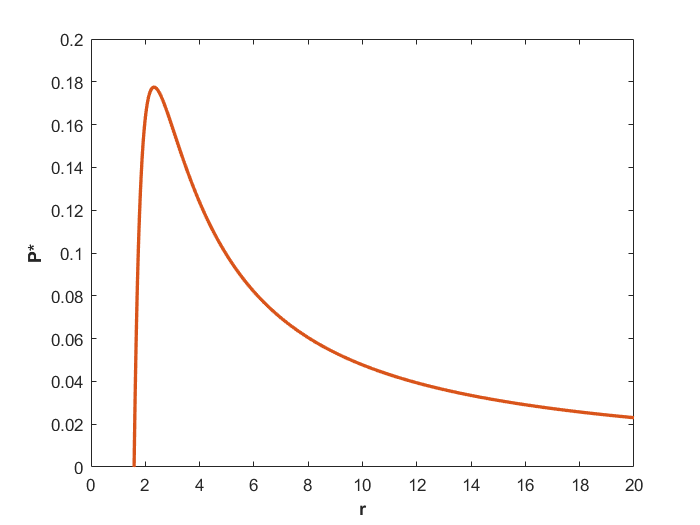
\includegraphics[width=0.6\textwidth]{Images/Ordinary Brayton P vs r.png}
    \caption{\textit{power output} tak berdimensi \(P^*\) terhadap \(r\) pada siklus Brayton kuantum.}
    \label{fig:OrdinaryBraytonPvsR}
\end{figure}
\noindent Bentuk grafiknya secara umum mirip seperti siklus Carnot. Hanya saja nilai \textit{power output} yang real positif dimulai dari \(r \approx 1.59\). Dari titik itu, kenaikan \(r\) mengakibatkan kenaikan daya secara cepat hingga sampai ke titik balik. Setelahnya, kenaikan \(r\) akan menyebabkan penurunan daya hingga konvergensi di \(P^*=0\). Grafik berikutnya adalah efisiensi \(\eta\) terhadap \(r\).
\begin{figure} [H]
    \centering
    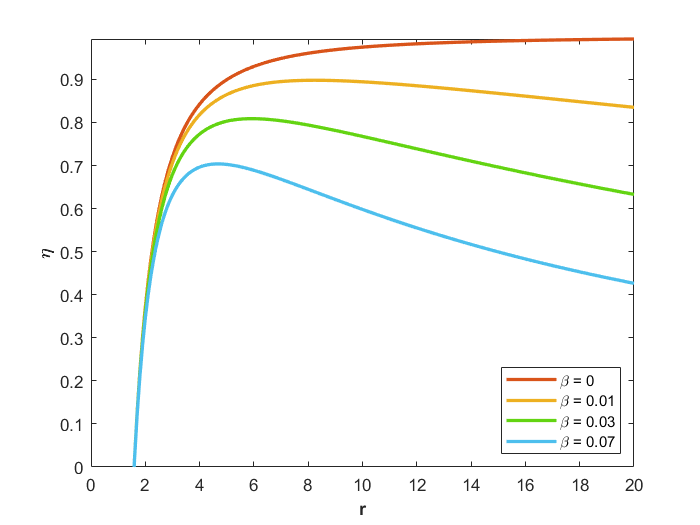
\includegraphics[width=0.6\textwidth]{Images/Ordinary Brayton Eta vs r.png}
    \caption{Efisiensi \(\eta\) terhadap \(r\) pada siklus Brayton kuantum dengan variasi terhadap parameter disipasi \(\beta\).}
    \label{fig:OrdinaryBraytonEtavsR}
\end{figure}
\noindent Pada keadaan tanpa disipasi (\(\beta=0\)), efisiensi akan konvergensi di \(\eta=1\) seiring kenaikan \(r\). Sedangkan pada keadaan dengan disipasi, akan terddapat titik balik yang setelahnya kenaikan \(r\) akan menurunkan \(\eta\) dan akan konvergensi di \(\eta=0\). Sama seperti daya, nilai efisiensi real positif juga dimulai dari \(r \approx 1.59\).
\begin{figure} [H]
    \centering
    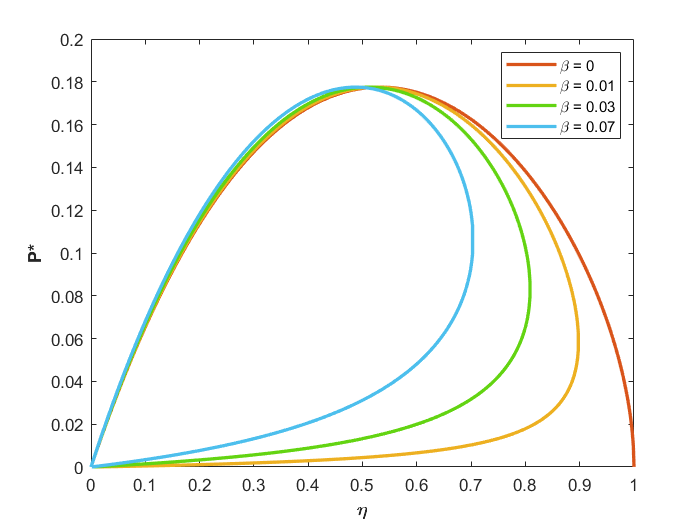
\includegraphics[width=0.6\textwidth]{Images/Ordinary Brayton P vs Eta.png}
    \caption{\textit{power output} tak berdimensi \(P^*\) terhadap efisiensi \(\eta\) pada siklus Brayton kuantum dengan variasi terhadap parameter disipasi \(\beta\).}
    \label{fig:OrdinaryBraytonPvsEta}
\end{figure}
\noindent Secara umum, pola grafik \(P^*\) terhadap \(\eta\) nya mirip dengan siklus Carnot. Pembedanya ada pada puncak daya yang lebih tinggi dibanding siklus Carnot. Pada keadaan tanpa disipasi (\(\beta = 0\)), dimungkinkan untuk mencapai efisiensi sempurna. Hanya saja tidak ada daya yang dikeluarkan. Jika ditambahkan disipasi sedikit saja, maka efisiensi menjadi mustahil untuk mencapai 100\%. Di mana efisiensi akan mengalami titik balik dan kembali ke 0 pada nilai \(r\) yang sangat tinggi. \cite{Fikri2020QHE}

% \newpage
% \thispagestyle{empty}
% \vspace*{\fill}
%     \begin{center}
% 	Halaman ini sengaja dikosongkan
%     \end{center}
% \vspace*{\fill}
% \pagebreak